\documentclass[twoside]{book}

% Packages required by doxygen
\usepackage{fixltx2e}
\usepackage{calc}
\usepackage{doxygen}
\usepackage[export]{adjustbox} % also loads graphicx
\usepackage{graphicx}
\usepackage[utf8]{inputenc}
\usepackage{makeidx}
\usepackage{multicol}
\usepackage{multirow}
\PassOptionsToPackage{warn}{textcomp}
\usepackage{textcomp}
\usepackage[nointegrals]{wasysym}
\usepackage[table]{xcolor}

% Font selection
\usepackage[T1]{fontenc}
\usepackage[scaled=.90]{helvet}
\usepackage{courier}
\usepackage{amssymb}
\usepackage{sectsty}
\renewcommand{\familydefault}{\sfdefault}
\allsectionsfont{%
  \fontseries{bc}\selectfont%
  \color{darkgray}%
}
\renewcommand{\DoxyLabelFont}{%
  \fontseries{bc}\selectfont%
  \color{darkgray}%
}
\newcommand{\+}{\discretionary{\mbox{\scriptsize$\hookleftarrow$}}{}{}}

% Page & text layout
\usepackage{geometry}
\geometry{%
  a4paper,%
  top=2.5cm,%
  bottom=2.5cm,%
  left=2.5cm,%
  right=2.5cm%
}
\tolerance=750
\hfuzz=15pt
\hbadness=750
\setlength{\emergencystretch}{15pt}
\setlength{\parindent}{0cm}
\setlength{\parskip}{3ex plus 2ex minus 2ex}
\makeatletter
\renewcommand{\paragraph}{%
  \@startsection{paragraph}{4}{0ex}{-1.0ex}{1.0ex}{%
    \normalfont\normalsize\bfseries\SS@parafont%
  }%
}
\renewcommand{\subparagraph}{%
  \@startsection{subparagraph}{5}{0ex}{-1.0ex}{1.0ex}{%
    \normalfont\normalsize\bfseries\SS@subparafont%
  }%
}
\makeatother

% Headers & footers
\usepackage{fancyhdr}
\pagestyle{fancyplain}
\fancyhead[LE]{\fancyplain{}{\bfseries\thepage}}
\fancyhead[CE]{\fancyplain{}{}}
\fancyhead[RE]{\fancyplain{}{\bfseries\leftmark}}
\fancyhead[LO]{\fancyplain{}{\bfseries\rightmark}}
\fancyhead[CO]{\fancyplain{}{}}
\fancyhead[RO]{\fancyplain{}{\bfseries\thepage}}
\fancyfoot[LE]{\fancyplain{}{}}
\fancyfoot[CE]{\fancyplain{}{}}
\fancyfoot[RE]{\fancyplain{}{\bfseries\scriptsize Generated by Doxygen }}
\fancyfoot[LO]{\fancyplain{}{\bfseries\scriptsize Generated by Doxygen }}
\fancyfoot[CO]{\fancyplain{}{}}
\fancyfoot[RO]{\fancyplain{}{}}
\renewcommand{\footrulewidth}{0.4pt}
\renewcommand{\chaptermark}[1]{%
  \markboth{#1}{}%
}
\renewcommand{\sectionmark}[1]{%
  \markright{\thesection\ #1}%
}

% Indices & bibliography
\usepackage{natbib}
\usepackage[titles]{tocloft}
\setcounter{tocdepth}{3}
\setcounter{secnumdepth}{5}
\makeindex

% Hyperlinks (required, but should be loaded last)
\usepackage{ifpdf}
\ifpdf
  \usepackage[pdftex,pagebackref=true]{hyperref}
\else
  \usepackage[ps2pdf,pagebackref=true]{hyperref}
\fi
\hypersetup{%
  colorlinks=true,%
  linkcolor=blue,%
  citecolor=blue,%
  unicode%
}

% Custom commands
\newcommand{\clearemptydoublepage}{%
  \newpage{\pagestyle{empty}\cleardoublepage}%
}

\usepackage{caption}
\captionsetup{labelsep=space,justification=centering,font={bf},singlelinecheck=off,skip=4pt,position=top}

%===== C O N T E N T S =====

\begin{document}

% Titlepage & ToC
\hypersetup{pageanchor=false,
             bookmarksnumbered=true,
             pdfencoding=unicode
            }
\pagenumbering{alph}
\begin{titlepage}
\vspace*{7cm}
\begin{center}%
{\Large Open\+Space\+Toolkit\+Simulation \\[1ex]\large 0.\+4.\+5.\+3 }\\
\vspace*{1cm}
{\large Generated by Doxygen 1.8.13}\\
\end{center}
\end{titlepage}
\clearemptydoublepage
\pagenumbering{roman}
\tableofcontents
\clearemptydoublepage
\pagenumbering{arabic}
\hypersetup{pageanchor=true}

%--- Begin generated contents ---
\chapter{Open Space Toolkit ▸ Simulation}
\label{index}\hypertarget{index}{}Structure\href{https://github.com/open-space-collective/open-space-toolkit-simulation/actions/workflows/build-test.yml}{\texttt{ }} \href{https://codecov.io/gh/open-space-collective/open-space-toolkit-simulation}{\texttt{ }} \href{https://open-space-collective.github.io/open-space-toolkit-simulation}{\texttt{ }} \href{https://badge.fury.io/gh/open-space-collective\%2Fopen-space-toolkit-simulation}{\texttt{ }} \href{https://badge.fury.io/py/open-space-toolkit-simulation}{\texttt{ }} \href{https://opensource.org/licenses/Apache-2.0}{\texttt{ }}

Spacecraft simulation.

{\itshape This library is still in draft state. Do not use!}\hypertarget{index_autotoc_md1}{}\doxysection{Getting Started}\label{index_autotoc_md1}
Want to get started? This is the simplest and quickest way\+:

\href{https://mybinder.org/v2/gh/open-space-collective/open-space-toolkit/main?urlpath=lab/tree/notebooks}{\texttt{ }}

{\itshape Nothing to download or install! This will automatically start a \href{https://jupyterlab.readthedocs.io/en/stable/}{\texttt{ Jupyter\+Lab}} environment in your browser with Open Space Toolkit libraries and example notebooks ready to use.}\hypertarget{index_autotoc_md2}{}\doxysubsection{Alternatives}\label{index_autotoc_md2}
\hypertarget{index_autotoc_md3}{}\doxysubsubsection{Docker Images}\label{index_autotoc_md3}
\href{https://www.docker.com/}{\texttt{ Docker}} must be installed on your system.\hypertarget{index_autotoc_md4}{}\doxyparagraph{i\+Python}\label{index_autotoc_md4}
The following command will start an \href{https://ipython.org/}{\texttt{ i\+Python}} shell within a container where the O\+S\+Tk components are already installed\+:


\begin{DoxyCode}{0}
\DoxyCodeLine{docker run -\/it openspacecollective/open-\/space-\/toolkit-\/simulation-\/development python3.11 -\/m IPython}
\end{DoxyCode}


Once the shell is up and running, playing with it is easy\+:


\begin{DoxyCode}{0}
\DoxyCodeLine{\textcolor{comment}{\# TBC...}}
\end{DoxyCode}


By default, O\+S\+Tk fetches the ephemeris from J\+PL, Earth Orientation Parameters (E\+OP) and leap second count from I\+E\+RS.

As a result, when running O\+S\+Tk for the first time, it may take a minute to fetch all the necessary data.

{\itshape Tip\+: Use tab for auto-\/completion!}\hypertarget{index_autotoc_md5}{}\doxyparagraph{Jupyter\+Lab}\label{index_autotoc_md5}
The following command will start a \href{https://jupyterlab.readthedocs.io/en/stable/}{\texttt{ Jupyter\+Lab}} server within a container where the O\+S\+Tk components are already installed\+:


\begin{DoxyCode}{0}
\DoxyCodeLine{docker run -\/-\/publish=8888:8888 openspacecollective/open-\/space-\/toolkit-\/simulation-\/jupyter}
\end{DoxyCode}


Once the container is running, access \href{http://localhost:8888/lab}{\texttt{ http\+://localhost\+:8888/lab}} and create a Python 3 Notebook.\hypertarget{index_autotoc_md6}{}\doxysection{Installation}\label{index_autotoc_md6}
\hypertarget{index_autotoc_md7}{}\doxysubsection{C++}\label{index_autotoc_md7}
The binary packages are hosted using \href{https://github.com/open-space-collective/open-space-toolkit-simulation/releases}{\texttt{ Git\+Hub Releases}}\+:


\begin{DoxyItemize}
\item Runtime libraries\+: {\ttfamily open-\/space-\/toolkit-\/simulation-\/\+X.\+Y.\+Z-\/1.\+x86\+\_\+64-\/runtime}
\item C++ headers\+: {\ttfamily open-\/space-\/toolkit-\/simulation-\/\+X.\+Y.\+Z-\/1.\+x86\+\_\+64-\/devel}
\item Python bindings\+: {\ttfamily open-\/space-\/toolkit-\/simulation-\/\+X.\+Y.\+Z-\/1.\+x86\+\_\+64-\/python}
\end{DoxyItemize}\hypertarget{index_autotoc_md8}{}\doxysubsubsection{Debian / Ubuntu}\label{index_autotoc_md8}
After downloading the relevant {\ttfamily .deb} binary packages, install\+:


\begin{DoxyCode}{0}
\DoxyCodeLine{apt install open-\/space-\/toolkit-\/simulation-\/*.deb}
\end{DoxyCode}
\hypertarget{index_autotoc_md9}{}\doxysubsection{Python}\label{index_autotoc_md9}
Install from \href{https://pypi.org/project/open-space-toolkit-simulation/}{\texttt{ Py\+PI}}\+:


\begin{DoxyCode}{0}
\DoxyCodeLine{pip install open-\/space-\/toolkit-\/simulation}
\end{DoxyCode}
\hypertarget{index_autotoc_md10}{}\doxysection{Documentation}\label{index_autotoc_md10}
Documentation is available here\+:


\begin{DoxyItemize}
\item \href{https://open-space-collective.github.io/open-space-toolkit-simulation}{\texttt{ C++}}
\item \href{./bindings/python/docs}{\texttt{ Python}}
\end{DoxyItemize}

$<$details$>$

The library exhibits the following detailed and descriptive structure\+:


\begin{DoxyCode}{0}
\DoxyCodeLine{└── Satellite}
\end{DoxyCode}


$<$/details$>$\hypertarget{index_autotoc_md11}{}\doxysection{Tutorials}\label{index_autotoc_md11}
Tutorials are available here\+:


\begin{DoxyItemize}
\item \href{./tutorials/cpp}{\texttt{ C++}}
\item \href{./tutorials/python}{\texttt{ Python}}
\end{DoxyItemize}\hypertarget{index_autotoc_md12}{}\doxysection{Setup}\label{index_autotoc_md12}
\hypertarget{index_autotoc_md13}{}\doxysubsection{Development Environment}\label{index_autotoc_md13}
Using \href{https://www.docker.com}{\texttt{ Docker}} for development is recommended, to simplify the installation of the necessary build tools and dependencies. Instructions on how to install Docker are available \href{https://docs.docker.com/install/}{\texttt{ here}}.

To start the development environment\+:


\begin{DoxyCode}{0}
\DoxyCodeLine{make start-\/development}
\end{DoxyCode}


This will\+:


\begin{DoxyEnumerate}
\item Build the {\ttfamily openspacecollective/open-\/space-\/toolkit-\/simulation-\/development} Docker image.
\item Create a development environment container with local source files and helper scripts mounted.
\item Start a {\ttfamily bash} shell from the {\ttfamily ./build} working directory.
\end{DoxyEnumerate}

If installing Docker is not an option, you can manually install the development tools (G\+CC, C\+Make) and all required dependencies, by following a procedure similar to the one described in the \href{./docker/development/Dockerfile}{\texttt{ Development Dockerfile}}.\hypertarget{index_autotoc_md14}{}\doxysubsection{Build}\label{index_autotoc_md14}
From the {\ttfamily ./build} directory\+:


\begin{DoxyCode}{0}
\DoxyCodeLine{cmake ..}
\DoxyCodeLine{make}
\end{DoxyCode}


{\itshape Tip\+: {\ttfamily ostk-\/build} simplifies building from within the development environment.}\hypertarget{index_autotoc_md15}{}\doxysubsection{Test}\label{index_autotoc_md15}
To start a container to build and run the tests\+:


\begin{DoxyCode}{0}
\DoxyCodeLine{make test}
\end{DoxyCode}


Or to run them manually\+:


\begin{DoxyCode}{0}
\DoxyCodeLine{./bin/open-\/space-\/toolkit-\/simulation.test}
\end{DoxyCode}


{\itshape Tip\+: {\ttfamily ostk-\/test} simplifies running tests from within the development environment.}\hypertarget{index_autotoc_md16}{}\doxysection{Dependencies}\label{index_autotoc_md16}
\tabulinesep=1mm
\begin{longtabu}spread 0pt [c]{*{4}{|X[-1]}|}
\hline
\PBS\centering \cellcolor{\tableheadbgcolor}\textbf{ Name }&\PBS\centering \cellcolor{\tableheadbgcolor}\textbf{ Version }&\PBS\centering \cellcolor{\tableheadbgcolor}\textbf{ License }&\PBS\centering \cellcolor{\tableheadbgcolor}\textbf{ Link  }\\\cline{1-4}
\endfirsthead
\hline
\endfoot
\hline
\PBS\centering \cellcolor{\tableheadbgcolor}\textbf{ Name }&\PBS\centering \cellcolor{\tableheadbgcolor}\textbf{ Version }&\PBS\centering \cellcolor{\tableheadbgcolor}\textbf{ License }&\PBS\centering \cellcolor{\tableheadbgcolor}\textbf{ Link  }\\\cline{1-4}
\endhead
Pybind11 &2.\+12.\+0 &B\+S\+D-\/3-\/\+Clause &\href{https://github.com/pybind/pybind11}{\texttt{ github.\+com/pybind/pybind11}}  \\\cline{1-4}
Core &main &Apache License 2.\+0 &\href{https://github.com/open-space-collective/open-space-toolkit-core}{\texttt{ github.\+com/open-\/space-\/collective/open-\/space-\/toolkit-\/core}}  \\\cline{1-4}
I/O &main &Apache License 2.\+0 &\href{https://github.com/open-space-collective/open-space-toolkit-io}{\texttt{ github.\+com/open-\/space-\/collective/open-\/space-\/toolkit-\/io}}  \\\cline{1-4}
Mathematics &main &Apache License 2.\+0 &\href{https://github.com/open-space-collective/open-space-toolkit-mathematics}{\texttt{ github.\+com/open-\/space-\/collective/open-\/space-\/toolkit-\/mathematics}}  \\\cline{1-4}
Physics &main &Apache License 2.\+0 &\href{https://github.com/open-space-collective/open-space-toolkit-physics}{\texttt{ github.\+com/open-\/space-\/collective/open-\/space-\/toolkit-\/physics}}  \\\cline{1-4}
Astrodynamics &main &Apache License 2.\+0 &\href{https://github.com/open-space-collective/open-space-toolkit-astrodynamics}{\texttt{ github.\+com/open-\/space-\/collective/open-\/space-\/toolkit-\/astrodynamics}}  \\\cline{1-4}
\end{longtabu}
\hypertarget{index_autotoc_md17}{}\doxysection{Contribution}\label{index_autotoc_md17}
Contributions are more than welcome!

Please read our \mbox{\hyperlink{_c_o_n_t_r_i_b_u_t_i_n_g_8md}{contributing guide}} to learn about our development process, how to propose fixes and improvements, and how to build and test the code.\hypertarget{index_autotoc_md18}{}\doxysection{Special Thanks}\label{index_autotoc_md18}
\href{https://www.loftorbital.com/}{\texttt{ }}\hypertarget{index_autotoc_md19}{}\doxysection{License}\label{index_autotoc_md19}
Apache License 2.\+0 
\chapter{Contributing}
\label{md__c_o_n_t_r_i_b_u_t_i_n_g}
\Hypertarget{md__c_o_n_t_r_i_b_u_t_i_n_g}
{\itshape ⚠ This document is a work in progress.}\hypertarget{md__c_o_n_t_r_i_b_u_t_i_n_g_Introduction}{}\doxysection{Introduction}\label{md__c_o_n_t_r_i_b_u_t_i_n_g_Introduction}
{\itshape To be completed...}\hypertarget{md__c_o_n_t_r_i_b_u_t_i_n_g_Guidelines}{}\doxysection{Guidelines}\label{md__c_o_n_t_r_i_b_u_t_i_n_g_Guidelines}
\hypertarget{md__c_o_n_t_r_i_b_u_t_i_n_g_Codebase}{}\doxysubsection{Codebase}\label{md__c_o_n_t_r_i_b_u_t_i_n_g_Codebase}
\hypertarget{md__c_o_n_t_r_i_b_u_t_i_n_g_C}{}\doxysubsubsection{C++}\label{md__c_o_n_t_r_i_b_u_t_i_n_g_C}
Include order from specific to generic\+:


\begin{DoxyCode}{0}
\DoxyCodeLine{\textcolor{preprocessor}{\#include <OpenSpaceToolkit/Simulation/Orbit.hpp>}}
\DoxyCodeLine{}
\DoxyCodeLine{\textcolor{preprocessor}{\#include <OpenSpaceToolkit/Core/Types/Integer.hpp>}}
\DoxyCodeLine{\textcolor{preprocessor}{\#include <OpenSpaceToolkit/Core/Utilities.hpp>}}
\DoxyCodeLine{}
\DoxyCodeLine{\textcolor{preprocessor}{\#include <map>}}
\DoxyCodeLine{\textcolor{preprocessor}{\#include <string>}}
\end{DoxyCode}


References\+:


\begin{DoxyItemize}
\item \href{https://stackoverflow.com/questions/2762568/c-c-include-file-order-best-practices}{\texttt{ https\+://stackoverflow.\+com/questions/2762568/c-\/c-\/include-\/file-\/order-\/best-\/practices}}
\item \href{https://blog.kowalczyk.info/article/qg/order-of-include-headers-in-cc.html}{\texttt{ https\+://blog.\+kowalczyk.\+info/article/qg/order-\/of-\/include-\/headers-\/in-\/cc.\+html}}
\end{DoxyItemize}\hypertarget{md__c_o_n_t_r_i_b_u_t_i_n_g_Python}{}\doxysubsubsection{Python}\label{md__c_o_n_t_r_i_b_u_t_i_n_g_Python}
{\itshape To be completed...}\hypertarget{md__c_o_n_t_r_i_b_u_t_i_n_g_Version}{}\doxysubsection{Version Control}\label{md__c_o_n_t_r_i_b_u_t_i_n_g_Version}
\hypertarget{md__c_o_n_t_r_i_b_u_t_i_n_g_Rules}{}\doxysubsubsection{Rules}\label{md__c_o_n_t_r_i_b_u_t_i_n_g_Rules}
{\itshape To be completed...}\hypertarget{md__c_o_n_t_r_i_b_u_t_i_n_g_Commit}{}\doxysubsubsection{Commit Messages}\label{md__c_o_n_t_r_i_b_u_t_i_n_g_Commit}
\href{https://chris.beams.io/posts/git-commit/}{\texttt{ How to Write a Git Commit Message}}

Use active form ({\ttfamily Do something}).

Prefix commit messages using the following tags\+:


\begin{DoxyItemize}
\item \mbox{[}feature\mbox{]}
\item \mbox{[}fix\mbox{]}
\item \mbox{[}misc\mbox{]}
\end{DoxyItemize}

Examples\+:


\begin{DoxyCode}{0}
\DoxyCodeLine{[feature] Implement high fidelity orbit propagator}
\end{DoxyCode}



\begin{DoxyCode}{0}
\DoxyCodeLine{[fix] Segmentation fault when fetching ephemeris data}
\end{DoxyCode}
\hypertarget{md__c_o_n_t_r_i_b_u_t_i_n_g_CodeOfConduct}{}\doxysection{Code of Conduct}\label{md__c_o_n_t_r_i_b_u_t_i_n_g_CodeOfConduct}
{\itshape To be completed...} 
\chapter{Tutorial}
\label{md_docs__tutorial}
\Hypertarget{md_docs__tutorial}
Below are examples illustrating a few common use-\/cases.\hypertarget{md_docs__tutorial_Setup}{}\doxysection{Setup}\label{md_docs__tutorial_Setup}
{\itshape To be completed...}\hypertarget{md_docs__tutorial_Examples}{}\doxysection{Examples}\label{md_docs__tutorial_Examples}
{\itshape To be completed...} 
\chapter{Namespace Index}
\doxysection{Namespace List}
Here is a list of all namespaces with brief descriptions\+:\begin{DoxyCompactList}
\item\contentsline{section}{\mbox{\hyperlink{namespaceostk}{ostk}} \\*Apache License 2.\+0 }{\pageref{namespaceostk}}{}
\item\contentsline{section}{\mbox{\hyperlink{namespaceostk_1_1simulation}{ostk\+::simulation}} }{\pageref{namespaceostk_1_1simulation}}{}
\item\contentsline{section}{\mbox{\hyperlink{namespaceostk_1_1simulation_1_1component}{ostk\+::simulation\+::component}} }{\pageref{namespaceostk_1_1simulation_1_1component}}{}
\item\contentsline{section}{\mbox{\hyperlink{namespaceostk_1_1simulation_1_1utilities}{ostk\+::simulation\+::utilities}} }{\pageref{namespaceostk_1_1simulation_1_1utilities}}{}
\end{DoxyCompactList}

\chapter{Hierarchical Index}
\doxysection{Class Hierarchy}
This inheritance list is sorted roughly, but not completely, alphabetically\+:\begin{DoxyCompactList}
\item \contentsline{section}{ostk\+::simulation\+::Component\+Configuration}{\pageref{structostk_1_1simulation_1_1_component_configuration}}{}
\item \contentsline{section}{ostk\+::simulation\+::utility\+::Component\+Holder}{\pageref{classostk_1_1simulation_1_1utility_1_1_component_holder}}{}
\begin{DoxyCompactList}
\item \contentsline{section}{ostk\+::simulation\+::Component}{\pageref{classostk_1_1simulation_1_1_component}}{}
\begin{DoxyCompactList}
\item \contentsline{section}{ostk\+::simulation\+::Satellite}{\pageref{classostk_1_1simulation_1_1_satellite}}{}
\end{DoxyCompactList}
\end{DoxyCompactList}
\item enable\+\_\+shared\+\_\+from\+\_\+this\begin{DoxyCompactList}
\item \contentsline{section}{ostk\+::simulation\+::Component}{\pageref{classostk_1_1simulation_1_1_component}}{}
\end{DoxyCompactList}
\item \contentsline{section}{ostk\+::simulation\+::Entity}{\pageref{classostk_1_1simulation_1_1_entity}}{}
\begin{DoxyCompactList}
\item \contentsline{section}{ostk\+::simulation\+::Component}{\pageref{classostk_1_1simulation_1_1_component}}{}
\end{DoxyCompactList}
\item \contentsline{section}{ostk\+::simulation\+::component\+::Geometry}{\pageref{classostk_1_1simulation_1_1component_1_1_geometry}}{}
\item \contentsline{section}{ostk\+::simulation\+::component\+::Geometry\+Configuration}{\pageref{structostk_1_1simulation_1_1component_1_1_geometry_configuration}}{}
\item \contentsline{section}{ostk\+::simulation\+::Satellite\+Configuration}{\pageref{structostk_1_1simulation_1_1_satellite_configuration}}{}
\item \contentsline{section}{ostk\+::simulation\+::Simulator}{\pageref{classostk_1_1simulation_1_1_simulator}}{}
\item \contentsline{section}{ostk\+::simulation\+::Simulator\+Configuration}{\pageref{structostk_1_1simulation_1_1_simulator_configuration}}{}
\item \contentsline{section}{ostk\+::simulation\+::component\+::State}{\pageref{classostk_1_1simulation_1_1component_1_1_state}}{}
\end{DoxyCompactList}

\chapter{Class Index}
\doxysection{Class List}
Here are the classes, structs, unions and interfaces with brief descriptions\+:\begin{DoxyCompactList}
\item\contentsline{section}{\mbox{\hyperlink{classostk_1_1simulation_1_1_component}{ostk\+::simulation\+::\+Component}} \\*\mbox{\hyperlink{classostk_1_1simulation_1_1_component}{Component}} }{\pageref{classostk_1_1simulation_1_1_component}}{}
\item\contentsline{section}{\mbox{\hyperlink{structostk_1_1simulation_1_1_component_configuration}{ostk\+::simulation\+::\+Component\+Configuration}} }{\pageref{structostk_1_1simulation_1_1_component_configuration}}{}
\item\contentsline{section}{\mbox{\hyperlink{classostk_1_1simulation_1_1utility_1_1_component_holder}{ostk\+::simulation\+::utility\+::\+Component\+Holder}} \\*Generic \mbox{\hyperlink{classostk_1_1simulation_1_1_component}{Component}} holder }{\pageref{classostk_1_1simulation_1_1utility_1_1_component_holder}}{}
\item\contentsline{section}{\mbox{\hyperlink{classostk_1_1simulation_1_1_entity}{ostk\+::simulation\+::\+Entity}} \\*\mbox{\hyperlink{classostk_1_1simulation_1_1_entity}{Entity}} }{\pageref{classostk_1_1simulation_1_1_entity}}{}
\item\contentsline{section}{\mbox{\hyperlink{classostk_1_1simulation_1_1component_1_1_geometry}{ostk\+::simulation\+::component\+::\+Geometry}} \\*\mbox{\hyperlink{classostk_1_1simulation_1_1_component}{Component}} geometry }{\pageref{classostk_1_1simulation_1_1component_1_1_geometry}}{}
\item\contentsline{section}{\mbox{\hyperlink{structostk_1_1simulation_1_1component_1_1_geometry_configuration}{ostk\+::simulation\+::component\+::\+Geometry\+Configuration}} }{\pageref{structostk_1_1simulation_1_1component_1_1_geometry_configuration}}{}
\item\contentsline{section}{\mbox{\hyperlink{classostk_1_1simulation_1_1_satellite}{ostk\+::simulation\+::\+Satellite}} \\*\mbox{\hyperlink{classostk_1_1simulation_1_1_satellite}{Satellite}} }{\pageref{classostk_1_1simulation_1_1_satellite}}{}
\item\contentsline{section}{\mbox{\hyperlink{structostk_1_1simulation_1_1_satellite_configuration}{ostk\+::simulation\+::\+Satellite\+Configuration}} }{\pageref{structostk_1_1simulation_1_1_satellite_configuration}}{}
\item\contentsline{section}{\mbox{\hyperlink{classostk_1_1simulation_1_1_simulator}{ostk\+::simulation\+::\+Simulator}} \\*\mbox{\hyperlink{classostk_1_1simulation_1_1_simulator}{Simulator}} }{\pageref{classostk_1_1simulation_1_1_simulator}}{}
\item\contentsline{section}{\mbox{\hyperlink{structostk_1_1simulation_1_1_simulator_configuration}{ostk\+::simulation\+::\+Simulator\+Configuration}} }{\pageref{structostk_1_1simulation_1_1_simulator_configuration}}{}
\item\contentsline{section}{\mbox{\hyperlink{classostk_1_1simulation_1_1component_1_1_state}{ostk\+::simulation\+::component\+::\+State}} \\*\mbox{\hyperlink{classostk_1_1simulation_1_1_component}{Component}} state }{\pageref{classostk_1_1simulation_1_1component_1_1_state}}{}
\end{DoxyCompactList}

\chapter{File Index}
\doxysection{File List}
Here is a list of all files with brief descriptions\+:\begin{DoxyCompactList}
\item\contentsline{section}{include/\+Open\+Space\+Toolkit/\+Simulation/\mbox{\hyperlink{_component_8hpp}{Component.\+hpp}} }{\pageref{_component_8hpp}}{}
\item\contentsline{section}{include/\+Open\+Space\+Toolkit/\+Simulation/\mbox{\hyperlink{_entity_8hpp}{Entity.\+hpp}} }{\pageref{_entity_8hpp}}{}
\item\contentsline{section}{include/\+Open\+Space\+Toolkit/\+Simulation/\mbox{\hyperlink{_satellite_8hpp}{Satellite.\+hpp}} }{\pageref{_satellite_8hpp}}{}
\item\contentsline{section}{include/\+Open\+Space\+Toolkit/\+Simulation/\mbox{\hyperlink{_simulator_8hpp}{Simulator.\+hpp}} }{\pageref{_simulator_8hpp}}{}
\item\contentsline{section}{include/\+Open\+Space\+Toolkit/\+Simulation/\+Component/\mbox{\hyperlink{_geometry_8hpp}{Geometry.\+hpp}} }{\pageref{_geometry_8hpp}}{}
\item\contentsline{section}{include/\+Open\+Space\+Toolkit/\+Simulation/\+Component/\mbox{\hyperlink{_state_8hpp}{State.\+hpp}} }{\pageref{_state_8hpp}}{}
\item\contentsline{section}{include/\+Open\+Space\+Toolkit/\+Simulation/\+Utility/\mbox{\hyperlink{_component_holder_8hpp}{Component\+Holder.\+hpp}} }{\pageref{_component_holder_8hpp}}{}
\item\contentsline{section}{include/\+Open\+Space\+Toolkit/\+Simulation/\+Utility/\mbox{\hyperlink{_identifier_8hpp}{Identifier.\+hpp}} }{\pageref{_identifier_8hpp}}{}
\item\contentsline{section}{src/\+Open\+Space\+Toolkit/\+Simulation/\mbox{\hyperlink{_component_8cpp}{Component.\+cpp}} }{\pageref{_component_8cpp}}{}
\item\contentsline{section}{src/\+Open\+Space\+Toolkit/\+Simulation/\mbox{\hyperlink{_entity_8cpp}{Entity.\+cpp}} }{\pageref{_entity_8cpp}}{}
\item\contentsline{section}{src/\+Open\+Space\+Toolkit/\+Simulation/\mbox{\hyperlink{_satellite_8cpp}{Satellite.\+cpp}} }{\pageref{_satellite_8cpp}}{}
\item\contentsline{section}{src/\+Open\+Space\+Toolkit/\+Simulation/\mbox{\hyperlink{_simulator_8cpp}{Simulator.\+cpp}} }{\pageref{_simulator_8cpp}}{}
\item\contentsline{section}{src/\+Open\+Space\+Toolkit/\+Simulation/\+Component/\mbox{\hyperlink{_geometry_8cpp}{Geometry.\+cpp}} }{\pageref{_geometry_8cpp}}{}
\item\contentsline{section}{src/\+Open\+Space\+Toolkit/\+Simulation/\+Component/\mbox{\hyperlink{_state_8cpp}{State.\+cpp}} }{\pageref{_state_8cpp}}{}
\item\contentsline{section}{src/\+Open\+Space\+Toolkit/\+Simulation/\+Utility/\mbox{\hyperlink{_component_holder_8cpp}{Component\+Holder.\+cpp}} }{\pageref{_component_holder_8cpp}}{}
\item\contentsline{section}{src/\+Open\+Space\+Toolkit/\+Simulation/\+Utility/\mbox{\hyperlink{_identifier_8cpp}{Identifier.\+cpp}} }{\pageref{_identifier_8cpp}}{}
\end{DoxyCompactList}

\chapter{Namespace Documentation}
\hypertarget{namespaceostk}{}\doxysection{ostk Namespace Reference}
\label{namespaceostk}\index{ostk@{ostk}}


Apache License 2.\+0.  


\doxysubsection*{Namespaces}
\begin{DoxyCompactItemize}
\item 
 \mbox{\hyperlink{namespaceostk_1_1simulation}{simulation}}
\end{DoxyCompactItemize}


\doxysubsection{Detailed Description}
Apache License 2.\+0. 
\hypertarget{namespaceostk_1_1simulation}{}\doxysection{ostk\+::simulation Namespace Reference}
\label{namespaceostk_1_1simulation}\index{ostk::simulation@{ostk::simulation}}
\doxysubsection*{Namespaces}
\begin{DoxyCompactItemize}
\item 
 \mbox{\hyperlink{namespaceostk_1_1simulation_1_1component}{component}}
\item 
 \mbox{\hyperlink{namespaceostk_1_1simulation_1_1utilities}{utilities}}
\end{DoxyCompactItemize}
\doxysubsection*{Classes}
\begin{DoxyCompactItemize}
\item 
class \mbox{\hyperlink{classostk_1_1simulation_1_1_component}{Component}}
\begin{DoxyCompactList}\small\item\em \mbox{\hyperlink{classostk_1_1simulation_1_1_component}{Component}}. \end{DoxyCompactList}\item 
struct \mbox{\hyperlink{structostk_1_1simulation_1_1_component_configuration}{Component\+Configuration}}
\item 
class \mbox{\hyperlink{classostk_1_1simulation_1_1_entity}{Entity}}
\begin{DoxyCompactList}\small\item\em \mbox{\hyperlink{classostk_1_1simulation_1_1_entity}{Entity}}. \end{DoxyCompactList}\item 
class \mbox{\hyperlink{classostk_1_1simulation_1_1_satellite}{Satellite}}
\begin{DoxyCompactList}\small\item\em \mbox{\hyperlink{classostk_1_1simulation_1_1_satellite}{Satellite}}. \end{DoxyCompactList}\item 
struct \mbox{\hyperlink{structostk_1_1simulation_1_1_satellite_configuration}{Satellite\+Configuration}}
\item 
class \mbox{\hyperlink{classostk_1_1simulation_1_1_simulator}{Simulator}}
\begin{DoxyCompactList}\small\item\em \mbox{\hyperlink{classostk_1_1simulation_1_1_simulator}{Simulator}}. \end{DoxyCompactList}\item 
struct \mbox{\hyperlink{structostk_1_1simulation_1_1_simulator_configuration}{Simulator\+Configuration}}
\end{DoxyCompactItemize}
\doxysubsection*{Typedefs}
\begin{DoxyCompactItemize}
\item 
using \mbox{\hyperlink{namespaceostk_1_1simulation_acdb581377adb65cc4f2d1d3f527998ca}{Dynamic\+Provider}} = ostk\+::physics\+::coord\+::frame\+::provider\+::\+Dynamic
\end{DoxyCompactItemize}
\doxysubsection*{Functions}
\begin{DoxyCompactItemize}
\item 
std\+::ostream \& \mbox{\hyperlink{namespaceostk_1_1simulation_af73818b9147e934ef1e008c0a731d0b8}{operator$<$$<$}} (std\+::ostream \&an\+Output\+Stream, const \mbox{\hyperlink{classostk_1_1simulation_1_1_component}{Component}} \&a\+Component)
\item 
std\+::ostream \& \mbox{\hyperlink{namespaceostk_1_1simulation_ae6f39d8d153b897714c1d305f2077a5a}{operator$<$$<$}} (std\+::ostream \&an\+Output\+Stream, const \mbox{\hyperlink{classostk_1_1simulation_1_1_satellite}{Satellite}} \&a\+Satellite)
\item 
std\+::ostream \& \mbox{\hyperlink{namespaceostk_1_1simulation_ac688118495593f25aeed155ae2da4f2c}{operator$<$$<$}} (std\+::ostream \&an\+Output\+Stream, const \mbox{\hyperlink{classostk_1_1simulation_1_1_simulator}{Simulator}} \&a\+Simulator)
\end{DoxyCompactItemize}


\doxysubsection{Typedef Documentation}
\mbox{\Hypertarget{namespaceostk_1_1simulation_acdb581377adb65cc4f2d1d3f527998ca}\label{namespaceostk_1_1simulation_acdb581377adb65cc4f2d1d3f527998ca}} 
\index{ostk::simulation@{ostk::simulation}!DynamicProvider@{DynamicProvider}}
\index{DynamicProvider@{DynamicProvider}!ostk::simulation@{ostk::simulation}}
\doxysubsubsection{\texorpdfstring{DynamicProvider}{DynamicProvider}}
{\footnotesize\ttfamily typedef ostk\+::physics\+::coord\+::frame\+::provider\+::\+Dynamic \mbox{\hyperlink{namespaceostk_1_1simulation_acdb581377adb65cc4f2d1d3f527998ca}{ostk\+::simulation\+::\+Dynamic\+Provider}}}



\doxysubsection{Function Documentation}
\mbox{\Hypertarget{namespaceostk_1_1simulation_af73818b9147e934ef1e008c0a731d0b8}\label{namespaceostk_1_1simulation_af73818b9147e934ef1e008c0a731d0b8}} 
\index{ostk::simulation@{ostk::simulation}!operator$<$$<$@{operator$<$$<$}}
\index{operator$<$$<$@{operator$<$$<$}!ostk::simulation@{ostk::simulation}}
\doxysubsubsection{\texorpdfstring{operator$<$$<$()}{operator<<()}\hspace{0.1cm}{\footnotesize\ttfamily [1/3]}}
{\footnotesize\ttfamily std\+::ostream\& ostk\+::simulation\+::operator$<$$<$ (\begin{DoxyParamCaption}\item[{std\+::ostream \&}]{an\+Output\+Stream,  }\item[{const \mbox{\hyperlink{classostk_1_1simulation_1_1_component}{Component}} \&}]{a\+Component }\end{DoxyParamCaption})}

\mbox{\Hypertarget{namespaceostk_1_1simulation_ae6f39d8d153b897714c1d305f2077a5a}\label{namespaceostk_1_1simulation_ae6f39d8d153b897714c1d305f2077a5a}} 
\index{ostk::simulation@{ostk::simulation}!operator$<$$<$@{operator$<$$<$}}
\index{operator$<$$<$@{operator$<$$<$}!ostk::simulation@{ostk::simulation}}
\doxysubsubsection{\texorpdfstring{operator$<$$<$()}{operator<<()}\hspace{0.1cm}{\footnotesize\ttfamily [2/3]}}
{\footnotesize\ttfamily std\+::ostream\& ostk\+::simulation\+::operator$<$$<$ (\begin{DoxyParamCaption}\item[{std\+::ostream \&}]{an\+Output\+Stream,  }\item[{const \mbox{\hyperlink{classostk_1_1simulation_1_1_satellite}{Satellite}} \&}]{a\+Satellite }\end{DoxyParamCaption})}

\mbox{\Hypertarget{namespaceostk_1_1simulation_ac688118495593f25aeed155ae2da4f2c}\label{namespaceostk_1_1simulation_ac688118495593f25aeed155ae2da4f2c}} 
\index{ostk::simulation@{ostk::simulation}!operator$<$$<$@{operator$<$$<$}}
\index{operator$<$$<$@{operator$<$$<$}!ostk::simulation@{ostk::simulation}}
\doxysubsubsection{\texorpdfstring{operator$<$$<$()}{operator<<()}\hspace{0.1cm}{\footnotesize\ttfamily [3/3]}}
{\footnotesize\ttfamily std\+::ostream\& ostk\+::simulation\+::operator$<$$<$ (\begin{DoxyParamCaption}\item[{std\+::ostream \&}]{an\+Output\+Stream,  }\item[{const \mbox{\hyperlink{classostk_1_1simulation_1_1_simulator}{Simulator}} \&}]{a\+Simulator }\end{DoxyParamCaption})}


\hypertarget{namespaceostk_1_1simulation_1_1component}{}\section{ostk\+:\+:simulation\+:\+:component Namespace Reference}
\label{namespaceostk_1_1simulation_1_1component}\index{ostk\+::simulation\+::component@{ostk\+::simulation\+::component}}
\subsection*{Classes}
\begin{DoxyCompactItemize}
\item 
class \hyperlink{classostk_1_1simulation_1_1component_1_1_geometry}{Geometry}
\begin{DoxyCompactList}\small\item\em \hyperlink{classostk_1_1simulation_1_1_component}{Component} geometry. \end{DoxyCompactList}\item 
struct \hyperlink{structostk_1_1simulation_1_1component_1_1_geometry_configuration}{Geometry\+Configuration}
\item 
class \hyperlink{classostk_1_1simulation_1_1component_1_1_state}{State}
\begin{DoxyCompactList}\small\item\em \hyperlink{classostk_1_1simulation_1_1_component}{Component} state. \end{DoxyCompactList}\end{DoxyCompactItemize}
\subsection*{Typedefs}
\begin{DoxyCompactItemize}
\item 
using \hyperlink{namespaceostk_1_1simulation_1_1component_a911837ab7e6f8471e9927a74795a0077}{Object\+Geometry} = ostk\+::physics\+::env\+::object\+::\+Geometry
\end{DoxyCompactItemize}
\subsection*{Functions}
\begin{DoxyCompactItemize}
\item 
std\+::ostream \& \hyperlink{namespaceostk_1_1simulation_1_1component_a42b6057a6dd3cbb9a748c1d583ec31aa}{operator$<$$<$} (std\+::ostream \&an\+Output\+Stream, const \hyperlink{classostk_1_1simulation_1_1component_1_1_geometry}{Geometry} \&a\+Geometry)
\end{DoxyCompactItemize}


\subsection{Typedef Documentation}
\mbox{\Hypertarget{namespaceostk_1_1simulation_1_1component_a911837ab7e6f8471e9927a74795a0077}\label{namespaceostk_1_1simulation_1_1component_a911837ab7e6f8471e9927a74795a0077}} 
\index{ostk\+::simulation\+::component@{ostk\+::simulation\+::component}!Object\+Geometry@{Object\+Geometry}}
\index{Object\+Geometry@{Object\+Geometry}!ostk\+::simulation\+::component@{ostk\+::simulation\+::component}}
\subsubsection{\texorpdfstring{Object\+Geometry}{ObjectGeometry}}
{\footnotesize\ttfamily using \hyperlink{namespaceostk_1_1simulation_1_1component_a911837ab7e6f8471e9927a74795a0077}{ostk\+::simulation\+::component\+::\+Object\+Geometry} = typedef ostk\+::physics\+::env\+::object\+::\+Geometry}



\subsection{Function Documentation}
\mbox{\Hypertarget{namespaceostk_1_1simulation_1_1component_a42b6057a6dd3cbb9a748c1d583ec31aa}\label{namespaceostk_1_1simulation_1_1component_a42b6057a6dd3cbb9a748c1d583ec31aa}} 
\index{ostk\+::simulation\+::component@{ostk\+::simulation\+::component}!operator$<$$<$@{operator$<$$<$}}
\index{operator$<$$<$@{operator$<$$<$}!ostk\+::simulation\+::component@{ostk\+::simulation\+::component}}
\subsubsection{\texorpdfstring{operator$<$$<$()}{operator<<()}}
{\footnotesize\ttfamily std\+::ostream\& ostk\+::simulation\+::component\+::operator$<$$<$ (\begin{DoxyParamCaption}\item[{std\+::ostream \&}]{an\+Output\+Stream,  }\item[{const \hyperlink{classostk_1_1simulation_1_1component_1_1_geometry}{Geometry} \&}]{a\+Geometry }\end{DoxyParamCaption})}


\begin{DoxyParams}[1]{Parameters}
\mbox{\tt in}  & {\em an\+Output\+Stream} & An output stream \\
\hline
\mbox{\tt in}  & {\em a\+Geometry} & A geometry \\
\hline
\end{DoxyParams}
\begin{DoxyReturn}{Returns}
A reference to output stream 
\end{DoxyReturn}

\hypertarget{namespaceostk_1_1simulation_1_1utilities}{}\section{ostk\+:\+:simulation\+:\+:utilities Namespace Reference}
\label{namespaceostk_1_1simulation_1_1utilities}\index{ostk\+::simulation\+::utilities@{ostk\+::simulation\+::utilities}}
\subsection*{Classes}
\begin{DoxyCompactItemize}
\item 
class \hyperlink{classostk_1_1simulation_1_1utilities_1_1_component_holder}{Component\+Holder}
\begin{DoxyCompactList}\small\item\em Generic \hyperlink{classostk_1_1simulation_1_1_component}{Component} holder. \end{DoxyCompactList}\end{DoxyCompactItemize}
\subsection*{Functions}
\begin{DoxyCompactItemize}
\item 
Pair$<$ String, String $>$ \hyperlink{namespaceostk_1_1simulation_1_1utilities_a7fd2c2aead74267f4a1dfc806741986d}{split\+Component\+Path} (const String \&a\+Component\+Path)
\item 
String \hyperlink{namespaceostk_1_1simulation_1_1utilities_af82e4a0a4778c822b22d8aa74f104f68}{generate\+Id} ()
\end{DoxyCompactItemize}


\subsection{Function Documentation}
\mbox{\Hypertarget{namespaceostk_1_1simulation_1_1utilities_af82e4a0a4778c822b22d8aa74f104f68}\label{namespaceostk_1_1simulation_1_1utilities_af82e4a0a4778c822b22d8aa74f104f68}} 
\index{ostk\+::simulation\+::utilities@{ostk\+::simulation\+::utilities}!generate\+Id@{generate\+Id}}
\index{generate\+Id@{generate\+Id}!ostk\+::simulation\+::utilities@{ostk\+::simulation\+::utilities}}
\subsubsection{\texorpdfstring{generate\+Id()}{generateId()}}
{\footnotesize\ttfamily String ostk\+::simulation\+::utilities\+::generate\+Id (\begin{DoxyParamCaption}{ }\end{DoxyParamCaption})}

\mbox{\Hypertarget{namespaceostk_1_1simulation_1_1utilities_a7fd2c2aead74267f4a1dfc806741986d}\label{namespaceostk_1_1simulation_1_1utilities_a7fd2c2aead74267f4a1dfc806741986d}} 
\index{ostk\+::simulation\+::utilities@{ostk\+::simulation\+::utilities}!split\+Component\+Path@{split\+Component\+Path}}
\index{split\+Component\+Path@{split\+Component\+Path}!ostk\+::simulation\+::utilities@{ostk\+::simulation\+::utilities}}
\subsubsection{\texorpdfstring{split\+Component\+Path()}{splitComponentPath()}}
{\footnotesize\ttfamily Pair$<$ String, String $>$ ostk\+::simulation\+::utilities\+::split\+Component\+Path (\begin{DoxyParamCaption}\item[{const String \&}]{a\+Component\+Path }\end{DoxyParamCaption})}


\chapter{Class Documentation}
\hypertarget{classostk_1_1simulation_1_1_component}{}\section{ostk\+:\+:simulation\+:\+:Component Class Reference}
\label{classostk_1_1simulation_1_1_component}\index{ostk\+::simulation\+::\+Component@{ostk\+::simulation\+::\+Component}}


\hyperlink{classostk_1_1simulation_1_1_component}{Component}.  




{\ttfamily \#include $<$Component.\+hpp$>$}

Inheritance diagram for ostk\+:\+:simulation\+:\+:Component\+:\begin{figure}[H]
\begin{center}
\leavevmode
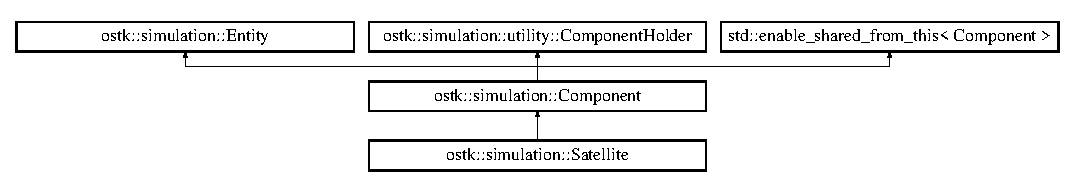
\includegraphics[height=2.066421cm]{classostk_1_1simulation_1_1_component}
\end{center}
\end{figure}
\subsection*{Public Types}
\begin{DoxyCompactItemize}
\item 
enum \hyperlink{classostk_1_1simulation_1_1_component_a1d2ded63a8ab0bd81e27f25921be1e20}{Type} \{ \newline
\hyperlink{classostk_1_1simulation_1_1_component_a1d2ded63a8ab0bd81e27f25921be1e20aec0fc0100c4fc1ce4eea230c3dc10360}{Type\+::\+Undefined}, 
\hyperlink{classostk_1_1simulation_1_1_component_a1d2ded63a8ab0bd81e27f25921be1e20ad75c45e11c8aeb13494dba59a388a164}{Type\+::\+Assembly}, 
\hyperlink{classostk_1_1simulation_1_1_component_a1d2ded63a8ab0bd81e27f25921be1e20a9bbf373797bf7cf7ba62c80023682e25}{Type\+::\+Controller}, 
\hyperlink{classostk_1_1simulation_1_1_component_a1d2ded63a8ab0bd81e27f25921be1e20a06b185256c71c1aec263c6e22bf8ef6b}{Type\+::\+Sensor}, 
\newline
\hyperlink{classostk_1_1simulation_1_1_component_a1d2ded63a8ab0bd81e27f25921be1e20aa2ec2ef7ebb614cf7dd5d78b9bbf59b3}{Type\+::\+Actuator}, 
\hyperlink{classostk_1_1simulation_1_1_component_a1d2ded63a8ab0bd81e27f25921be1e20a6311ae17c1ee52b36e68aaf4ad066387}{Type\+::\+Other}
 \}
\end{DoxyCompactItemize}
\subsection*{Public Member Functions}
\begin{DoxyCompactItemize}
\item 
\hyperlink{classostk_1_1simulation_1_1_component_ab3711f34980c3fdb746ff83b9511a25c}{Component} (const String \&an\+Id, const String \&a\+Name, const \hyperlink{classostk_1_1simulation_1_1_component_a1d2ded63a8ab0bd81e27f25921be1e20}{Component\+::\+Type} \&a\+Type, const Array$<$ String $>$ \&a\+Tag\+Array, const Array$<$ Shared$<$ \hyperlink{classostk_1_1simulation_1_1component_1_1_geometry}{Geometry} $>$$>$ \&a\+Geometry\+Array, const Array$<$ Shared$<$ \hyperlink{classostk_1_1simulation_1_1_component}{Component} $>$$>$ \&a\+Component\+Array, const Shared$<$ \hyperlink{classostk_1_1simulation_1_1utilities_1_1_component_holder}{Component\+Holder} $>$ \&a\+Parent\+Component\+S\+Ptr, const Shared$<$ const Frame $>$ \&a\+Frame\+S\+Ptr, const Shared$<$ const \hyperlink{classostk_1_1simulation_1_1_simulator}{Simulator} $>$ \&a\+Simulator\+S\+Ptr)
\item 
\hyperlink{classostk_1_1simulation_1_1_component_a5395700f491da619eb45b0148a5727d5}{Component} (const \hyperlink{classostk_1_1simulation_1_1_component}{Component} \&a\+Component)
\item 
virtual \hyperlink{classostk_1_1simulation_1_1_component_a57f790fdbb03f777e59d73218d2899ef}{$\sim$\+Component} ()
\item 
virtual \hyperlink{classostk_1_1simulation_1_1_component}{Component} $\ast$ \hyperlink{classostk_1_1simulation_1_1_component_a36cdd3498146b23e3ff67b95cd1c59cc}{clone} () const
\item 
bool \hyperlink{classostk_1_1simulation_1_1_component_a983ee8f3974fc2900f21d3bea12fb877}{is\+Defined} () const
\item 
const Shared$<$ const Frame $>$ \& \hyperlink{classostk_1_1simulation_1_1_component_a3e7acecda5a9286bc4baf1d3b6bbd7d5}{access\+Frame} () const
\item 
const \hyperlink{classostk_1_1simulation_1_1component_1_1_geometry}{Geometry} \& \hyperlink{classostk_1_1simulation_1_1_component_afe2d126a21b7a96d0b3655ebcac3a6be}{access\+Geometry\+With\+Name} (const String \&a\+Name) const
\item 
const \hyperlink{classostk_1_1simulation_1_1_simulator}{Simulator} \& \hyperlink{classostk_1_1simulation_1_1_component_a0e119aa1a610b08b935789a7ecb19605}{access\+Simulator} () const
\item 
\hyperlink{classostk_1_1simulation_1_1_component_a1d2ded63a8ab0bd81e27f25921be1e20}{Component\+::\+Type} \hyperlink{classostk_1_1simulation_1_1_component_a93375352059595b81e81569e445d4512}{get\+Type} () const
\item 
Array$<$ String $>$ \hyperlink{classostk_1_1simulation_1_1_component_ab792e508c303ec679ea8b8cbcc2c4c8f}{get\+Tags} () const
\item 
Array$<$ Shared$<$ \hyperlink{classostk_1_1simulation_1_1component_1_1_geometry}{Geometry} $>$ $>$ \hyperlink{classostk_1_1simulation_1_1_component_aba0796b346cbd27323c2e5c1df8ffcf2}{get\+Geometries} () const
\item 
void \hyperlink{classostk_1_1simulation_1_1_component_a266bf1a8b756f55ef24cc9fee3fd4fca}{set\+Parent} (const Shared$<$ \hyperlink{classostk_1_1simulation_1_1_component}{Component} $>$ \&a\+Component\+S\+Ptr)
\item 
void \hyperlink{classostk_1_1simulation_1_1_component_ad3ef491ef73a9e01507c95541790bdf2}{add\+Geometry} (const Shared$<$ \hyperlink{classostk_1_1simulation_1_1component_1_1_geometry}{Geometry} $>$ \&a\+Geometry\+S\+Ptr)
\item 
void \hyperlink{classostk_1_1simulation_1_1_component_aeb00ae625a59168bde62bcbb3e1d6ed6}{add\+Component} (const Shared$<$ \hyperlink{classostk_1_1simulation_1_1_component}{Component} $>$ \&a\+Component\+S\+Ptr)
\end{DoxyCompactItemize}
\subsection*{Static Public Member Functions}
\begin{DoxyCompactItemize}
\item 
static \hyperlink{classostk_1_1simulation_1_1_component}{Component} \hyperlink{classostk_1_1simulation_1_1_component_ad8849104db5f1e96a2de547bc1c11867}{Undefined} ()
\item 
static Shared$<$ \hyperlink{classostk_1_1simulation_1_1_component}{Component} $>$ \hyperlink{classostk_1_1simulation_1_1_component_a635e3685019800ec343ec8474954ff0e}{Configure} (const \hyperlink{structostk_1_1simulation_1_1_component_configuration}{Component\+Configuration} \&a\+Component\+Configuration, const Shared$<$ \hyperlink{classostk_1_1simulation_1_1_component}{Component} $>$ \&a\+Parent\+Component\+S\+Ptr)
\item 
static String \hyperlink{classostk_1_1simulation_1_1_component_a7f74a40eb3aae2f7e12af002ca9dbc89}{String\+From\+Type} (const \hyperlink{classostk_1_1simulation_1_1_component_a1d2ded63a8ab0bd81e27f25921be1e20}{Component\+::\+Type} \&a\+Type)
\item 
static Shared$<$ const Frame $>$ \hyperlink{classostk_1_1simulation_1_1_component_a9b5f84be02c06a7b6576fcdb00640ede}{Generate\+Frame} (const String \&a\+Name, const Quaternion \&a\+Quaternion, const Shared$<$ const Frame $>$ \&a\+Parent\+Frame\+S\+Ptr)
\end{DoxyCompactItemize}
\subsection*{Protected Member Functions}
\begin{DoxyCompactItemize}
\item 
virtual void \hyperlink{classostk_1_1simulation_1_1_component_a9c102937dd6ca5fb9e3b726cc0fd5ed6}{print} (std\+::ostream \&an\+Output\+Stream, bool display\+Decorators=true) const
\begin{DoxyCompactList}\small\item\em Print component. \end{DoxyCompactList}\end{DoxyCompactItemize}
\subsection*{Friends}
\begin{DoxyCompactItemize}
\item 
std\+::ostream \& \hyperlink{classostk_1_1simulation_1_1_component_ae3c657f10ed74f15e3356a2ff54647f3}{operator$<$$<$} (std\+::ostream \&an\+Output\+Stream, const \hyperlink{classostk_1_1simulation_1_1_component}{Component} \&a\+Component)
\end{DoxyCompactItemize}


\subsection{Detailed Description}
\hyperlink{classostk_1_1simulation_1_1_component}{Component}. 

\subsection{Member Enumeration Documentation}
\mbox{\Hypertarget{classostk_1_1simulation_1_1_component_a1d2ded63a8ab0bd81e27f25921be1e20}\label{classostk_1_1simulation_1_1_component_a1d2ded63a8ab0bd81e27f25921be1e20}} 
\index{ostk\+::simulation\+::\+Component@{ostk\+::simulation\+::\+Component}!Type@{Type}}
\index{Type@{Type}!ostk\+::simulation\+::\+Component@{ostk\+::simulation\+::\+Component}}
\subsubsection{\texorpdfstring{Type}{Type}}
{\footnotesize\ttfamily enum \hyperlink{classostk_1_1simulation_1_1_component_a1d2ded63a8ab0bd81e27f25921be1e20}{ostk\+::simulation\+::\+Component\+::\+Type}\hspace{0.3cm}{\ttfamily [strong]}}

\begin{DoxyEnumFields}{Enumerator}
\raisebox{\heightof{T}}[0pt][0pt]{\index{Undefined@{Undefined}!ostk\+::simulation\+::\+Component@{ostk\+::simulation\+::\+Component}}\index{ostk\+::simulation\+::\+Component@{ostk\+::simulation\+::\+Component}!Undefined@{Undefined}}}\mbox{\Hypertarget{classostk_1_1simulation_1_1_component_a1d2ded63a8ab0bd81e27f25921be1e20aec0fc0100c4fc1ce4eea230c3dc10360}\label{classostk_1_1simulation_1_1_component_a1d2ded63a8ab0bd81e27f25921be1e20aec0fc0100c4fc1ce4eea230c3dc10360}} 
Undefined&\\
\hline

\raisebox{\heightof{T}}[0pt][0pt]{\index{Assembly@{Assembly}!ostk\+::simulation\+::\+Component@{ostk\+::simulation\+::\+Component}}\index{ostk\+::simulation\+::\+Component@{ostk\+::simulation\+::\+Component}!Assembly@{Assembly}}}\mbox{\Hypertarget{classostk_1_1simulation_1_1_component_a1d2ded63a8ab0bd81e27f25921be1e20ad75c45e11c8aeb13494dba59a388a164}\label{classostk_1_1simulation_1_1_component_a1d2ded63a8ab0bd81e27f25921be1e20ad75c45e11c8aeb13494dba59a388a164}} 
Assembly&\\
\hline

\raisebox{\heightof{T}}[0pt][0pt]{\index{Controller@{Controller}!ostk\+::simulation\+::\+Component@{ostk\+::simulation\+::\+Component}}\index{ostk\+::simulation\+::\+Component@{ostk\+::simulation\+::\+Component}!Controller@{Controller}}}\mbox{\Hypertarget{classostk_1_1simulation_1_1_component_a1d2ded63a8ab0bd81e27f25921be1e20a9bbf373797bf7cf7ba62c80023682e25}\label{classostk_1_1simulation_1_1_component_a1d2ded63a8ab0bd81e27f25921be1e20a9bbf373797bf7cf7ba62c80023682e25}} 
Controller&\\
\hline

\raisebox{\heightof{T}}[0pt][0pt]{\index{Sensor@{Sensor}!ostk\+::simulation\+::\+Component@{ostk\+::simulation\+::\+Component}}\index{ostk\+::simulation\+::\+Component@{ostk\+::simulation\+::\+Component}!Sensor@{Sensor}}}\mbox{\Hypertarget{classostk_1_1simulation_1_1_component_a1d2ded63a8ab0bd81e27f25921be1e20a06b185256c71c1aec263c6e22bf8ef6b}\label{classostk_1_1simulation_1_1_component_a1d2ded63a8ab0bd81e27f25921be1e20a06b185256c71c1aec263c6e22bf8ef6b}} 
Sensor&\\
\hline

\raisebox{\heightof{T}}[0pt][0pt]{\index{Actuator@{Actuator}!ostk\+::simulation\+::\+Component@{ostk\+::simulation\+::\+Component}}\index{ostk\+::simulation\+::\+Component@{ostk\+::simulation\+::\+Component}!Actuator@{Actuator}}}\mbox{\Hypertarget{classostk_1_1simulation_1_1_component_a1d2ded63a8ab0bd81e27f25921be1e20aa2ec2ef7ebb614cf7dd5d78b9bbf59b3}\label{classostk_1_1simulation_1_1_component_a1d2ded63a8ab0bd81e27f25921be1e20aa2ec2ef7ebb614cf7dd5d78b9bbf59b3}} 
Actuator&\\
\hline

\raisebox{\heightof{T}}[0pt][0pt]{\index{Other@{Other}!ostk\+::simulation\+::\+Component@{ostk\+::simulation\+::\+Component}}\index{ostk\+::simulation\+::\+Component@{ostk\+::simulation\+::\+Component}!Other@{Other}}}\mbox{\Hypertarget{classostk_1_1simulation_1_1_component_a1d2ded63a8ab0bd81e27f25921be1e20a6311ae17c1ee52b36e68aaf4ad066387}\label{classostk_1_1simulation_1_1_component_a1d2ded63a8ab0bd81e27f25921be1e20a6311ae17c1ee52b36e68aaf4ad066387}} 
Other&\\
\hline

\end{DoxyEnumFields}


\subsection{Constructor \& Destructor Documentation}
\mbox{\Hypertarget{classostk_1_1simulation_1_1_component_ab3711f34980c3fdb746ff83b9511a25c}\label{classostk_1_1simulation_1_1_component_ab3711f34980c3fdb746ff83b9511a25c}} 
\index{ostk\+::simulation\+::\+Component@{ostk\+::simulation\+::\+Component}!Component@{Component}}
\index{Component@{Component}!ostk\+::simulation\+::\+Component@{ostk\+::simulation\+::\+Component}}
\subsubsection{\texorpdfstring{Component()}{Component()}\hspace{0.1cm}{\footnotesize\ttfamily [1/2]}}
{\footnotesize\ttfamily ostk\+::simulation\+::\+Component\+::\+Component (\begin{DoxyParamCaption}\item[{const String \&}]{an\+Id,  }\item[{const String \&}]{a\+Name,  }\item[{const \hyperlink{classostk_1_1simulation_1_1_component_a1d2ded63a8ab0bd81e27f25921be1e20}{Component\+::\+Type} \&}]{a\+Type,  }\item[{const Array$<$ String $>$ \&}]{a\+Tag\+Array,  }\item[{const Array$<$ Shared$<$ \hyperlink{classostk_1_1simulation_1_1component_1_1_geometry}{Geometry} $>$$>$ \&}]{a\+Geometry\+Array,  }\item[{const Array$<$ Shared$<$ \hyperlink{classostk_1_1simulation_1_1_component}{Component} $>$$>$ \&}]{a\+Component\+Array,  }\item[{const Shared$<$ \hyperlink{classostk_1_1simulation_1_1utilities_1_1_component_holder}{Component\+Holder} $>$ \&}]{a\+Parent\+Component\+S\+Ptr,  }\item[{const Shared$<$ const Frame $>$ \&}]{a\+Frame\+S\+Ptr,  }\item[{const Shared$<$ const \hyperlink{classostk_1_1simulation_1_1_simulator}{Simulator} $>$ \&}]{a\+Simulator\+S\+Ptr }\end{DoxyParamCaption})}

\mbox{\Hypertarget{classostk_1_1simulation_1_1_component_a5395700f491da619eb45b0148a5727d5}\label{classostk_1_1simulation_1_1_component_a5395700f491da619eb45b0148a5727d5}} 
\index{ostk\+::simulation\+::\+Component@{ostk\+::simulation\+::\+Component}!Component@{Component}}
\index{Component@{Component}!ostk\+::simulation\+::\+Component@{ostk\+::simulation\+::\+Component}}
\subsubsection{\texorpdfstring{Component()}{Component()}\hspace{0.1cm}{\footnotesize\ttfamily [2/2]}}
{\footnotesize\ttfamily ostk\+::simulation\+::\+Component\+::\+Component (\begin{DoxyParamCaption}\item[{const \hyperlink{classostk_1_1simulation_1_1_component}{Component} \&}]{a\+Component }\end{DoxyParamCaption})}

\mbox{\Hypertarget{classostk_1_1simulation_1_1_component_a57f790fdbb03f777e59d73218d2899ef}\label{classostk_1_1simulation_1_1_component_a57f790fdbb03f777e59d73218d2899ef}} 
\index{ostk\+::simulation\+::\+Component@{ostk\+::simulation\+::\+Component}!````~Component@{$\sim$\+Component}}
\index{````~Component@{$\sim$\+Component}!ostk\+::simulation\+::\+Component@{ostk\+::simulation\+::\+Component}}
\subsubsection{\texorpdfstring{$\sim$\+Component()}{~Component()}}
{\footnotesize\ttfamily ostk\+::simulation\+::\+Component\+::$\sim$\+Component (\begin{DoxyParamCaption}{ }\end{DoxyParamCaption})\hspace{0.3cm}{\ttfamily [virtual]}}



\subsection{Member Function Documentation}
\mbox{\Hypertarget{classostk_1_1simulation_1_1_component_a3e7acecda5a9286bc4baf1d3b6bbd7d5}\label{classostk_1_1simulation_1_1_component_a3e7acecda5a9286bc4baf1d3b6bbd7d5}} 
\index{ostk\+::simulation\+::\+Component@{ostk\+::simulation\+::\+Component}!access\+Frame@{access\+Frame}}
\index{access\+Frame@{access\+Frame}!ostk\+::simulation\+::\+Component@{ostk\+::simulation\+::\+Component}}
\subsubsection{\texorpdfstring{access\+Frame()}{accessFrame()}}
{\footnotesize\ttfamily const Shared$<$ const Frame $>$ \& ostk\+::simulation\+::\+Component\+::access\+Frame (\begin{DoxyParamCaption}{ }\end{DoxyParamCaption}) const}

\mbox{\Hypertarget{classostk_1_1simulation_1_1_component_afe2d126a21b7a96d0b3655ebcac3a6be}\label{classostk_1_1simulation_1_1_component_afe2d126a21b7a96d0b3655ebcac3a6be}} 
\index{ostk\+::simulation\+::\+Component@{ostk\+::simulation\+::\+Component}!access\+Geometry\+With\+Name@{access\+Geometry\+With\+Name}}
\index{access\+Geometry\+With\+Name@{access\+Geometry\+With\+Name}!ostk\+::simulation\+::\+Component@{ostk\+::simulation\+::\+Component}}
\subsubsection{\texorpdfstring{access\+Geometry\+With\+Name()}{accessGeometryWithName()}}
{\footnotesize\ttfamily const \hyperlink{classostk_1_1simulation_1_1component_1_1_geometry}{Geometry} \& ostk\+::simulation\+::\+Component\+::access\+Geometry\+With\+Name (\begin{DoxyParamCaption}\item[{const String \&}]{a\+Name }\end{DoxyParamCaption}) const}

\mbox{\Hypertarget{classostk_1_1simulation_1_1_component_a0e119aa1a610b08b935789a7ecb19605}\label{classostk_1_1simulation_1_1_component_a0e119aa1a610b08b935789a7ecb19605}} 
\index{ostk\+::simulation\+::\+Component@{ostk\+::simulation\+::\+Component}!access\+Simulator@{access\+Simulator}}
\index{access\+Simulator@{access\+Simulator}!ostk\+::simulation\+::\+Component@{ostk\+::simulation\+::\+Component}}
\subsubsection{\texorpdfstring{access\+Simulator()}{accessSimulator()}}
{\footnotesize\ttfamily const \hyperlink{classostk_1_1simulation_1_1_simulator}{Simulator} \& ostk\+::simulation\+::\+Component\+::access\+Simulator (\begin{DoxyParamCaption}{ }\end{DoxyParamCaption}) const}

\mbox{\Hypertarget{classostk_1_1simulation_1_1_component_aeb00ae625a59168bde62bcbb3e1d6ed6}\label{classostk_1_1simulation_1_1_component_aeb00ae625a59168bde62bcbb3e1d6ed6}} 
\index{ostk\+::simulation\+::\+Component@{ostk\+::simulation\+::\+Component}!add\+Component@{add\+Component}}
\index{add\+Component@{add\+Component}!ostk\+::simulation\+::\+Component@{ostk\+::simulation\+::\+Component}}
\subsubsection{\texorpdfstring{add\+Component()}{addComponent()}}
{\footnotesize\ttfamily void ostk\+::simulation\+::\+Component\+::add\+Component (\begin{DoxyParamCaption}\item[{const Shared$<$ \hyperlink{classostk_1_1simulation_1_1_component}{Component} $>$ \&}]{a\+Component\+S\+Ptr }\end{DoxyParamCaption})}

\mbox{\Hypertarget{classostk_1_1simulation_1_1_component_ad3ef491ef73a9e01507c95541790bdf2}\label{classostk_1_1simulation_1_1_component_ad3ef491ef73a9e01507c95541790bdf2}} 
\index{ostk\+::simulation\+::\+Component@{ostk\+::simulation\+::\+Component}!add\+Geometry@{add\+Geometry}}
\index{add\+Geometry@{add\+Geometry}!ostk\+::simulation\+::\+Component@{ostk\+::simulation\+::\+Component}}
\subsubsection{\texorpdfstring{add\+Geometry()}{addGeometry()}}
{\footnotesize\ttfamily void ostk\+::simulation\+::\+Component\+::add\+Geometry (\begin{DoxyParamCaption}\item[{const Shared$<$ \hyperlink{classostk_1_1simulation_1_1component_1_1_geometry}{Geometry} $>$ \&}]{a\+Geometry\+S\+Ptr }\end{DoxyParamCaption})}

\mbox{\Hypertarget{classostk_1_1simulation_1_1_component_a36cdd3498146b23e3ff67b95cd1c59cc}\label{classostk_1_1simulation_1_1_component_a36cdd3498146b23e3ff67b95cd1c59cc}} 
\index{ostk\+::simulation\+::\+Component@{ostk\+::simulation\+::\+Component}!clone@{clone}}
\index{clone@{clone}!ostk\+::simulation\+::\+Component@{ostk\+::simulation\+::\+Component}}
\subsubsection{\texorpdfstring{clone()}{clone()}}
{\footnotesize\ttfamily \hyperlink{classostk_1_1simulation_1_1_component}{Component} $\ast$ ostk\+::simulation\+::\+Component\+::clone (\begin{DoxyParamCaption}{ }\end{DoxyParamCaption}) const\hspace{0.3cm}{\ttfamily [virtual]}}



Reimplemented in \hyperlink{classostk_1_1simulation_1_1_satellite_a9828fe3ec02b8f4d8b2faf8412826f00}{ostk\+::simulation\+::\+Satellite}.

\mbox{\Hypertarget{classostk_1_1simulation_1_1_component_a635e3685019800ec343ec8474954ff0e}\label{classostk_1_1simulation_1_1_component_a635e3685019800ec343ec8474954ff0e}} 
\index{ostk\+::simulation\+::\+Component@{ostk\+::simulation\+::\+Component}!Configure@{Configure}}
\index{Configure@{Configure}!ostk\+::simulation\+::\+Component@{ostk\+::simulation\+::\+Component}}
\subsubsection{\texorpdfstring{Configure()}{Configure()}}
{\footnotesize\ttfamily Shared$<$ \hyperlink{classostk_1_1simulation_1_1_component}{Component} $>$ ostk\+::simulation\+::\+Component\+::\+Configure (\begin{DoxyParamCaption}\item[{const \hyperlink{structostk_1_1simulation_1_1_component_configuration}{Component\+Configuration} \&}]{a\+Component\+Configuration,  }\item[{const Shared$<$ \hyperlink{classostk_1_1simulation_1_1_component}{Component} $>$ \&}]{a\+Parent\+Component\+S\+Ptr }\end{DoxyParamCaption})\hspace{0.3cm}{\ttfamily [static]}}

\mbox{\Hypertarget{classostk_1_1simulation_1_1_component_a9b5f84be02c06a7b6576fcdb00640ede}\label{classostk_1_1simulation_1_1_component_a9b5f84be02c06a7b6576fcdb00640ede}} 
\index{ostk\+::simulation\+::\+Component@{ostk\+::simulation\+::\+Component}!Generate\+Frame@{Generate\+Frame}}
\index{Generate\+Frame@{Generate\+Frame}!ostk\+::simulation\+::\+Component@{ostk\+::simulation\+::\+Component}}
\subsubsection{\texorpdfstring{Generate\+Frame()}{GenerateFrame()}}
{\footnotesize\ttfamily Shared$<$ const Frame $>$ ostk\+::simulation\+::\+Component\+::\+Generate\+Frame (\begin{DoxyParamCaption}\item[{const String \&}]{a\+Name,  }\item[{const Quaternion \&}]{a\+Quaternion,  }\item[{const Shared$<$ const Frame $>$ \&}]{a\+Parent\+Frame\+S\+Ptr }\end{DoxyParamCaption})\hspace{0.3cm}{\ttfamily [static]}}

\mbox{\Hypertarget{classostk_1_1simulation_1_1_component_aba0796b346cbd27323c2e5c1df8ffcf2}\label{classostk_1_1simulation_1_1_component_aba0796b346cbd27323c2e5c1df8ffcf2}} 
\index{ostk\+::simulation\+::\+Component@{ostk\+::simulation\+::\+Component}!get\+Geometries@{get\+Geometries}}
\index{get\+Geometries@{get\+Geometries}!ostk\+::simulation\+::\+Component@{ostk\+::simulation\+::\+Component}}
\subsubsection{\texorpdfstring{get\+Geometries()}{getGeometries()}}
{\footnotesize\ttfamily Array$<$ Shared$<$ \hyperlink{classostk_1_1simulation_1_1component_1_1_geometry}{Geometry} $>$ $>$ ostk\+::simulation\+::\+Component\+::get\+Geometries (\begin{DoxyParamCaption}{ }\end{DoxyParamCaption}) const}

\mbox{\Hypertarget{classostk_1_1simulation_1_1_component_ab792e508c303ec679ea8b8cbcc2c4c8f}\label{classostk_1_1simulation_1_1_component_ab792e508c303ec679ea8b8cbcc2c4c8f}} 
\index{ostk\+::simulation\+::\+Component@{ostk\+::simulation\+::\+Component}!get\+Tags@{get\+Tags}}
\index{get\+Tags@{get\+Tags}!ostk\+::simulation\+::\+Component@{ostk\+::simulation\+::\+Component}}
\subsubsection{\texorpdfstring{get\+Tags()}{getTags()}}
{\footnotesize\ttfamily Array$<$ String $>$ ostk\+::simulation\+::\+Component\+::get\+Tags (\begin{DoxyParamCaption}{ }\end{DoxyParamCaption}) const}

\mbox{\Hypertarget{classostk_1_1simulation_1_1_component_a93375352059595b81e81569e445d4512}\label{classostk_1_1simulation_1_1_component_a93375352059595b81e81569e445d4512}} 
\index{ostk\+::simulation\+::\+Component@{ostk\+::simulation\+::\+Component}!get\+Type@{get\+Type}}
\index{get\+Type@{get\+Type}!ostk\+::simulation\+::\+Component@{ostk\+::simulation\+::\+Component}}
\subsubsection{\texorpdfstring{get\+Type()}{getType()}}
{\footnotesize\ttfamily \hyperlink{classostk_1_1simulation_1_1_component_a1d2ded63a8ab0bd81e27f25921be1e20}{Component\+::\+Type} ostk\+::simulation\+::\+Component\+::get\+Type (\begin{DoxyParamCaption}{ }\end{DoxyParamCaption}) const}

\mbox{\Hypertarget{classostk_1_1simulation_1_1_component_a983ee8f3974fc2900f21d3bea12fb877}\label{classostk_1_1simulation_1_1_component_a983ee8f3974fc2900f21d3bea12fb877}} 
\index{ostk\+::simulation\+::\+Component@{ostk\+::simulation\+::\+Component}!is\+Defined@{is\+Defined}}
\index{is\+Defined@{is\+Defined}!ostk\+::simulation\+::\+Component@{ostk\+::simulation\+::\+Component}}
\subsubsection{\texorpdfstring{is\+Defined()}{isDefined()}}
{\footnotesize\ttfamily bool ostk\+::simulation\+::\+Component\+::is\+Defined (\begin{DoxyParamCaption}{ }\end{DoxyParamCaption}) const}

\mbox{\Hypertarget{classostk_1_1simulation_1_1_component_a9c102937dd6ca5fb9e3b726cc0fd5ed6}\label{classostk_1_1simulation_1_1_component_a9c102937dd6ca5fb9e3b726cc0fd5ed6}} 
\index{ostk\+::simulation\+::\+Component@{ostk\+::simulation\+::\+Component}!print@{print}}
\index{print@{print}!ostk\+::simulation\+::\+Component@{ostk\+::simulation\+::\+Component}}
\subsubsection{\texorpdfstring{print()}{print()}}
{\footnotesize\ttfamily void ostk\+::simulation\+::\+Component\+::print (\begin{DoxyParamCaption}\item[{std\+::ostream \&}]{an\+Output\+Stream,  }\item[{bool}]{display\+Decorators = {\ttfamily true} }\end{DoxyParamCaption}) const\hspace{0.3cm}{\ttfamily [protected]}, {\ttfamily [virtual]}}



Print component. 


\begin{DoxyParams}[1]{Parameters}
\mbox{\tt in}  & {\em an\+Output\+Stream} & An output stream \\
\hline
\mbox{\tt in}  & {\em (optional)} & display\+Decorators If true, display decorators \\
\hline
\end{DoxyParams}


Reimplemented in \hyperlink{classostk_1_1simulation_1_1_satellite_ac7f5b5462deb081eb93115f0fb362acd}{ostk\+::simulation\+::\+Satellite}.

\mbox{\Hypertarget{classostk_1_1simulation_1_1_component_a266bf1a8b756f55ef24cc9fee3fd4fca}\label{classostk_1_1simulation_1_1_component_a266bf1a8b756f55ef24cc9fee3fd4fca}} 
\index{ostk\+::simulation\+::\+Component@{ostk\+::simulation\+::\+Component}!set\+Parent@{set\+Parent}}
\index{set\+Parent@{set\+Parent}!ostk\+::simulation\+::\+Component@{ostk\+::simulation\+::\+Component}}
\subsubsection{\texorpdfstring{set\+Parent()}{setParent()}}
{\footnotesize\ttfamily void ostk\+::simulation\+::\+Component\+::set\+Parent (\begin{DoxyParamCaption}\item[{const Shared$<$ \hyperlink{classostk_1_1simulation_1_1_component}{Component} $>$ \&}]{a\+Component\+S\+Ptr }\end{DoxyParamCaption})}

\mbox{\Hypertarget{classostk_1_1simulation_1_1_component_a7f74a40eb3aae2f7e12af002ca9dbc89}\label{classostk_1_1simulation_1_1_component_a7f74a40eb3aae2f7e12af002ca9dbc89}} 
\index{ostk\+::simulation\+::\+Component@{ostk\+::simulation\+::\+Component}!String\+From\+Type@{String\+From\+Type}}
\index{String\+From\+Type@{String\+From\+Type}!ostk\+::simulation\+::\+Component@{ostk\+::simulation\+::\+Component}}
\subsubsection{\texorpdfstring{String\+From\+Type()}{StringFromType()}}
{\footnotesize\ttfamily String ostk\+::simulation\+::\+Component\+::\+String\+From\+Type (\begin{DoxyParamCaption}\item[{const \hyperlink{classostk_1_1simulation_1_1_component_a1d2ded63a8ab0bd81e27f25921be1e20}{Component\+::\+Type} \&}]{a\+Type }\end{DoxyParamCaption})\hspace{0.3cm}{\ttfamily [static]}}

\mbox{\Hypertarget{classostk_1_1simulation_1_1_component_ad8849104db5f1e96a2de547bc1c11867}\label{classostk_1_1simulation_1_1_component_ad8849104db5f1e96a2de547bc1c11867}} 
\index{ostk\+::simulation\+::\+Component@{ostk\+::simulation\+::\+Component}!Undefined@{Undefined}}
\index{Undefined@{Undefined}!ostk\+::simulation\+::\+Component@{ostk\+::simulation\+::\+Component}}
\subsubsection{\texorpdfstring{Undefined()}{Undefined()}}
{\footnotesize\ttfamily \hyperlink{classostk_1_1simulation_1_1_component}{Component} ostk\+::simulation\+::\+Component\+::\+Undefined (\begin{DoxyParamCaption}{ }\end{DoxyParamCaption})\hspace{0.3cm}{\ttfamily [static]}}



\subsection{Friends And Related Function Documentation}
\mbox{\Hypertarget{classostk_1_1simulation_1_1_component_ae3c657f10ed74f15e3356a2ff54647f3}\label{classostk_1_1simulation_1_1_component_ae3c657f10ed74f15e3356a2ff54647f3}} 
\index{ostk\+::simulation\+::\+Component@{ostk\+::simulation\+::\+Component}!operator$<$$<$@{operator$<$$<$}}
\index{operator$<$$<$@{operator$<$$<$}!ostk\+::simulation\+::\+Component@{ostk\+::simulation\+::\+Component}}
\subsubsection{\texorpdfstring{operator$<$$<$}{operator<<}}
{\footnotesize\ttfamily std\+::ostream\& operator$<$$<$ (\begin{DoxyParamCaption}\item[{std\+::ostream \&}]{an\+Output\+Stream,  }\item[{const \hyperlink{classostk_1_1simulation_1_1_component}{Component} \&}]{a\+Component }\end{DoxyParamCaption})\hspace{0.3cm}{\ttfamily [friend]}}



The documentation for this class was generated from the following files\+:\begin{DoxyCompactItemize}
\item 
include/\+Open\+Space\+Toolkit/\+Simulation/\hyperlink{_component_8hpp}{Component.\+hpp}\item 
src/\+Open\+Space\+Toolkit/\+Simulation/\hyperlink{_component_8cpp}{Component.\+cpp}\end{DoxyCompactItemize}

\hypertarget{structostk_1_1simulation_1_1_component_configuration}{}\section{ostk\+:\+:simulation\+:\+:Component\+Configuration Struct Reference}
\label{structostk_1_1simulation_1_1_component_configuration}\index{ostk\+::simulation\+::\+Component\+Configuration@{ostk\+::simulation\+::\+Component\+Configuration}}


{\ttfamily \#include $<$Component.\+hpp$>$}

\subsection*{Public Attributes}
\begin{DoxyCompactItemize}
\item 
const String \hyperlink{structostk_1_1simulation_1_1_component_configuration_a7ef5e182de95028f8f50a45d2f36790a}{id}
\item 
const String \hyperlink{structostk_1_1simulation_1_1_component_configuration_ab78915c05378490b92166223f335b412}{name}
\item 
const \hyperlink{classostk_1_1simulation_1_1_component_a1d2ded63a8ab0bd81e27f25921be1e20}{Component\+::\+Type} \hyperlink{structostk_1_1simulation_1_1_component_configuration_abd0e836f95e58db5c8e954469101a2c8}{type} = \hyperlink{_component_8hpp_a0e5d3d0d9b45cdf8c94ed8df0d00c3e3}{D\+E\+F\+A\+U\+L\+T\+\_\+\+C\+O\+M\+P\+O\+N\+E\+N\+T\+\_\+\+T\+Y\+PE}
\item 
const Array$<$ String $>$ \hyperlink{structostk_1_1simulation_1_1_component_configuration_a95b38d1660657a8d2ba6baf0f885bf13}{tags} = \hyperlink{_satellite_8hpp_a7cabb8538f234177d4f95e681045bf94}{D\+E\+F\+A\+U\+L\+T\+\_\+\+T\+A\+GS}
\item 
const Quaternion \hyperlink{structostk_1_1simulation_1_1_component_configuration_a85c06b983a2aeddc726310ac64a280b6}{orientation} = \hyperlink{_component_8hpp_a5c684aeaeb24d197904b5a34839d2dd9}{D\+E\+F\+A\+U\+L\+T\+\_\+\+O\+R\+I\+E\+N\+T\+A\+T\+I\+ON}
\item 
const Array$<$ \hyperlink{structostk_1_1simulation_1_1component_1_1_geometry_configuration}{Geometry\+Configuration} $>$ \hyperlink{structostk_1_1simulation_1_1_component_configuration_a0b82a80f2def5a34efbb72697c6bc24e}{geometries} = \hyperlink{_satellite_8hpp_a4a68d11996a67b508045cdc894fac4ba}{D\+E\+F\+A\+U\+L\+T\+\_\+\+G\+E\+O\+M\+E\+T\+R\+I\+ES}
\item 
const Array$<$ \hyperlink{structostk_1_1simulation_1_1_component_configuration}{Component\+Configuration} $>$ \hyperlink{structostk_1_1simulation_1_1_component_configuration_aa6be134c476783e16aab75dc4b9e7b3d}{components} = \hyperlink{_satellite_8hpp_a4efe76b184101f122bb1be222cb65afc}{D\+E\+F\+A\+U\+L\+T\+\_\+\+C\+O\+M\+P\+O\+N\+E\+N\+TS}
\end{DoxyCompactItemize}


\subsection{Member Data Documentation}
\mbox{\Hypertarget{structostk_1_1simulation_1_1_component_configuration_aa6be134c476783e16aab75dc4b9e7b3d}\label{structostk_1_1simulation_1_1_component_configuration_aa6be134c476783e16aab75dc4b9e7b3d}} 
\index{ostk\+::simulation\+::\+Component\+Configuration@{ostk\+::simulation\+::\+Component\+Configuration}!components@{components}}
\index{components@{components}!ostk\+::simulation\+::\+Component\+Configuration@{ostk\+::simulation\+::\+Component\+Configuration}}
\subsubsection{\texorpdfstring{components}{components}}
{\footnotesize\ttfamily const Array$<$\hyperlink{structostk_1_1simulation_1_1_component_configuration}{Component\+Configuration}$>$ ostk\+::simulation\+::\+Component\+Configuration\+::components = \hyperlink{_satellite_8hpp_a4efe76b184101f122bb1be222cb65afc}{D\+E\+F\+A\+U\+L\+T\+\_\+\+C\+O\+M\+P\+O\+N\+E\+N\+TS}}

\mbox{\Hypertarget{structostk_1_1simulation_1_1_component_configuration_a0b82a80f2def5a34efbb72697c6bc24e}\label{structostk_1_1simulation_1_1_component_configuration_a0b82a80f2def5a34efbb72697c6bc24e}} 
\index{ostk\+::simulation\+::\+Component\+Configuration@{ostk\+::simulation\+::\+Component\+Configuration}!geometries@{geometries}}
\index{geometries@{geometries}!ostk\+::simulation\+::\+Component\+Configuration@{ostk\+::simulation\+::\+Component\+Configuration}}
\subsubsection{\texorpdfstring{geometries}{geometries}}
{\footnotesize\ttfamily const Array$<$\hyperlink{structostk_1_1simulation_1_1component_1_1_geometry_configuration}{Geometry\+Configuration}$>$ ostk\+::simulation\+::\+Component\+Configuration\+::geometries = \hyperlink{_satellite_8hpp_a4a68d11996a67b508045cdc894fac4ba}{D\+E\+F\+A\+U\+L\+T\+\_\+\+G\+E\+O\+M\+E\+T\+R\+I\+ES}}

\mbox{\Hypertarget{structostk_1_1simulation_1_1_component_configuration_a7ef5e182de95028f8f50a45d2f36790a}\label{structostk_1_1simulation_1_1_component_configuration_a7ef5e182de95028f8f50a45d2f36790a}} 
\index{ostk\+::simulation\+::\+Component\+Configuration@{ostk\+::simulation\+::\+Component\+Configuration}!id@{id}}
\index{id@{id}!ostk\+::simulation\+::\+Component\+Configuration@{ostk\+::simulation\+::\+Component\+Configuration}}
\subsubsection{\texorpdfstring{id}{id}}
{\footnotesize\ttfamily const String ostk\+::simulation\+::\+Component\+Configuration\+::id}

\mbox{\Hypertarget{structostk_1_1simulation_1_1_component_configuration_ab78915c05378490b92166223f335b412}\label{structostk_1_1simulation_1_1_component_configuration_ab78915c05378490b92166223f335b412}} 
\index{ostk\+::simulation\+::\+Component\+Configuration@{ostk\+::simulation\+::\+Component\+Configuration}!name@{name}}
\index{name@{name}!ostk\+::simulation\+::\+Component\+Configuration@{ostk\+::simulation\+::\+Component\+Configuration}}
\subsubsection{\texorpdfstring{name}{name}}
{\footnotesize\ttfamily const String ostk\+::simulation\+::\+Component\+Configuration\+::name}

\mbox{\Hypertarget{structostk_1_1simulation_1_1_component_configuration_a85c06b983a2aeddc726310ac64a280b6}\label{structostk_1_1simulation_1_1_component_configuration_a85c06b983a2aeddc726310ac64a280b6}} 
\index{ostk\+::simulation\+::\+Component\+Configuration@{ostk\+::simulation\+::\+Component\+Configuration}!orientation@{orientation}}
\index{orientation@{orientation}!ostk\+::simulation\+::\+Component\+Configuration@{ostk\+::simulation\+::\+Component\+Configuration}}
\subsubsection{\texorpdfstring{orientation}{orientation}}
{\footnotesize\ttfamily const Quaternion ostk\+::simulation\+::\+Component\+Configuration\+::orientation = \hyperlink{_component_8hpp_a5c684aeaeb24d197904b5a34839d2dd9}{D\+E\+F\+A\+U\+L\+T\+\_\+\+O\+R\+I\+E\+N\+T\+A\+T\+I\+ON}}

\mbox{\Hypertarget{structostk_1_1simulation_1_1_component_configuration_a95b38d1660657a8d2ba6baf0f885bf13}\label{structostk_1_1simulation_1_1_component_configuration_a95b38d1660657a8d2ba6baf0f885bf13}} 
\index{ostk\+::simulation\+::\+Component\+Configuration@{ostk\+::simulation\+::\+Component\+Configuration}!tags@{tags}}
\index{tags@{tags}!ostk\+::simulation\+::\+Component\+Configuration@{ostk\+::simulation\+::\+Component\+Configuration}}
\subsubsection{\texorpdfstring{tags}{tags}}
{\footnotesize\ttfamily const Array$<$String$>$ ostk\+::simulation\+::\+Component\+Configuration\+::tags = \hyperlink{_satellite_8hpp_a7cabb8538f234177d4f95e681045bf94}{D\+E\+F\+A\+U\+L\+T\+\_\+\+T\+A\+GS}}

\mbox{\Hypertarget{structostk_1_1simulation_1_1_component_configuration_abd0e836f95e58db5c8e954469101a2c8}\label{structostk_1_1simulation_1_1_component_configuration_abd0e836f95e58db5c8e954469101a2c8}} 
\index{ostk\+::simulation\+::\+Component\+Configuration@{ostk\+::simulation\+::\+Component\+Configuration}!type@{type}}
\index{type@{type}!ostk\+::simulation\+::\+Component\+Configuration@{ostk\+::simulation\+::\+Component\+Configuration}}
\subsubsection{\texorpdfstring{type}{type}}
{\footnotesize\ttfamily const \hyperlink{classostk_1_1simulation_1_1_component_a1d2ded63a8ab0bd81e27f25921be1e20}{Component\+::\+Type} ostk\+::simulation\+::\+Component\+Configuration\+::type = \hyperlink{_component_8hpp_a0e5d3d0d9b45cdf8c94ed8df0d00c3e3}{D\+E\+F\+A\+U\+L\+T\+\_\+\+C\+O\+M\+P\+O\+N\+E\+N\+T\+\_\+\+T\+Y\+PE}}



The documentation for this struct was generated from the following file\+:\begin{DoxyCompactItemize}
\item 
include/\+Open\+Space\+Toolkit/\+Simulation/\hyperlink{_component_8hpp}{Component.\+hpp}\end{DoxyCompactItemize}

\hypertarget{classostk_1_1simulation_1_1utilities_1_1_component_holder}{}\doxysection{ostk\+::simulation\+::utilities\+::Component\+Holder Class Reference}
\label{classostk_1_1simulation_1_1utilities_1_1_component_holder}\index{ostk::simulation::utilities::ComponentHolder@{ostk::simulation::utilities::ComponentHolder}}


Generic \mbox{\hyperlink{classostk_1_1simulation_1_1_component}{Component}} holder.  




{\ttfamily \#include $<$Component\+Holder.\+hpp$>$}

Inheritance diagram for ostk\+::simulation\+::utilities\+::Component\+Holder\+:\begin{figure}[H]
\begin{center}
\leavevmode
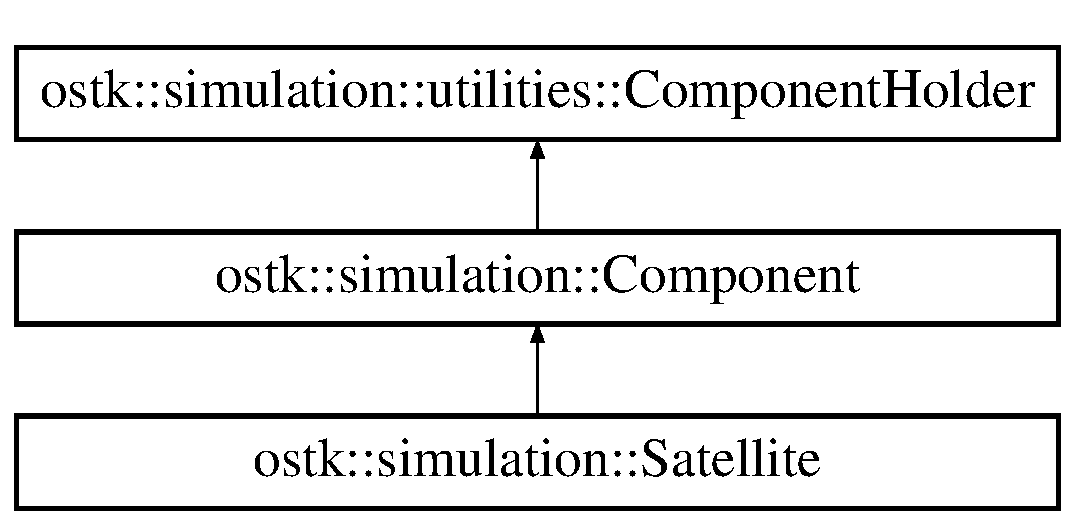
\includegraphics[height=3.000000cm]{classostk_1_1simulation_1_1utilities_1_1_component_holder}
\end{center}
\end{figure}
\doxysubsection*{Public Member Functions}
\begin{DoxyCompactItemize}
\item 
\mbox{\hyperlink{classostk_1_1simulation_1_1utilities_1_1_component_holder_a8c55b3d1233adaa5363893de07b44c40}{Component\+Holder}} (const Array$<$ Shared$<$ \mbox{\hyperlink{classostk_1_1simulation_1_1_component}{Component}} $>$$>$ \&a\+Component\+Array=Array$<$ Shared$<$ \mbox{\hyperlink{classostk_1_1simulation_1_1_component}{Component}} $>$$>$\+::Empty())
\item 
\mbox{\hyperlink{classostk_1_1simulation_1_1utilities_1_1_component_holder_a62afb2161daf9f4dba0a02c2cd1d644d}{Component\+Holder}} (const \mbox{\hyperlink{classostk_1_1simulation_1_1utilities_1_1_component_holder}{Component\+Holder}} \&a\+Component\+Holder)
\item 
\mbox{\hyperlink{classostk_1_1simulation_1_1utilities_1_1_component_holder_ad0adf394f0c30d64e5ccbf7638802b02}{$\sim$\+Component\+Holder}} ()
\item 
bool \mbox{\hyperlink{classostk_1_1simulation_1_1utilities_1_1_component_holder_a401459c4bd2606f6e15c4af732240e6b}{has\+Component\+With\+Id}} (const String \&a\+Component\+Id) const
\item 
bool \mbox{\hyperlink{classostk_1_1simulation_1_1utilities_1_1_component_holder_a74f0c97edae7bd4e8cf626749374aa3b}{has\+Component\+With\+Name}} (const String \&a\+Component\+Name) const
\item 
bool \mbox{\hyperlink{classostk_1_1simulation_1_1utilities_1_1_component_holder_ac8f363b3946caf1afbc6278931a9d764}{has\+Component\+At}} (const String \&a\+Component\+Path) const
\item 
Array$<$ Shared$<$ \mbox{\hyperlink{classostk_1_1simulation_1_1_component}{Component}} $>$ $>$ \mbox{\hyperlink{classostk_1_1simulation_1_1utilities_1_1_component_holder_a71d4e98af453e82bf1257d926b29fe78}{access\+Components}} () const
\item 
const \mbox{\hyperlink{classostk_1_1simulation_1_1_component}{Component}} \& \mbox{\hyperlink{classostk_1_1simulation_1_1utilities_1_1_component_holder_ad3f8b1059d3e41ce87c6916f0e2efb71}{access\+Component\+With\+Id}} (const String \&a\+Component\+Id) const
\item 
const \mbox{\hyperlink{classostk_1_1simulation_1_1_component}{Component}} \& \mbox{\hyperlink{classostk_1_1simulation_1_1utilities_1_1_component_holder_a5ebd352bbc6031ff288106be9e4cc4c8}{access\+Component\+With\+Name}} (const String \&a\+Component\+Name) const
\item 
Array$<$ Shared$<$ const \mbox{\hyperlink{classostk_1_1simulation_1_1_component}{Component}} $>$ $>$ \mbox{\hyperlink{classostk_1_1simulation_1_1utilities_1_1_component_holder_a8dd785dcaa575278edd76cd14a245e1d}{access\+Components\+With\+Tag}} (const String \&a\+Component\+Tag) const
\item 
const \mbox{\hyperlink{classostk_1_1simulation_1_1_component}{Component}} \& \mbox{\hyperlink{classostk_1_1simulation_1_1utilities_1_1_component_holder_a0ab33e5a3ae44d8be3690f56a7780951}{access\+Component\+At}} (const String \&a\+Component\+Path) const
\item 
void \mbox{\hyperlink{classostk_1_1simulation_1_1utilities_1_1_component_holder_a6126f9412580307762b172837ecfd469}{add\+Component}} (const Shared$<$ \mbox{\hyperlink{classostk_1_1simulation_1_1_component}{Component}} $>$ \&a\+Component\+S\+Ptr)
\end{DoxyCompactItemize}


\doxysubsection{Detailed Description}
Generic \mbox{\hyperlink{classostk_1_1simulation_1_1_component}{Component}} holder. 

\doxysubsection{Constructor \& Destructor Documentation}
\mbox{\Hypertarget{classostk_1_1simulation_1_1utilities_1_1_component_holder_a8c55b3d1233adaa5363893de07b44c40}\label{classostk_1_1simulation_1_1utilities_1_1_component_holder_a8c55b3d1233adaa5363893de07b44c40}} 
\index{ostk::simulation::utilities::ComponentHolder@{ostk::simulation::utilities::ComponentHolder}!ComponentHolder@{ComponentHolder}}
\index{ComponentHolder@{ComponentHolder}!ostk::simulation::utilities::ComponentHolder@{ostk::simulation::utilities::ComponentHolder}}
\doxysubsubsection{\texorpdfstring{ComponentHolder()}{ComponentHolder()}\hspace{0.1cm}{\footnotesize\ttfamily [1/2]}}
{\footnotesize\ttfamily ostk\+::simulation\+::utilities\+::\+Component\+Holder\+::\+Component\+Holder (\begin{DoxyParamCaption}\item[{const Array$<$ Shared$<$ \mbox{\hyperlink{classostk_1_1simulation_1_1_component}{Component}} $>$$>$ \&}]{a\+Component\+Array = {\ttfamily Array$<$Shared$<$\mbox{\hyperlink{classostk_1_1simulation_1_1_component}{Component}}$>$$>$\+:\+:Empty()} }\end{DoxyParamCaption})}

\mbox{\Hypertarget{classostk_1_1simulation_1_1utilities_1_1_component_holder_a62afb2161daf9f4dba0a02c2cd1d644d}\label{classostk_1_1simulation_1_1utilities_1_1_component_holder_a62afb2161daf9f4dba0a02c2cd1d644d}} 
\index{ostk::simulation::utilities::ComponentHolder@{ostk::simulation::utilities::ComponentHolder}!ComponentHolder@{ComponentHolder}}
\index{ComponentHolder@{ComponentHolder}!ostk::simulation::utilities::ComponentHolder@{ostk::simulation::utilities::ComponentHolder}}
\doxysubsubsection{\texorpdfstring{ComponentHolder()}{ComponentHolder()}\hspace{0.1cm}{\footnotesize\ttfamily [2/2]}}
{\footnotesize\ttfamily ostk\+::simulation\+::utilities\+::\+Component\+Holder\+::\+Component\+Holder (\begin{DoxyParamCaption}\item[{const \mbox{\hyperlink{classostk_1_1simulation_1_1utilities_1_1_component_holder}{Component\+Holder}} \&}]{a\+Component\+Holder }\end{DoxyParamCaption})}

\mbox{\Hypertarget{classostk_1_1simulation_1_1utilities_1_1_component_holder_ad0adf394f0c30d64e5ccbf7638802b02}\label{classostk_1_1simulation_1_1utilities_1_1_component_holder_ad0adf394f0c30d64e5ccbf7638802b02}} 
\index{ostk::simulation::utilities::ComponentHolder@{ostk::simulation::utilities::ComponentHolder}!````~ComponentHolder@{$\sim$ComponentHolder}}
\index{````~ComponentHolder@{$\sim$ComponentHolder}!ostk::simulation::utilities::ComponentHolder@{ostk::simulation::utilities::ComponentHolder}}
\doxysubsubsection{\texorpdfstring{$\sim$ComponentHolder()}{~ComponentHolder()}}
{\footnotesize\ttfamily ostk\+::simulation\+::utilities\+::\+Component\+Holder\+::$\sim$\+Component\+Holder (\begin{DoxyParamCaption}{ }\end{DoxyParamCaption})}



\doxysubsection{Member Function Documentation}
\mbox{\Hypertarget{classostk_1_1simulation_1_1utilities_1_1_component_holder_a0ab33e5a3ae44d8be3690f56a7780951}\label{classostk_1_1simulation_1_1utilities_1_1_component_holder_a0ab33e5a3ae44d8be3690f56a7780951}} 
\index{ostk::simulation::utilities::ComponentHolder@{ostk::simulation::utilities::ComponentHolder}!accessComponentAt@{accessComponentAt}}
\index{accessComponentAt@{accessComponentAt}!ostk::simulation::utilities::ComponentHolder@{ostk::simulation::utilities::ComponentHolder}}
\doxysubsubsection{\texorpdfstring{accessComponentAt()}{accessComponentAt()}}
{\footnotesize\ttfamily const \mbox{\hyperlink{classostk_1_1simulation_1_1_component}{Component}} \& ostk\+::simulation\+::utilities\+::\+Component\+Holder\+::access\+Component\+At (\begin{DoxyParamCaption}\item[{const String \&}]{a\+Component\+Path }\end{DoxyParamCaption}) const}

\mbox{\Hypertarget{classostk_1_1simulation_1_1utilities_1_1_component_holder_a71d4e98af453e82bf1257d926b29fe78}\label{classostk_1_1simulation_1_1utilities_1_1_component_holder_a71d4e98af453e82bf1257d926b29fe78}} 
\index{ostk::simulation::utilities::ComponentHolder@{ostk::simulation::utilities::ComponentHolder}!accessComponents@{accessComponents}}
\index{accessComponents@{accessComponents}!ostk::simulation::utilities::ComponentHolder@{ostk::simulation::utilities::ComponentHolder}}
\doxysubsubsection{\texorpdfstring{accessComponents()}{accessComponents()}}
{\footnotesize\ttfamily Array$<$ Shared$<$ \mbox{\hyperlink{classostk_1_1simulation_1_1_component}{Component}} $>$ $>$ ostk\+::simulation\+::utilities\+::\+Component\+Holder\+::access\+Components (\begin{DoxyParamCaption}{ }\end{DoxyParamCaption}) const}

\mbox{\Hypertarget{classostk_1_1simulation_1_1utilities_1_1_component_holder_a8dd785dcaa575278edd76cd14a245e1d}\label{classostk_1_1simulation_1_1utilities_1_1_component_holder_a8dd785dcaa575278edd76cd14a245e1d}} 
\index{ostk::simulation::utilities::ComponentHolder@{ostk::simulation::utilities::ComponentHolder}!accessComponentsWithTag@{accessComponentsWithTag}}
\index{accessComponentsWithTag@{accessComponentsWithTag}!ostk::simulation::utilities::ComponentHolder@{ostk::simulation::utilities::ComponentHolder}}
\doxysubsubsection{\texorpdfstring{accessComponentsWithTag()}{accessComponentsWithTag()}}
{\footnotesize\ttfamily Array$<$ Shared$<$ const \mbox{\hyperlink{classostk_1_1simulation_1_1_component}{Component}} $>$ $>$ ostk\+::simulation\+::utilities\+::\+Component\+Holder\+::access\+Components\+With\+Tag (\begin{DoxyParamCaption}\item[{const String \&}]{a\+Component\+Tag }\end{DoxyParamCaption}) const}

\mbox{\Hypertarget{classostk_1_1simulation_1_1utilities_1_1_component_holder_ad3f8b1059d3e41ce87c6916f0e2efb71}\label{classostk_1_1simulation_1_1utilities_1_1_component_holder_ad3f8b1059d3e41ce87c6916f0e2efb71}} 
\index{ostk::simulation::utilities::ComponentHolder@{ostk::simulation::utilities::ComponentHolder}!accessComponentWithId@{accessComponentWithId}}
\index{accessComponentWithId@{accessComponentWithId}!ostk::simulation::utilities::ComponentHolder@{ostk::simulation::utilities::ComponentHolder}}
\doxysubsubsection{\texorpdfstring{accessComponentWithId()}{accessComponentWithId()}}
{\footnotesize\ttfamily const \mbox{\hyperlink{classostk_1_1simulation_1_1_component}{Component}} \& ostk\+::simulation\+::utilities\+::\+Component\+Holder\+::access\+Component\+With\+Id (\begin{DoxyParamCaption}\item[{const String \&}]{a\+Component\+Id }\end{DoxyParamCaption}) const}

\mbox{\Hypertarget{classostk_1_1simulation_1_1utilities_1_1_component_holder_a5ebd352bbc6031ff288106be9e4cc4c8}\label{classostk_1_1simulation_1_1utilities_1_1_component_holder_a5ebd352bbc6031ff288106be9e4cc4c8}} 
\index{ostk::simulation::utilities::ComponentHolder@{ostk::simulation::utilities::ComponentHolder}!accessComponentWithName@{accessComponentWithName}}
\index{accessComponentWithName@{accessComponentWithName}!ostk::simulation::utilities::ComponentHolder@{ostk::simulation::utilities::ComponentHolder}}
\doxysubsubsection{\texorpdfstring{accessComponentWithName()}{accessComponentWithName()}}
{\footnotesize\ttfamily const \mbox{\hyperlink{classostk_1_1simulation_1_1_component}{Component}} \& ostk\+::simulation\+::utilities\+::\+Component\+Holder\+::access\+Component\+With\+Name (\begin{DoxyParamCaption}\item[{const String \&}]{a\+Component\+Name }\end{DoxyParamCaption}) const}

\mbox{\Hypertarget{classostk_1_1simulation_1_1utilities_1_1_component_holder_a6126f9412580307762b172837ecfd469}\label{classostk_1_1simulation_1_1utilities_1_1_component_holder_a6126f9412580307762b172837ecfd469}} 
\index{ostk::simulation::utilities::ComponentHolder@{ostk::simulation::utilities::ComponentHolder}!addComponent@{addComponent}}
\index{addComponent@{addComponent}!ostk::simulation::utilities::ComponentHolder@{ostk::simulation::utilities::ComponentHolder}}
\doxysubsubsection{\texorpdfstring{addComponent()}{addComponent()}}
{\footnotesize\ttfamily void ostk\+::simulation\+::utilities\+::\+Component\+Holder\+::add\+Component (\begin{DoxyParamCaption}\item[{const Shared$<$ \mbox{\hyperlink{classostk_1_1simulation_1_1_component}{Component}} $>$ \&}]{a\+Component\+S\+Ptr }\end{DoxyParamCaption})}

\mbox{\Hypertarget{classostk_1_1simulation_1_1utilities_1_1_component_holder_ac8f363b3946caf1afbc6278931a9d764}\label{classostk_1_1simulation_1_1utilities_1_1_component_holder_ac8f363b3946caf1afbc6278931a9d764}} 
\index{ostk::simulation::utilities::ComponentHolder@{ostk::simulation::utilities::ComponentHolder}!hasComponentAt@{hasComponentAt}}
\index{hasComponentAt@{hasComponentAt}!ostk::simulation::utilities::ComponentHolder@{ostk::simulation::utilities::ComponentHolder}}
\doxysubsubsection{\texorpdfstring{hasComponentAt()}{hasComponentAt()}}
{\footnotesize\ttfamily bool ostk\+::simulation\+::utilities\+::\+Component\+Holder\+::has\+Component\+At (\begin{DoxyParamCaption}\item[{const String \&}]{a\+Component\+Path }\end{DoxyParamCaption}) const}

\mbox{\Hypertarget{classostk_1_1simulation_1_1utilities_1_1_component_holder_a401459c4bd2606f6e15c4af732240e6b}\label{classostk_1_1simulation_1_1utilities_1_1_component_holder_a401459c4bd2606f6e15c4af732240e6b}} 
\index{ostk::simulation::utilities::ComponentHolder@{ostk::simulation::utilities::ComponentHolder}!hasComponentWithId@{hasComponentWithId}}
\index{hasComponentWithId@{hasComponentWithId}!ostk::simulation::utilities::ComponentHolder@{ostk::simulation::utilities::ComponentHolder}}
\doxysubsubsection{\texorpdfstring{hasComponentWithId()}{hasComponentWithId()}}
{\footnotesize\ttfamily bool ostk\+::simulation\+::utilities\+::\+Component\+Holder\+::has\+Component\+With\+Id (\begin{DoxyParamCaption}\item[{const String \&}]{a\+Component\+Id }\end{DoxyParamCaption}) const}

\mbox{\Hypertarget{classostk_1_1simulation_1_1utilities_1_1_component_holder_a74f0c97edae7bd4e8cf626749374aa3b}\label{classostk_1_1simulation_1_1utilities_1_1_component_holder_a74f0c97edae7bd4e8cf626749374aa3b}} 
\index{ostk::simulation::utilities::ComponentHolder@{ostk::simulation::utilities::ComponentHolder}!hasComponentWithName@{hasComponentWithName}}
\index{hasComponentWithName@{hasComponentWithName}!ostk::simulation::utilities::ComponentHolder@{ostk::simulation::utilities::ComponentHolder}}
\doxysubsubsection{\texorpdfstring{hasComponentWithName()}{hasComponentWithName()}}
{\footnotesize\ttfamily bool ostk\+::simulation\+::utilities\+::\+Component\+Holder\+::has\+Component\+With\+Name (\begin{DoxyParamCaption}\item[{const String \&}]{a\+Component\+Name }\end{DoxyParamCaption}) const}



The documentation for this class was generated from the following files\+:\begin{DoxyCompactItemize}
\item 
include/\+Open\+Space\+Toolkit/\+Simulation/\+Utilities/\mbox{\hyperlink{_component_holder_8hpp}{Component\+Holder.\+hpp}}\item 
src/\+Open\+Space\+Toolkit/\+Simulation/\+Utilities/\mbox{\hyperlink{_component_holder_8cpp}{Component\+Holder.\+cpp}}\end{DoxyCompactItemize}

\hypertarget{classostk_1_1simulation_1_1_entity}{}\doxysection{ostk\+::simulation\+::Entity Class Reference}
\label{classostk_1_1simulation_1_1_entity}\index{ostk::simulation::Entity@{ostk::simulation::Entity}}


\mbox{\hyperlink{classostk_1_1simulation_1_1_entity}{Entity}}.  




{\ttfamily \#include $<$Entity.\+hpp$>$}

Inheritance diagram for ostk\+::simulation\+::Entity\+:\begin{figure}[H]
\begin{center}
\leavevmode
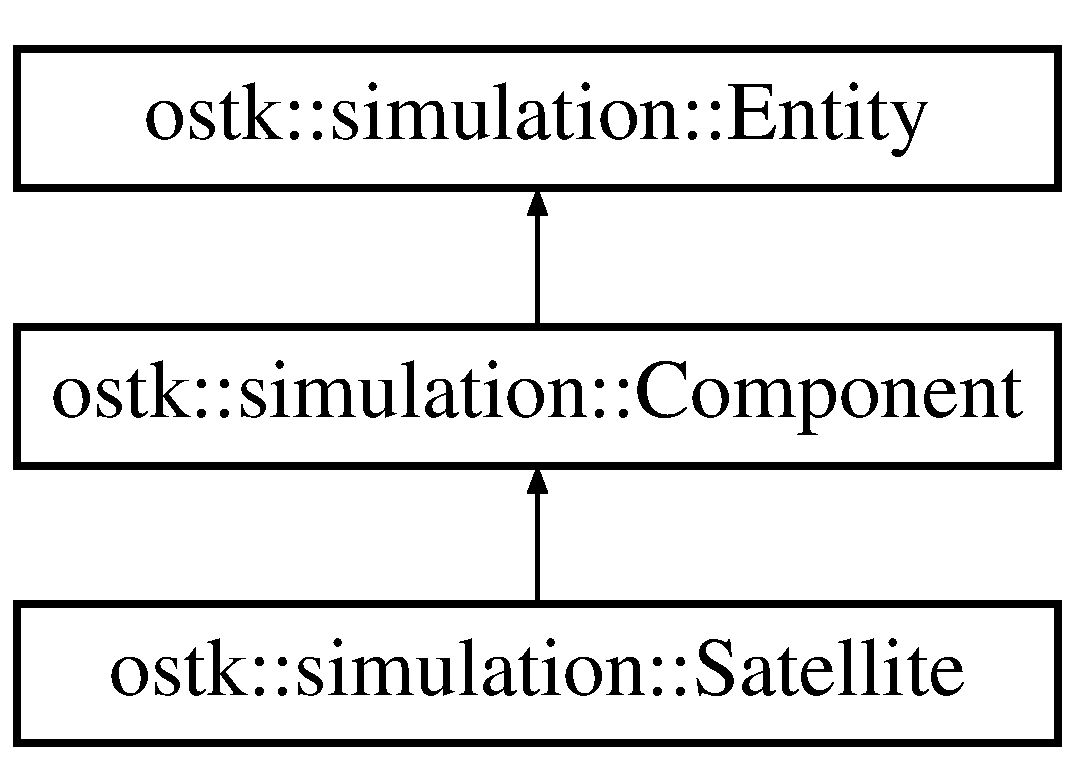
\includegraphics[height=3.000000cm]{classostk_1_1simulation_1_1_entity}
\end{center}
\end{figure}
\doxysubsection*{Public Member Functions}
\begin{DoxyCompactItemize}
\item 
\mbox{\hyperlink{classostk_1_1simulation_1_1_entity_a929819736161db5935b29b84da8a97aa}{Entity}} (const String \&a\+Name)
\item 
\mbox{\hyperlink{classostk_1_1simulation_1_1_entity_ae4ee439011cfcb1811d31bdb8db871fa}{Entity}} (const String \&an\+Id, const String \&a\+Name)
\item 
bool \mbox{\hyperlink{classostk_1_1simulation_1_1_entity_ad3c1556400b02acdffde053348acda2f}{is\+Defined}} () const
\item 
String \mbox{\hyperlink{classostk_1_1simulation_1_1_entity_a33286b8807aacec430d105646c021a79}{get\+Id}} () const
\item 
String \mbox{\hyperlink{classostk_1_1simulation_1_1_entity_a17050a1483e16e62ca10e3b1ecade1d5}{get\+Name}} () const
\item 
void \mbox{\hyperlink{classostk_1_1simulation_1_1_entity_aa2238f2fe07b5ddc4594293acdfa0c23}{print}} (std\+::ostream \&an\+Output\+Stream, bool display\+Decorators=true) const
\begin{DoxyCompactList}\small\item\em Print entity. \end{DoxyCompactList}\end{DoxyCompactItemize}
\doxysubsection*{Static Public Member Functions}
\begin{DoxyCompactItemize}
\item 
static \mbox{\hyperlink{classostk_1_1simulation_1_1_entity}{Entity}} \mbox{\hyperlink{classostk_1_1simulation_1_1_entity_aa42c610f1b96197f9fbf45711fe6a479}{Undefined}} ()
\end{DoxyCompactItemize}


\doxysubsection{Detailed Description}
\mbox{\hyperlink{classostk_1_1simulation_1_1_entity}{Entity}}. 

\doxysubsection{Constructor \& Destructor Documentation}
\mbox{\Hypertarget{classostk_1_1simulation_1_1_entity_a929819736161db5935b29b84da8a97aa}\label{classostk_1_1simulation_1_1_entity_a929819736161db5935b29b84da8a97aa}} 
\index{ostk::simulation::Entity@{ostk::simulation::Entity}!Entity@{Entity}}
\index{Entity@{Entity}!ostk::simulation::Entity@{ostk::simulation::Entity}}
\doxysubsubsection{\texorpdfstring{Entity()}{Entity()}\hspace{0.1cm}{\footnotesize\ttfamily [1/2]}}
{\footnotesize\ttfamily ostk\+::simulation\+::\+Entity\+::\+Entity (\begin{DoxyParamCaption}\item[{const String \&}]{a\+Name }\end{DoxyParamCaption})}

\mbox{\Hypertarget{classostk_1_1simulation_1_1_entity_ae4ee439011cfcb1811d31bdb8db871fa}\label{classostk_1_1simulation_1_1_entity_ae4ee439011cfcb1811d31bdb8db871fa}} 
\index{ostk::simulation::Entity@{ostk::simulation::Entity}!Entity@{Entity}}
\index{Entity@{Entity}!ostk::simulation::Entity@{ostk::simulation::Entity}}
\doxysubsubsection{\texorpdfstring{Entity()}{Entity()}\hspace{0.1cm}{\footnotesize\ttfamily [2/2]}}
{\footnotesize\ttfamily ostk\+::simulation\+::\+Entity\+::\+Entity (\begin{DoxyParamCaption}\item[{const String \&}]{an\+Id,  }\item[{const String \&}]{a\+Name }\end{DoxyParamCaption})}



\doxysubsection{Member Function Documentation}
\mbox{\Hypertarget{classostk_1_1simulation_1_1_entity_a33286b8807aacec430d105646c021a79}\label{classostk_1_1simulation_1_1_entity_a33286b8807aacec430d105646c021a79}} 
\index{ostk::simulation::Entity@{ostk::simulation::Entity}!getId@{getId}}
\index{getId@{getId}!ostk::simulation::Entity@{ostk::simulation::Entity}}
\doxysubsubsection{\texorpdfstring{getId()}{getId()}}
{\footnotesize\ttfamily String ostk\+::simulation\+::\+Entity\+::get\+Id (\begin{DoxyParamCaption}{ }\end{DoxyParamCaption}) const}

\mbox{\Hypertarget{classostk_1_1simulation_1_1_entity_a17050a1483e16e62ca10e3b1ecade1d5}\label{classostk_1_1simulation_1_1_entity_a17050a1483e16e62ca10e3b1ecade1d5}} 
\index{ostk::simulation::Entity@{ostk::simulation::Entity}!getName@{getName}}
\index{getName@{getName}!ostk::simulation::Entity@{ostk::simulation::Entity}}
\doxysubsubsection{\texorpdfstring{getName()}{getName()}}
{\footnotesize\ttfamily String ostk\+::simulation\+::\+Entity\+::get\+Name (\begin{DoxyParamCaption}{ }\end{DoxyParamCaption}) const}

\mbox{\Hypertarget{classostk_1_1simulation_1_1_entity_ad3c1556400b02acdffde053348acda2f}\label{classostk_1_1simulation_1_1_entity_ad3c1556400b02acdffde053348acda2f}} 
\index{ostk::simulation::Entity@{ostk::simulation::Entity}!isDefined@{isDefined}}
\index{isDefined@{isDefined}!ostk::simulation::Entity@{ostk::simulation::Entity}}
\doxysubsubsection{\texorpdfstring{isDefined()}{isDefined()}}
{\footnotesize\ttfamily bool ostk\+::simulation\+::\+Entity\+::is\+Defined (\begin{DoxyParamCaption}{ }\end{DoxyParamCaption}) const}

\mbox{\Hypertarget{classostk_1_1simulation_1_1_entity_aa2238f2fe07b5ddc4594293acdfa0c23}\label{classostk_1_1simulation_1_1_entity_aa2238f2fe07b5ddc4594293acdfa0c23}} 
\index{ostk::simulation::Entity@{ostk::simulation::Entity}!print@{print}}
\index{print@{print}!ostk::simulation::Entity@{ostk::simulation::Entity}}
\doxysubsubsection{\texorpdfstring{print()}{print()}}
{\footnotesize\ttfamily void ostk\+::simulation\+::\+Entity\+::print (\begin{DoxyParamCaption}\item[{std\+::ostream \&}]{an\+Output\+Stream,  }\item[{bool}]{display\+Decorators = {\ttfamily true} }\end{DoxyParamCaption}) const}



Print entity. 


\begin{DoxyParams}[1]{Parameters}
\mbox{\texttt{ in}}  & {\em an\+Output\+Stream} & An output stream \\
\hline
\mbox{\texttt{ in}}  & {\em (optional)} & display\+Decorators If true, display decorators \\
\hline
\end{DoxyParams}
\mbox{\Hypertarget{classostk_1_1simulation_1_1_entity_aa42c610f1b96197f9fbf45711fe6a479}\label{classostk_1_1simulation_1_1_entity_aa42c610f1b96197f9fbf45711fe6a479}} 
\index{ostk::simulation::Entity@{ostk::simulation::Entity}!Undefined@{Undefined}}
\index{Undefined@{Undefined}!ostk::simulation::Entity@{ostk::simulation::Entity}}
\doxysubsubsection{\texorpdfstring{Undefined()}{Undefined()}}
{\footnotesize\ttfamily \mbox{\hyperlink{classostk_1_1simulation_1_1_entity}{Entity}} ostk\+::simulation\+::\+Entity\+::\+Undefined (\begin{DoxyParamCaption}{ }\end{DoxyParamCaption})\hspace{0.3cm}{\ttfamily [static]}}



The documentation for this class was generated from the following files\+:\begin{DoxyCompactItemize}
\item 
include/\+Open\+Space\+Toolkit/\+Simulation/\mbox{\hyperlink{_entity_8hpp}{Entity.\+hpp}}\item 
src/\+Open\+Space\+Toolkit/\+Simulation/\mbox{\hyperlink{_entity_8cpp}{Entity.\+cpp}}\end{DoxyCompactItemize}

\hypertarget{classostk_1_1simulation_1_1component_1_1_geometry}{}\doxysection{ostk\+::simulation\+::component\+::Geometry Class Reference}
\label{classostk_1_1simulation_1_1component_1_1_geometry}\index{ostk::simulation::component::Geometry@{ostk::simulation::component::Geometry}}


\mbox{\hyperlink{classostk_1_1simulation_1_1_component}{Component}} geometry.  




{\ttfamily \#include $<$Geometry.\+hpp$>$}

\doxysubsection*{Public Member Functions}
\begin{DoxyCompactItemize}
\item 
\mbox{\hyperlink{classostk_1_1simulation_1_1component_1_1_geometry_a8a5e6c898e651ac1e113d6e916f0583e}{Geometry}} (const String \&a\+Name, const Composite \&a\+Composite, const Shared$<$ const \mbox{\hyperlink{classostk_1_1simulation_1_1_component}{Component}} $>$ \&a\+Component\+S\+Ptr)
\item 
bool \mbox{\hyperlink{classostk_1_1simulation_1_1component_1_1_geometry_a1ec1b13d99e4c8df7f601f9f1ccb5458}{operator==}} (const \mbox{\hyperlink{classostk_1_1simulation_1_1component_1_1_geometry}{Geometry}} \&a\+Geometry) const
\begin{DoxyCompactList}\small\item\em Copy assignment operator. \end{DoxyCompactList}\item 
bool \mbox{\hyperlink{classostk_1_1simulation_1_1component_1_1_geometry_adf01650ac1c43b91e91ae364f79000b2}{operator!=}} (const \mbox{\hyperlink{classostk_1_1simulation_1_1component_1_1_geometry}{Geometry}} \&a\+Geometry) const
\begin{DoxyCompactList}\small\item\em Not equal to operator. \end{DoxyCompactList}\item 
bool \mbox{\hyperlink{classostk_1_1simulation_1_1component_1_1_geometry_a74a72f8e07513ba52a41a006c2e7687c}{is\+Defined}} () const
\begin{DoxyCompactList}\small\item\em Check if geometry is defined. \end{DoxyCompactList}\item 
const \mbox{\hyperlink{classostk_1_1simulation_1_1_component}{Component}} \& \mbox{\hyperlink{classostk_1_1simulation_1_1component_1_1_geometry_aaf42fdfd3bccb180db7efe9db8eeaf4b}{access\+Component}} () const
\begin{DoxyCompactList}\small\item\em T\+BI. \end{DoxyCompactList}\item 
String \mbox{\hyperlink{classostk_1_1simulation_1_1component_1_1_geometry_a2f13ab1988d7d64407f63100fd547fd0}{get\+Name}} () const
\begin{DoxyCompactList}\small\item\em T\+BI. \end{DoxyCompactList}\item 
bool \mbox{\hyperlink{classostk_1_1simulation_1_1component_1_1_geometry_aeec7b3694e1ca2552b65c56de9acc315}{intersects}} (const \mbox{\hyperlink{namespaceostk_1_1simulation_1_1component_a1b21648b0426cff0de1fe8bd25248ea5}{Object\+Geometry}} \&a\+Geometry) const
\begin{DoxyCompactList}\small\item\em Check if geometry intersects another geometry. \end{DoxyCompactList}\item 
bool \mbox{\hyperlink{classostk_1_1simulation_1_1component_1_1_geometry_a954a8a7af85cde7d9407b98ac9dd23c5}{intersects}} (const Celestial \&a\+Celestial\+Object) const
\begin{DoxyCompactList}\small\item\em Check if geometry intersects a celestial object. \end{DoxyCompactList}\item 
bool \mbox{\hyperlink{classostk_1_1simulation_1_1component_1_1_geometry_af39e2376a527720e37e46dc57f3eb6a5}{contains}} (const \mbox{\hyperlink{namespaceostk_1_1simulation_1_1component_a1b21648b0426cff0de1fe8bd25248ea5}{Object\+Geometry}} \&a\+Geometry) const
\begin{DoxyCompactList}\small\item\em Check if geometry contains another geometry. \end{DoxyCompactList}\item 
bool \mbox{\hyperlink{classostk_1_1simulation_1_1component_1_1_geometry_ade44921582930e30c598dbeba365f528}{contains}} (const Celestial \&a\+Celestial\+Object) const
\begin{DoxyCompactList}\small\item\em Check if geometry contains a celestial object. \end{DoxyCompactList}\item 
const Composite \& \mbox{\hyperlink{classostk_1_1simulation_1_1component_1_1_geometry_a1a225b42f1350dfe4cca7937dddbf2b9}{access\+Composite}} () const
\begin{DoxyCompactList}\small\item\em Access composite. \end{DoxyCompactList}\item 
Shared$<$ const Frame $>$ \mbox{\hyperlink{classostk_1_1simulation_1_1component_1_1_geometry_afed7aa31b6b37090e90a7723af33f346}{access\+Frame}} () const
\begin{DoxyCompactList}\small\item\em Access frame. \end{DoxyCompactList}\item 
\mbox{\hyperlink{namespaceostk_1_1simulation_1_1component_a1b21648b0426cff0de1fe8bd25248ea5}{Object\+Geometry}} \mbox{\hyperlink{classostk_1_1simulation_1_1component_1_1_geometry_a39ea10b795b8732bafc20ee0fb9df962}{get\+Geometry\+In}} (const Shared$<$ const Frame $>$ \&a\+Frame\+S\+Ptr) const
\begin{DoxyCompactList}\small\item\em Get geometry in frame. \end{DoxyCompactList}\item 
\mbox{\hyperlink{namespaceostk_1_1simulation_1_1component_a1b21648b0426cff0de1fe8bd25248ea5}{Object\+Geometry}} \mbox{\hyperlink{classostk_1_1simulation_1_1component_1_1_geometry_a3fe1b4be3ee05faab0ff647697afcd6e}{intersection\+With}} (const \mbox{\hyperlink{namespaceostk_1_1simulation_1_1component_a1b21648b0426cff0de1fe8bd25248ea5}{Object\+Geometry}} \&a\+Geometry) const
\begin{DoxyCompactList}\small\item\em Compute intersection of geometry with another geometry. \end{DoxyCompactList}\item 
\mbox{\hyperlink{namespaceostk_1_1simulation_1_1component_a1b21648b0426cff0de1fe8bd25248ea5}{Object\+Geometry}} \mbox{\hyperlink{classostk_1_1simulation_1_1component_1_1_geometry_ab36a969d150208ea070d214eff3d52d7}{intersection\+With}} (const Celestial \&a\+Celestial\+Object) const
\begin{DoxyCompactList}\small\item\em Compute intersection of geometry with a celestial object. \end{DoxyCompactList}\end{DoxyCompactItemize}
\doxysubsection*{Static Public Member Functions}
\begin{DoxyCompactItemize}
\item 
static \mbox{\hyperlink{classostk_1_1simulation_1_1component_1_1_geometry}{Geometry}} \mbox{\hyperlink{classostk_1_1simulation_1_1component_1_1_geometry_aea7bd504788b09119889a7cc70c88703}{Undefined}} ()
\item 
static Shared$<$ \mbox{\hyperlink{classostk_1_1simulation_1_1component_1_1_geometry}{Geometry}} $>$ \mbox{\hyperlink{classostk_1_1simulation_1_1component_1_1_geometry_acec7bbd02a66a0fba781b4ab259ab7a5}{Configure}} (const \mbox{\hyperlink{structostk_1_1simulation_1_1component_1_1_geometry_configuration}{Geometry\+Configuration}} \&a\+Geometry\+Configuration, const Shared$<$ const \mbox{\hyperlink{classostk_1_1simulation_1_1_component}{Component}} $>$ \&a\+Component\+S\+Ptr)
\end{DoxyCompactItemize}
\doxysubsection*{Friends}
\begin{DoxyCompactItemize}
\item 
std\+::ostream \& \mbox{\hyperlink{classostk_1_1simulation_1_1component_1_1_geometry_aebfe5b9b5d8cd3dd8a2cfd140a1df583}{operator$<$$<$}} (std\+::ostream \&an\+Output\+Stream, const \mbox{\hyperlink{classostk_1_1simulation_1_1component_1_1_geometry}{Geometry}} \&a\+Geometry)
\begin{DoxyCompactList}\small\item\em Output stream operator. \end{DoxyCompactList}\end{DoxyCompactItemize}


\doxysubsection{Detailed Description}
\mbox{\hyperlink{classostk_1_1simulation_1_1_component}{Component}} geometry. 

\doxysubsection{Constructor \& Destructor Documentation}
\mbox{\Hypertarget{classostk_1_1simulation_1_1component_1_1_geometry_a8a5e6c898e651ac1e113d6e916f0583e}\label{classostk_1_1simulation_1_1component_1_1_geometry_a8a5e6c898e651ac1e113d6e916f0583e}} 
\index{ostk::simulation::component::Geometry@{ostk::simulation::component::Geometry}!Geometry@{Geometry}}
\index{Geometry@{Geometry}!ostk::simulation::component::Geometry@{ostk::simulation::component::Geometry}}
\doxysubsubsection{\texorpdfstring{Geometry()}{Geometry()}}
{\footnotesize\ttfamily ostk\+::simulation\+::component\+::\+Geometry\+::\+Geometry (\begin{DoxyParamCaption}\item[{const String \&}]{a\+Name,  }\item[{const Composite \&}]{a\+Composite,  }\item[{const Shared$<$ const \mbox{\hyperlink{classostk_1_1simulation_1_1_component}{Component}} $>$ \&}]{a\+Component\+S\+Ptr }\end{DoxyParamCaption})}



\doxysubsection{Member Function Documentation}
\mbox{\Hypertarget{classostk_1_1simulation_1_1component_1_1_geometry_aaf42fdfd3bccb180db7efe9db8eeaf4b}\label{classostk_1_1simulation_1_1component_1_1_geometry_aaf42fdfd3bccb180db7efe9db8eeaf4b}} 
\index{ostk::simulation::component::Geometry@{ostk::simulation::component::Geometry}!accessComponent@{accessComponent}}
\index{accessComponent@{accessComponent}!ostk::simulation::component::Geometry@{ostk::simulation::component::Geometry}}
\doxysubsubsection{\texorpdfstring{accessComponent()}{accessComponent()}}
{\footnotesize\ttfamily const \mbox{\hyperlink{classostk_1_1simulation_1_1_component}{Component}} \& ostk\+::simulation\+::component\+::\+Geometry\+::access\+Component (\begin{DoxyParamCaption}{ }\end{DoxyParamCaption}) const}



T\+BI. 

\mbox{\Hypertarget{classostk_1_1simulation_1_1component_1_1_geometry_a1a225b42f1350dfe4cca7937dddbf2b9}\label{classostk_1_1simulation_1_1component_1_1_geometry_a1a225b42f1350dfe4cca7937dddbf2b9}} 
\index{ostk::simulation::component::Geometry@{ostk::simulation::component::Geometry}!accessComposite@{accessComposite}}
\index{accessComposite@{accessComposite}!ostk::simulation::component::Geometry@{ostk::simulation::component::Geometry}}
\doxysubsubsection{\texorpdfstring{accessComposite()}{accessComposite()}}
{\footnotesize\ttfamily const Composite \& ostk\+::simulation\+::component\+::\+Geometry\+::access\+Composite (\begin{DoxyParamCaption}{ }\end{DoxyParamCaption}) const}



Access composite. 

\begin{DoxyReturn}{Returns}
Reference to composite 
\end{DoxyReturn}
\mbox{\Hypertarget{classostk_1_1simulation_1_1component_1_1_geometry_afed7aa31b6b37090e90a7723af33f346}\label{classostk_1_1simulation_1_1component_1_1_geometry_afed7aa31b6b37090e90a7723af33f346}} 
\index{ostk::simulation::component::Geometry@{ostk::simulation::component::Geometry}!accessFrame@{accessFrame}}
\index{accessFrame@{accessFrame}!ostk::simulation::component::Geometry@{ostk::simulation::component::Geometry}}
\doxysubsubsection{\texorpdfstring{accessFrame()}{accessFrame()}}
{\footnotesize\ttfamily Shared$<$ const Frame $>$ ostk\+::simulation\+::component\+::\+Geometry\+::access\+Frame (\begin{DoxyParamCaption}{ }\end{DoxyParamCaption}) const}



Access frame. 

\begin{DoxyReturn}{Returns}
Shared pointer to frame 
\end{DoxyReturn}
\mbox{\Hypertarget{classostk_1_1simulation_1_1component_1_1_geometry_acec7bbd02a66a0fba781b4ab259ab7a5}\label{classostk_1_1simulation_1_1component_1_1_geometry_acec7bbd02a66a0fba781b4ab259ab7a5}} 
\index{ostk::simulation::component::Geometry@{ostk::simulation::component::Geometry}!Configure@{Configure}}
\index{Configure@{Configure}!ostk::simulation::component::Geometry@{ostk::simulation::component::Geometry}}
\doxysubsubsection{\texorpdfstring{Configure()}{Configure()}}
{\footnotesize\ttfamily Shared$<$ \mbox{\hyperlink{classostk_1_1simulation_1_1component_1_1_geometry}{Geometry}} $>$ ostk\+::simulation\+::component\+::\+Geometry\+::\+Configure (\begin{DoxyParamCaption}\item[{const \mbox{\hyperlink{structostk_1_1simulation_1_1component_1_1_geometry_configuration}{Geometry\+Configuration}} \&}]{a\+Geometry\+Configuration,  }\item[{const Shared$<$ const \mbox{\hyperlink{classostk_1_1simulation_1_1_component}{Component}} $>$ \&}]{a\+Component\+S\+Ptr }\end{DoxyParamCaption})\hspace{0.3cm}{\ttfamily [static]}}

\mbox{\Hypertarget{classostk_1_1simulation_1_1component_1_1_geometry_ade44921582930e30c598dbeba365f528}\label{classostk_1_1simulation_1_1component_1_1_geometry_ade44921582930e30c598dbeba365f528}} 
\index{ostk::simulation::component::Geometry@{ostk::simulation::component::Geometry}!contains@{contains}}
\index{contains@{contains}!ostk::simulation::component::Geometry@{ostk::simulation::component::Geometry}}
\doxysubsubsection{\texorpdfstring{contains()}{contains()}\hspace{0.1cm}{\footnotesize\ttfamily [1/2]}}
{\footnotesize\ttfamily bool ostk\+::simulation\+::component\+::\+Geometry\+::contains (\begin{DoxyParamCaption}\item[{const Celestial \&}]{a\+Celestial\+Object }\end{DoxyParamCaption}) const}



Check if geometry contains a celestial object. 


\begin{DoxyParams}[1]{Parameters}
\mbox{\texttt{ in}}  & {\em a\+Celestial\+Object} & A celestial object \\
\hline
\end{DoxyParams}
\begin{DoxyReturn}{Returns}
True if geometry contains a celestial object 
\end{DoxyReturn}
\mbox{\Hypertarget{classostk_1_1simulation_1_1component_1_1_geometry_af39e2376a527720e37e46dc57f3eb6a5}\label{classostk_1_1simulation_1_1component_1_1_geometry_af39e2376a527720e37e46dc57f3eb6a5}} 
\index{ostk::simulation::component::Geometry@{ostk::simulation::component::Geometry}!contains@{contains}}
\index{contains@{contains}!ostk::simulation::component::Geometry@{ostk::simulation::component::Geometry}}
\doxysubsubsection{\texorpdfstring{contains()}{contains()}\hspace{0.1cm}{\footnotesize\ttfamily [2/2]}}
{\footnotesize\ttfamily bool ostk\+::simulation\+::component\+::\+Geometry\+::contains (\begin{DoxyParamCaption}\item[{const \mbox{\hyperlink{namespaceostk_1_1simulation_1_1component_a1b21648b0426cff0de1fe8bd25248ea5}{Object\+Geometry}} \&}]{a\+Geometry }\end{DoxyParamCaption}) const}



Check if geometry contains another geometry. 


\begin{DoxyParams}[1]{Parameters}
\mbox{\texttt{ in}}  & {\em a\+Geometry} & A geometry \\
\hline
\end{DoxyParams}
\begin{DoxyReturn}{Returns}
True if geometry contains another geometry 
\end{DoxyReturn}
\mbox{\Hypertarget{classostk_1_1simulation_1_1component_1_1_geometry_a39ea10b795b8732bafc20ee0fb9df962}\label{classostk_1_1simulation_1_1component_1_1_geometry_a39ea10b795b8732bafc20ee0fb9df962}} 
\index{ostk::simulation::component::Geometry@{ostk::simulation::component::Geometry}!getGeometryIn@{getGeometryIn}}
\index{getGeometryIn@{getGeometryIn}!ostk::simulation::component::Geometry@{ostk::simulation::component::Geometry}}
\doxysubsubsection{\texorpdfstring{getGeometryIn()}{getGeometryIn()}}
{\footnotesize\ttfamily \mbox{\hyperlink{namespaceostk_1_1simulation_1_1component_a1b21648b0426cff0de1fe8bd25248ea5}{Object\+Geometry}} ostk\+::simulation\+::component\+::\+Geometry\+::get\+Geometry\+In (\begin{DoxyParamCaption}\item[{const Shared$<$ const Frame $>$ \&}]{a\+Frame\+S\+Ptr }\end{DoxyParamCaption}) const}



Get geometry in frame. 

\begin{DoxyReturn}{Returns}
\mbox{\hyperlink{classostk_1_1simulation_1_1component_1_1_geometry}{Geometry}} 
\end{DoxyReturn}
\mbox{\Hypertarget{classostk_1_1simulation_1_1component_1_1_geometry_a2f13ab1988d7d64407f63100fd547fd0}\label{classostk_1_1simulation_1_1component_1_1_geometry_a2f13ab1988d7d64407f63100fd547fd0}} 
\index{ostk::simulation::component::Geometry@{ostk::simulation::component::Geometry}!getName@{getName}}
\index{getName@{getName}!ostk::simulation::component::Geometry@{ostk::simulation::component::Geometry}}
\doxysubsubsection{\texorpdfstring{getName()}{getName()}}
{\footnotesize\ttfamily String ostk\+::simulation\+::component\+::\+Geometry\+::get\+Name (\begin{DoxyParamCaption}{ }\end{DoxyParamCaption}) const}



T\+BI. 

\mbox{\Hypertarget{classostk_1_1simulation_1_1component_1_1_geometry_ab36a969d150208ea070d214eff3d52d7}\label{classostk_1_1simulation_1_1component_1_1_geometry_ab36a969d150208ea070d214eff3d52d7}} 
\index{ostk::simulation::component::Geometry@{ostk::simulation::component::Geometry}!intersectionWith@{intersectionWith}}
\index{intersectionWith@{intersectionWith}!ostk::simulation::component::Geometry@{ostk::simulation::component::Geometry}}
\doxysubsubsection{\texorpdfstring{intersectionWith()}{intersectionWith()}\hspace{0.1cm}{\footnotesize\ttfamily [1/2]}}
{\footnotesize\ttfamily \mbox{\hyperlink{namespaceostk_1_1simulation_1_1component_a1b21648b0426cff0de1fe8bd25248ea5}{Object\+Geometry}} ostk\+::simulation\+::component\+::\+Geometry\+::intersection\+With (\begin{DoxyParamCaption}\item[{const Celestial \&}]{a\+Celestial\+Object }\end{DoxyParamCaption}) const}



Compute intersection of geometry with a celestial object. 


\begin{DoxyParams}[1]{Parameters}
\mbox{\texttt{ in}}  & {\em a\+Celestial\+Object} & A celestial object \\
\hline
\end{DoxyParams}
\begin{DoxyReturn}{Returns}
Intersection of geometry with a celestial object 
\end{DoxyReturn}
\mbox{\Hypertarget{classostk_1_1simulation_1_1component_1_1_geometry_a3fe1b4be3ee05faab0ff647697afcd6e}\label{classostk_1_1simulation_1_1component_1_1_geometry_a3fe1b4be3ee05faab0ff647697afcd6e}} 
\index{ostk::simulation::component::Geometry@{ostk::simulation::component::Geometry}!intersectionWith@{intersectionWith}}
\index{intersectionWith@{intersectionWith}!ostk::simulation::component::Geometry@{ostk::simulation::component::Geometry}}
\doxysubsubsection{\texorpdfstring{intersectionWith()}{intersectionWith()}\hspace{0.1cm}{\footnotesize\ttfamily [2/2]}}
{\footnotesize\ttfamily \mbox{\hyperlink{namespaceostk_1_1simulation_1_1component_a1b21648b0426cff0de1fe8bd25248ea5}{Object\+Geometry}} ostk\+::simulation\+::component\+::\+Geometry\+::intersection\+With (\begin{DoxyParamCaption}\item[{const \mbox{\hyperlink{namespaceostk_1_1simulation_1_1component_a1b21648b0426cff0de1fe8bd25248ea5}{Object\+Geometry}} \&}]{a\+Geometry }\end{DoxyParamCaption}) const}



Compute intersection of geometry with another geometry. 


\begin{DoxyParams}[1]{Parameters}
\mbox{\texttt{ in}}  & {\em a\+Geometry} & A geometry \\
\hline
\end{DoxyParams}
\begin{DoxyReturn}{Returns}
Intersection of geometry with another geometry 
\end{DoxyReturn}
\mbox{\Hypertarget{classostk_1_1simulation_1_1component_1_1_geometry_a954a8a7af85cde7d9407b98ac9dd23c5}\label{classostk_1_1simulation_1_1component_1_1_geometry_a954a8a7af85cde7d9407b98ac9dd23c5}} 
\index{ostk::simulation::component::Geometry@{ostk::simulation::component::Geometry}!intersects@{intersects}}
\index{intersects@{intersects}!ostk::simulation::component::Geometry@{ostk::simulation::component::Geometry}}
\doxysubsubsection{\texorpdfstring{intersects()}{intersects()}\hspace{0.1cm}{\footnotesize\ttfamily [1/2]}}
{\footnotesize\ttfamily bool ostk\+::simulation\+::component\+::\+Geometry\+::intersects (\begin{DoxyParamCaption}\item[{const Celestial \&}]{a\+Celestial\+Object }\end{DoxyParamCaption}) const}



Check if geometry intersects a celestial object. 


\begin{DoxyParams}[1]{Parameters}
\mbox{\texttt{ in}}  & {\em a\+Celestial\+Object} & A celestial object \\
\hline
\end{DoxyParams}
\begin{DoxyReturn}{Returns}
True if geometry intersects a celestial object 
\end{DoxyReturn}
\mbox{\Hypertarget{classostk_1_1simulation_1_1component_1_1_geometry_aeec7b3694e1ca2552b65c56de9acc315}\label{classostk_1_1simulation_1_1component_1_1_geometry_aeec7b3694e1ca2552b65c56de9acc315}} 
\index{ostk::simulation::component::Geometry@{ostk::simulation::component::Geometry}!intersects@{intersects}}
\index{intersects@{intersects}!ostk::simulation::component::Geometry@{ostk::simulation::component::Geometry}}
\doxysubsubsection{\texorpdfstring{intersects()}{intersects()}\hspace{0.1cm}{\footnotesize\ttfamily [2/2]}}
{\footnotesize\ttfamily bool ostk\+::simulation\+::component\+::\+Geometry\+::intersects (\begin{DoxyParamCaption}\item[{const \mbox{\hyperlink{namespaceostk_1_1simulation_1_1component_a1b21648b0426cff0de1fe8bd25248ea5}{Object\+Geometry}} \&}]{a\+Geometry }\end{DoxyParamCaption}) const}



Check if geometry intersects another geometry. 


\begin{DoxyParams}[1]{Parameters}
\mbox{\texttt{ in}}  & {\em a\+Geometry} & A geometry \\
\hline
\end{DoxyParams}
\begin{DoxyReturn}{Returns}
True if geometry intersects another geometry 
\end{DoxyReturn}
\mbox{\Hypertarget{classostk_1_1simulation_1_1component_1_1_geometry_a74a72f8e07513ba52a41a006c2e7687c}\label{classostk_1_1simulation_1_1component_1_1_geometry_a74a72f8e07513ba52a41a006c2e7687c}} 
\index{ostk::simulation::component::Geometry@{ostk::simulation::component::Geometry}!isDefined@{isDefined}}
\index{isDefined@{isDefined}!ostk::simulation::component::Geometry@{ostk::simulation::component::Geometry}}
\doxysubsubsection{\texorpdfstring{isDefined()}{isDefined()}}
{\footnotesize\ttfamily bool ostk\+::simulation\+::component\+::\+Geometry\+::is\+Defined (\begin{DoxyParamCaption}{ }\end{DoxyParamCaption}) const}



Check if geometry is defined. 

\begin{DoxyReturn}{Returns}
True if geometry is defined 
\end{DoxyReturn}
\mbox{\Hypertarget{classostk_1_1simulation_1_1component_1_1_geometry_adf01650ac1c43b91e91ae364f79000b2}\label{classostk_1_1simulation_1_1component_1_1_geometry_adf01650ac1c43b91e91ae364f79000b2}} 
\index{ostk::simulation::component::Geometry@{ostk::simulation::component::Geometry}!operator"!=@{operator"!=}}
\index{operator"!=@{operator"!=}!ostk::simulation::component::Geometry@{ostk::simulation::component::Geometry}}
\doxysubsubsection{\texorpdfstring{operator"!=()}{operator!=()}}
{\footnotesize\ttfamily bool ostk\+::simulation\+::component\+::\+Geometry\+::operator!= (\begin{DoxyParamCaption}\item[{const \mbox{\hyperlink{classostk_1_1simulation_1_1component_1_1_geometry}{Geometry}} \&}]{a\+Geometry }\end{DoxyParamCaption}) const}



Not equal to operator. 


\begin{DoxyParams}[1]{Parameters}
\mbox{\texttt{ in}}  & {\em a\+Geometry} & A geometry \\
\hline
\end{DoxyParams}
\begin{DoxyReturn}{Returns}
True if geometries are not equal 
\end{DoxyReturn}
\mbox{\Hypertarget{classostk_1_1simulation_1_1component_1_1_geometry_a1ec1b13d99e4c8df7f601f9f1ccb5458}\label{classostk_1_1simulation_1_1component_1_1_geometry_a1ec1b13d99e4c8df7f601f9f1ccb5458}} 
\index{ostk::simulation::component::Geometry@{ostk::simulation::component::Geometry}!operator==@{operator==}}
\index{operator==@{operator==}!ostk::simulation::component::Geometry@{ostk::simulation::component::Geometry}}
\doxysubsubsection{\texorpdfstring{operator==()}{operator==()}}
{\footnotesize\ttfamily bool ostk\+::simulation\+::component\+::\+Geometry\+::operator== (\begin{DoxyParamCaption}\item[{const \mbox{\hyperlink{classostk_1_1simulation_1_1component_1_1_geometry}{Geometry}} \&}]{a\+Geometry }\end{DoxyParamCaption}) const}



Copy assignment operator. 


\begin{DoxyParams}[1]{Parameters}
\mbox{\texttt{ in}}  & {\em a\+Geometry} & A geometry \\
\hline
\end{DoxyParams}
\begin{DoxyReturn}{Returns}
Reference to geometry
\end{DoxyReturn}
Equal to operator


\begin{DoxyParams}[1]{Parameters}
\mbox{\texttt{ in}}  & {\em a\+Geometry} & A geometry \\
\hline
\end{DoxyParams}
\begin{DoxyReturn}{Returns}
True if geometries are equal 
\end{DoxyReturn}
\mbox{\Hypertarget{classostk_1_1simulation_1_1component_1_1_geometry_aea7bd504788b09119889a7cc70c88703}\label{classostk_1_1simulation_1_1component_1_1_geometry_aea7bd504788b09119889a7cc70c88703}} 
\index{ostk::simulation::component::Geometry@{ostk::simulation::component::Geometry}!Undefined@{Undefined}}
\index{Undefined@{Undefined}!ostk::simulation::component::Geometry@{ostk::simulation::component::Geometry}}
\doxysubsubsection{\texorpdfstring{Undefined()}{Undefined()}}
{\footnotesize\ttfamily \mbox{\hyperlink{classostk_1_1simulation_1_1component_1_1_geometry}{Geometry}} ostk\+::simulation\+::component\+::\+Geometry\+::\+Undefined (\begin{DoxyParamCaption}{ }\end{DoxyParamCaption})\hspace{0.3cm}{\ttfamily [static]}}



\doxysubsection{Friends And Related Function Documentation}
\mbox{\Hypertarget{classostk_1_1simulation_1_1component_1_1_geometry_aebfe5b9b5d8cd3dd8a2cfd140a1df583}\label{classostk_1_1simulation_1_1component_1_1_geometry_aebfe5b9b5d8cd3dd8a2cfd140a1df583}} 
\index{ostk::simulation::component::Geometry@{ostk::simulation::component::Geometry}!operator$<$$<$@{operator$<$$<$}}
\index{operator$<$$<$@{operator$<$$<$}!ostk::simulation::component::Geometry@{ostk::simulation::component::Geometry}}
\doxysubsubsection{\texorpdfstring{operator$<$$<$}{operator<<}}
{\footnotesize\ttfamily std\+::ostream\& operator$<$$<$ (\begin{DoxyParamCaption}\item[{std\+::ostream \&}]{an\+Output\+Stream,  }\item[{const \mbox{\hyperlink{classostk_1_1simulation_1_1component_1_1_geometry}{Geometry}} \&}]{a\+Geometry }\end{DoxyParamCaption})\hspace{0.3cm}{\ttfamily [friend]}}



Output stream operator. 


\begin{DoxyParams}[1]{Parameters}
\mbox{\texttt{ in}}  & {\em an\+Output\+Stream} & An output stream \\
\hline
\mbox{\texttt{ in}}  & {\em a\+Geometry} & A geometry \\
\hline
\end{DoxyParams}
\begin{DoxyReturn}{Returns}
A reference to output stream 
\end{DoxyReturn}


The documentation for this class was generated from the following files\+:\begin{DoxyCompactItemize}
\item 
include/\+Open\+Space\+Toolkit/\+Simulation/\+Component/\mbox{\hyperlink{_geometry_8hpp}{Geometry.\+hpp}}\item 
src/\+Open\+Space\+Toolkit/\+Simulation/\+Component/\mbox{\hyperlink{_geometry_8cpp}{Geometry.\+cpp}}\end{DoxyCompactItemize}

\hypertarget{structostk_1_1simulation_1_1component_1_1_geometry_configuration}{}\doxysection{ostk\+::simulation\+::component\+::Geometry\+Configuration Struct Reference}
\label{structostk_1_1simulation_1_1component_1_1_geometry_configuration}\index{ostk::simulation::component::GeometryConfiguration@{ostk::simulation::component::GeometryConfiguration}}


{\ttfamily \#include $<$Geometry.\+hpp$>$}

\doxysubsection*{Public Attributes}
\begin{DoxyCompactItemize}
\item 
const String \mbox{\hyperlink{structostk_1_1simulation_1_1component_1_1_geometry_configuration_a2241dfa43490aeef57b22ab1e2a24d44}{name}}
\item 
const Composite \mbox{\hyperlink{structostk_1_1simulation_1_1component_1_1_geometry_configuration_a3b4df2e8cc0818d7ed9e25f5c0fb8292}{composite}}
\end{DoxyCompactItemize}


\doxysubsection{Member Data Documentation}
\mbox{\Hypertarget{structostk_1_1simulation_1_1component_1_1_geometry_configuration_a3b4df2e8cc0818d7ed9e25f5c0fb8292}\label{structostk_1_1simulation_1_1component_1_1_geometry_configuration_a3b4df2e8cc0818d7ed9e25f5c0fb8292}} 
\index{ostk::simulation::component::GeometryConfiguration@{ostk::simulation::component::GeometryConfiguration}!composite@{composite}}
\index{composite@{composite}!ostk::simulation::component::GeometryConfiguration@{ostk::simulation::component::GeometryConfiguration}}
\doxysubsubsection{\texorpdfstring{composite}{composite}}
{\footnotesize\ttfamily const Composite ostk\+::simulation\+::component\+::\+Geometry\+Configuration\+::composite}

\mbox{\Hypertarget{structostk_1_1simulation_1_1component_1_1_geometry_configuration_a2241dfa43490aeef57b22ab1e2a24d44}\label{structostk_1_1simulation_1_1component_1_1_geometry_configuration_a2241dfa43490aeef57b22ab1e2a24d44}} 
\index{ostk::simulation::component::GeometryConfiguration@{ostk::simulation::component::GeometryConfiguration}!name@{name}}
\index{name@{name}!ostk::simulation::component::GeometryConfiguration@{ostk::simulation::component::GeometryConfiguration}}
\doxysubsubsection{\texorpdfstring{name}{name}}
{\footnotesize\ttfamily const String ostk\+::simulation\+::component\+::\+Geometry\+Configuration\+::name}



The documentation for this struct was generated from the following file\+:\begin{DoxyCompactItemize}
\item 
include/\+Open\+Space\+Toolkit/\+Simulation/\+Component/\mbox{\hyperlink{_geometry_8hpp}{Geometry.\+hpp}}\end{DoxyCompactItemize}

\hypertarget{classostk_1_1simulation_1_1_satellite}{}\doxysection{ostk\+::simulation\+::Satellite Class Reference}
\label{classostk_1_1simulation_1_1_satellite}\index{ostk::simulation::Satellite@{ostk::simulation::Satellite}}


\mbox{\hyperlink{classostk_1_1simulation_1_1_satellite}{Satellite}}.  




{\ttfamily \#include $<$Satellite.\+hpp$>$}

Inheritance diagram for ostk\+::simulation\+::Satellite\+:\begin{figure}[H]
\begin{center}
\leavevmode
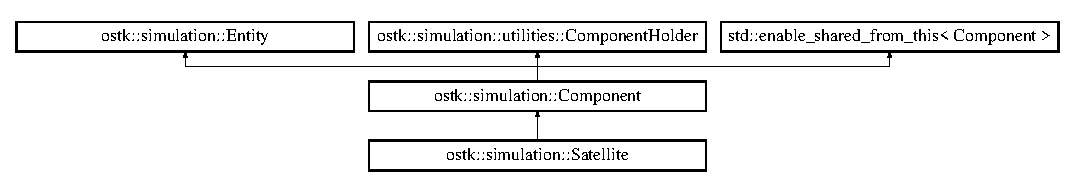
\includegraphics[height=2.066421cm]{classostk_1_1simulation_1_1_satellite}
\end{center}
\end{figure}
\doxysubsection*{Public Member Functions}
\begin{DoxyCompactItemize}
\item 
\mbox{\hyperlink{classostk_1_1simulation_1_1_satellite_aee8265886243e5c4cf71fa376fc1e984}{Satellite}} (const String \&an\+Id, const String \&a\+Name, const Array$<$ String $>$ \&a\+Tag\+Array, const Array$<$ Shared$<$ \mbox{\hyperlink{classostk_1_1simulation_1_1component_1_1_geometry}{Geometry}} $>$$>$ \&a\+Geometry\+Array, const Array$<$ Shared$<$ \mbox{\hyperlink{classostk_1_1simulation_1_1_component}{Component}} $>$$>$ \&a\+Component\+Array, const Shared$<$ const Frame $>$ \&a\+Frame\+S\+Ptr, const Shared$<$ const Profile $>$ \&a\+Profile\+S\+Ptr, const Shared$<$ const \mbox{\hyperlink{classostk_1_1simulation_1_1_simulator}{Simulator}} $>$ \&a\+Simulator\+S\+Ptr)
\item 
\mbox{\hyperlink{classostk_1_1simulation_1_1_satellite_adb01c7d30bfc51144067e5a92709c638}{Satellite}} (const \mbox{\hyperlink{classostk_1_1simulation_1_1_satellite}{Satellite}} \&a\+Satellite)
\item 
\mbox{\hyperlink{classostk_1_1simulation_1_1_satellite_af6f1e69609eca81bda731d176a0f3786}{$\sim$\+Satellite}} ()
\item 
\mbox{\hyperlink{classostk_1_1simulation_1_1_satellite}{Satellite}} $\ast$ \mbox{\hyperlink{classostk_1_1simulation_1_1_satellite_a9828fe3ec02b8f4d8b2faf8412826f00}{clone}} () const
\item 
bool \mbox{\hyperlink{classostk_1_1simulation_1_1_satellite_a124ee57d73d12788466ba203b126fc57}{is\+Defined}} () const
\item 
const Shared$<$ const Profile $>$ \mbox{\hyperlink{classostk_1_1simulation_1_1_satellite_a165c0d2da9a36a1eaeaaba55a5752cfc}{access\+Profile}} () const
\item 
void \mbox{\hyperlink{classostk_1_1simulation_1_1_satellite_ac7f5b5462deb081eb93115f0fb362acd}{print}} (std\+::ostream \&an\+Output\+Stream, bool display\+Decorators=true) const
\begin{DoxyCompactList}\small\item\em Print satellite. \end{DoxyCompactList}\end{DoxyCompactItemize}
\doxysubsection*{Static Public Member Functions}
\begin{DoxyCompactItemize}
\item 
static \mbox{\hyperlink{classostk_1_1simulation_1_1_satellite}{Satellite}} \mbox{\hyperlink{classostk_1_1simulation_1_1_satellite_a27b1931fa0cdd157ea5920060caf05fd}{Undefined}} ()
\item 
static Shared$<$ \mbox{\hyperlink{classostk_1_1simulation_1_1_satellite}{Satellite}} $>$ \mbox{\hyperlink{classostk_1_1simulation_1_1_satellite_a8984ad4a21ba686cbae3bbfbb7d5ebb3}{Configure}} (const \mbox{\hyperlink{structostk_1_1simulation_1_1_satellite_configuration}{Satellite\+Configuration}} \&a\+Satellite\+Configuration, const Shared$<$ const \mbox{\hyperlink{classostk_1_1simulation_1_1_simulator}{Simulator}} $>$ \&a\+Simulator\+S\+Ptr)
\item 
static Shared$<$ const Frame $>$ \mbox{\hyperlink{classostk_1_1simulation_1_1_satellite_a39a4b79c04d242d85cb647abd23e9e61}{Generate\+Frame}} (const String \&a\+Name, const Shared$<$ const Profile $>$ \&a\+Profile)
\end{DoxyCompactItemize}
\doxysubsection*{Friends}
\begin{DoxyCompactItemize}
\item 
std\+::ostream \& \mbox{\hyperlink{classostk_1_1simulation_1_1_satellite_a4c904b132bff149960ba9d910ebbc3dc}{operator$<$$<$}} (std\+::ostream \&an\+Output\+Stream, const \mbox{\hyperlink{classostk_1_1simulation_1_1_satellite}{Satellite}} \&a\+Satellite)
\end{DoxyCompactItemize}
\doxysubsection*{Additional Inherited Members}


\doxysubsection{Detailed Description}
\mbox{\hyperlink{classostk_1_1simulation_1_1_satellite}{Satellite}}. 

\doxysubsection{Constructor \& Destructor Documentation}
\mbox{\Hypertarget{classostk_1_1simulation_1_1_satellite_aee8265886243e5c4cf71fa376fc1e984}\label{classostk_1_1simulation_1_1_satellite_aee8265886243e5c4cf71fa376fc1e984}} 
\index{ostk::simulation::Satellite@{ostk::simulation::Satellite}!Satellite@{Satellite}}
\index{Satellite@{Satellite}!ostk::simulation::Satellite@{ostk::simulation::Satellite}}
\doxysubsubsection{\texorpdfstring{Satellite()}{Satellite()}\hspace{0.1cm}{\footnotesize\ttfamily [1/2]}}
{\footnotesize\ttfamily ostk\+::simulation\+::\+Satellite\+::\+Satellite (\begin{DoxyParamCaption}\item[{const String \&}]{an\+Id,  }\item[{const String \&}]{a\+Name,  }\item[{const Array$<$ String $>$ \&}]{a\+Tag\+Array,  }\item[{const Array$<$ Shared$<$ \mbox{\hyperlink{classostk_1_1simulation_1_1component_1_1_geometry}{Geometry}} $>$$>$ \&}]{a\+Geometry\+Array,  }\item[{const Array$<$ Shared$<$ \mbox{\hyperlink{classostk_1_1simulation_1_1_component}{Component}} $>$$>$ \&}]{a\+Component\+Array,  }\item[{const Shared$<$ const Frame $>$ \&}]{a\+Frame\+S\+Ptr,  }\item[{const Shared$<$ const Profile $>$ \&}]{a\+Profile\+S\+Ptr,  }\item[{const Shared$<$ const \mbox{\hyperlink{classostk_1_1simulation_1_1_simulator}{Simulator}} $>$ \&}]{a\+Simulator\+S\+Ptr }\end{DoxyParamCaption})}

\mbox{\Hypertarget{classostk_1_1simulation_1_1_satellite_adb01c7d30bfc51144067e5a92709c638}\label{classostk_1_1simulation_1_1_satellite_adb01c7d30bfc51144067e5a92709c638}} 
\index{ostk::simulation::Satellite@{ostk::simulation::Satellite}!Satellite@{Satellite}}
\index{Satellite@{Satellite}!ostk::simulation::Satellite@{ostk::simulation::Satellite}}
\doxysubsubsection{\texorpdfstring{Satellite()}{Satellite()}\hspace{0.1cm}{\footnotesize\ttfamily [2/2]}}
{\footnotesize\ttfamily ostk\+::simulation\+::\+Satellite\+::\+Satellite (\begin{DoxyParamCaption}\item[{const \mbox{\hyperlink{classostk_1_1simulation_1_1_satellite}{Satellite}} \&}]{a\+Satellite }\end{DoxyParamCaption})}

\mbox{\Hypertarget{classostk_1_1simulation_1_1_satellite_af6f1e69609eca81bda731d176a0f3786}\label{classostk_1_1simulation_1_1_satellite_af6f1e69609eca81bda731d176a0f3786}} 
\index{ostk::simulation::Satellite@{ostk::simulation::Satellite}!````~Satellite@{$\sim$Satellite}}
\index{````~Satellite@{$\sim$Satellite}!ostk::simulation::Satellite@{ostk::simulation::Satellite}}
\doxysubsubsection{\texorpdfstring{$\sim$Satellite()}{~Satellite()}}
{\footnotesize\ttfamily ostk\+::simulation\+::\+Satellite\+::$\sim$\+Satellite (\begin{DoxyParamCaption}{ }\end{DoxyParamCaption})}



\doxysubsection{Member Function Documentation}
\mbox{\Hypertarget{classostk_1_1simulation_1_1_satellite_a165c0d2da9a36a1eaeaaba55a5752cfc}\label{classostk_1_1simulation_1_1_satellite_a165c0d2da9a36a1eaeaaba55a5752cfc}} 
\index{ostk::simulation::Satellite@{ostk::simulation::Satellite}!accessProfile@{accessProfile}}
\index{accessProfile@{accessProfile}!ostk::simulation::Satellite@{ostk::simulation::Satellite}}
\doxysubsubsection{\texorpdfstring{accessProfile()}{accessProfile()}}
{\footnotesize\ttfamily const Shared$<$ const Profile $>$ ostk\+::simulation\+::\+Satellite\+::access\+Profile (\begin{DoxyParamCaption}{ }\end{DoxyParamCaption}) const}

\mbox{\Hypertarget{classostk_1_1simulation_1_1_satellite_a9828fe3ec02b8f4d8b2faf8412826f00}\label{classostk_1_1simulation_1_1_satellite_a9828fe3ec02b8f4d8b2faf8412826f00}} 
\index{ostk::simulation::Satellite@{ostk::simulation::Satellite}!clone@{clone}}
\index{clone@{clone}!ostk::simulation::Satellite@{ostk::simulation::Satellite}}
\doxysubsubsection{\texorpdfstring{clone()}{clone()}}
{\footnotesize\ttfamily \mbox{\hyperlink{classostk_1_1simulation_1_1_satellite}{Satellite}} $\ast$ ostk\+::simulation\+::\+Satellite\+::clone (\begin{DoxyParamCaption}{ }\end{DoxyParamCaption}) const\hspace{0.3cm}{\ttfamily [virtual]}}



Reimplemented from \mbox{\hyperlink{classostk_1_1simulation_1_1_component_a36cdd3498146b23e3ff67b95cd1c59cc}{ostk\+::simulation\+::\+Component}}.

\mbox{\Hypertarget{classostk_1_1simulation_1_1_satellite_a8984ad4a21ba686cbae3bbfbb7d5ebb3}\label{classostk_1_1simulation_1_1_satellite_a8984ad4a21ba686cbae3bbfbb7d5ebb3}} 
\index{ostk::simulation::Satellite@{ostk::simulation::Satellite}!Configure@{Configure}}
\index{Configure@{Configure}!ostk::simulation::Satellite@{ostk::simulation::Satellite}}
\doxysubsubsection{\texorpdfstring{Configure()}{Configure()}}
{\footnotesize\ttfamily Shared$<$ \mbox{\hyperlink{classostk_1_1simulation_1_1_satellite}{Satellite}} $>$ ostk\+::simulation\+::\+Satellite\+::\+Configure (\begin{DoxyParamCaption}\item[{const \mbox{\hyperlink{structostk_1_1simulation_1_1_satellite_configuration}{Satellite\+Configuration}} \&}]{a\+Satellite\+Configuration,  }\item[{const Shared$<$ const \mbox{\hyperlink{classostk_1_1simulation_1_1_simulator}{Simulator}} $>$ \&}]{a\+Simulator\+S\+Ptr }\end{DoxyParamCaption})\hspace{0.3cm}{\ttfamily [static]}}

\mbox{\Hypertarget{classostk_1_1simulation_1_1_satellite_a39a4b79c04d242d85cb647abd23e9e61}\label{classostk_1_1simulation_1_1_satellite_a39a4b79c04d242d85cb647abd23e9e61}} 
\index{ostk::simulation::Satellite@{ostk::simulation::Satellite}!GenerateFrame@{GenerateFrame}}
\index{GenerateFrame@{GenerateFrame}!ostk::simulation::Satellite@{ostk::simulation::Satellite}}
\doxysubsubsection{\texorpdfstring{GenerateFrame()}{GenerateFrame()}}
{\footnotesize\ttfamily Shared$<$ const Frame $>$ ostk\+::simulation\+::\+Satellite\+::\+Generate\+Frame (\begin{DoxyParamCaption}\item[{const String \&}]{a\+Name,  }\item[{const Shared$<$ const Profile $>$ \&}]{a\+Profile }\end{DoxyParamCaption})\hspace{0.3cm}{\ttfamily [static]}}

\mbox{\Hypertarget{classostk_1_1simulation_1_1_satellite_a124ee57d73d12788466ba203b126fc57}\label{classostk_1_1simulation_1_1_satellite_a124ee57d73d12788466ba203b126fc57}} 
\index{ostk::simulation::Satellite@{ostk::simulation::Satellite}!isDefined@{isDefined}}
\index{isDefined@{isDefined}!ostk::simulation::Satellite@{ostk::simulation::Satellite}}
\doxysubsubsection{\texorpdfstring{isDefined()}{isDefined()}}
{\footnotesize\ttfamily bool ostk\+::simulation\+::\+Satellite\+::is\+Defined (\begin{DoxyParamCaption}{ }\end{DoxyParamCaption}) const}

\mbox{\Hypertarget{classostk_1_1simulation_1_1_satellite_ac7f5b5462deb081eb93115f0fb362acd}\label{classostk_1_1simulation_1_1_satellite_ac7f5b5462deb081eb93115f0fb362acd}} 
\index{ostk::simulation::Satellite@{ostk::simulation::Satellite}!print@{print}}
\index{print@{print}!ostk::simulation::Satellite@{ostk::simulation::Satellite}}
\doxysubsubsection{\texorpdfstring{print()}{print()}}
{\footnotesize\ttfamily void ostk\+::simulation\+::\+Satellite\+::print (\begin{DoxyParamCaption}\item[{std\+::ostream \&}]{an\+Output\+Stream,  }\item[{bool}]{display\+Decorators = {\ttfamily true} }\end{DoxyParamCaption}) const\hspace{0.3cm}{\ttfamily [virtual]}}



Print satellite. 


\begin{DoxyParams}[1]{Parameters}
\mbox{\texttt{ in}}  & {\em an\+Output\+Stream} & An output stream \\
\hline
\mbox{\texttt{ in}}  & {\em (optional)} & display\+Decorators If true, display decorators \\
\hline
\end{DoxyParams}


Reimplemented from \mbox{\hyperlink{classostk_1_1simulation_1_1_component_a9c102937dd6ca5fb9e3b726cc0fd5ed6}{ostk\+::simulation\+::\+Component}}.

\mbox{\Hypertarget{classostk_1_1simulation_1_1_satellite_a27b1931fa0cdd157ea5920060caf05fd}\label{classostk_1_1simulation_1_1_satellite_a27b1931fa0cdd157ea5920060caf05fd}} 
\index{ostk::simulation::Satellite@{ostk::simulation::Satellite}!Undefined@{Undefined}}
\index{Undefined@{Undefined}!ostk::simulation::Satellite@{ostk::simulation::Satellite}}
\doxysubsubsection{\texorpdfstring{Undefined()}{Undefined()}}
{\footnotesize\ttfamily \mbox{\hyperlink{classostk_1_1simulation_1_1_satellite}{Satellite}} ostk\+::simulation\+::\+Satellite\+::\+Undefined (\begin{DoxyParamCaption}{ }\end{DoxyParamCaption})\hspace{0.3cm}{\ttfamily [static]}}



\doxysubsection{Friends And Related Function Documentation}
\mbox{\Hypertarget{classostk_1_1simulation_1_1_satellite_a4c904b132bff149960ba9d910ebbc3dc}\label{classostk_1_1simulation_1_1_satellite_a4c904b132bff149960ba9d910ebbc3dc}} 
\index{ostk::simulation::Satellite@{ostk::simulation::Satellite}!operator$<$$<$@{operator$<$$<$}}
\index{operator$<$$<$@{operator$<$$<$}!ostk::simulation::Satellite@{ostk::simulation::Satellite}}
\doxysubsubsection{\texorpdfstring{operator$<$$<$}{operator<<}}
{\footnotesize\ttfamily std\+::ostream\& operator$<$$<$ (\begin{DoxyParamCaption}\item[{std\+::ostream \&}]{an\+Output\+Stream,  }\item[{const \mbox{\hyperlink{classostk_1_1simulation_1_1_satellite}{Satellite}} \&}]{a\+Satellite }\end{DoxyParamCaption})\hspace{0.3cm}{\ttfamily [friend]}}



The documentation for this class was generated from the following files\+:\begin{DoxyCompactItemize}
\item 
include/\+Open\+Space\+Toolkit/\+Simulation/\mbox{\hyperlink{_satellite_8hpp}{Satellite.\+hpp}}\item 
src/\+Open\+Space\+Toolkit/\+Simulation/\mbox{\hyperlink{_satellite_8cpp}{Satellite.\+cpp}}\end{DoxyCompactItemize}

\hypertarget{structostk_1_1simulation_1_1_satellite_configuration}{}\section{ostk\+:\+:simulation\+:\+:Satellite\+Configuration Struct Reference}
\label{structostk_1_1simulation_1_1_satellite_configuration}\index{ostk\+::simulation\+::\+Satellite\+Configuration@{ostk\+::simulation\+::\+Satellite\+Configuration}}


{\ttfamily \#include $<$Satellite.\+hpp$>$}

\subsection*{Public Attributes}
\begin{DoxyCompactItemize}
\item 
const String \hyperlink{structostk_1_1simulation_1_1_satellite_configuration_a908266db30927a86a162c7c8a73bdbe1}{id}
\item 
const String \hyperlink{structostk_1_1simulation_1_1_satellite_configuration_a5591546d238904643014391632e95073}{name}
\item 
const Profile \hyperlink{structostk_1_1simulation_1_1_satellite_configuration_ab2afb3f9823e69021f909495fb74ca3f}{profile}
\item 
const Array$<$ \hyperlink{structostk_1_1simulation_1_1_component_configuration}{Component\+Configuration} $>$ \hyperlink{structostk_1_1simulation_1_1_satellite_configuration_a44d10b5d983f71491e0751a0c1ac5f80}{components} = \hyperlink{_satellite_8hpp_a4efe76b184101f122bb1be222cb65afc}{D\+E\+F\+A\+U\+L\+T\+\_\+\+C\+O\+M\+P\+O\+N\+E\+N\+TS}
\item 
const Array$<$ String $>$ \hyperlink{structostk_1_1simulation_1_1_satellite_configuration_a6db145a39cbb82053013b7ee92dcc326}{tags} = \hyperlink{_satellite_8hpp_a7cabb8538f234177d4f95e681045bf94}{D\+E\+F\+A\+U\+L\+T\+\_\+\+T\+A\+GS}
\item 
const Array$<$ \hyperlink{structostk_1_1simulation_1_1component_1_1_geometry_configuration}{Geometry\+Configuration} $>$ \hyperlink{structostk_1_1simulation_1_1_satellite_configuration_aea05ae6081923cf5c9502bd176b756b9}{geometries} = \hyperlink{_satellite_8hpp_a4a68d11996a67b508045cdc894fac4ba}{D\+E\+F\+A\+U\+L\+T\+\_\+\+G\+E\+O\+M\+E\+T\+R\+I\+ES}
\end{DoxyCompactItemize}


\subsection{Member Data Documentation}
\mbox{\Hypertarget{structostk_1_1simulation_1_1_satellite_configuration_a44d10b5d983f71491e0751a0c1ac5f80}\label{structostk_1_1simulation_1_1_satellite_configuration_a44d10b5d983f71491e0751a0c1ac5f80}} 
\index{ostk\+::simulation\+::\+Satellite\+Configuration@{ostk\+::simulation\+::\+Satellite\+Configuration}!components@{components}}
\index{components@{components}!ostk\+::simulation\+::\+Satellite\+Configuration@{ostk\+::simulation\+::\+Satellite\+Configuration}}
\subsubsection{\texorpdfstring{components}{components}}
{\footnotesize\ttfamily const Array$<$\hyperlink{structostk_1_1simulation_1_1_component_configuration}{Component\+Configuration}$>$ ostk\+::simulation\+::\+Satellite\+Configuration\+::components = \hyperlink{_satellite_8hpp_a4efe76b184101f122bb1be222cb65afc}{D\+E\+F\+A\+U\+L\+T\+\_\+\+C\+O\+M\+P\+O\+N\+E\+N\+TS}}

\mbox{\Hypertarget{structostk_1_1simulation_1_1_satellite_configuration_aea05ae6081923cf5c9502bd176b756b9}\label{structostk_1_1simulation_1_1_satellite_configuration_aea05ae6081923cf5c9502bd176b756b9}} 
\index{ostk\+::simulation\+::\+Satellite\+Configuration@{ostk\+::simulation\+::\+Satellite\+Configuration}!geometries@{geometries}}
\index{geometries@{geometries}!ostk\+::simulation\+::\+Satellite\+Configuration@{ostk\+::simulation\+::\+Satellite\+Configuration}}
\subsubsection{\texorpdfstring{geometries}{geometries}}
{\footnotesize\ttfamily const Array$<$\hyperlink{structostk_1_1simulation_1_1component_1_1_geometry_configuration}{Geometry\+Configuration}$>$ ostk\+::simulation\+::\+Satellite\+Configuration\+::geometries = \hyperlink{_satellite_8hpp_a4a68d11996a67b508045cdc894fac4ba}{D\+E\+F\+A\+U\+L\+T\+\_\+\+G\+E\+O\+M\+E\+T\+R\+I\+ES}}

\mbox{\Hypertarget{structostk_1_1simulation_1_1_satellite_configuration_a908266db30927a86a162c7c8a73bdbe1}\label{structostk_1_1simulation_1_1_satellite_configuration_a908266db30927a86a162c7c8a73bdbe1}} 
\index{ostk\+::simulation\+::\+Satellite\+Configuration@{ostk\+::simulation\+::\+Satellite\+Configuration}!id@{id}}
\index{id@{id}!ostk\+::simulation\+::\+Satellite\+Configuration@{ostk\+::simulation\+::\+Satellite\+Configuration}}
\subsubsection{\texorpdfstring{id}{id}}
{\footnotesize\ttfamily const String ostk\+::simulation\+::\+Satellite\+Configuration\+::id}

\mbox{\Hypertarget{structostk_1_1simulation_1_1_satellite_configuration_a5591546d238904643014391632e95073}\label{structostk_1_1simulation_1_1_satellite_configuration_a5591546d238904643014391632e95073}} 
\index{ostk\+::simulation\+::\+Satellite\+Configuration@{ostk\+::simulation\+::\+Satellite\+Configuration}!name@{name}}
\index{name@{name}!ostk\+::simulation\+::\+Satellite\+Configuration@{ostk\+::simulation\+::\+Satellite\+Configuration}}
\subsubsection{\texorpdfstring{name}{name}}
{\footnotesize\ttfamily const String ostk\+::simulation\+::\+Satellite\+Configuration\+::name}

\mbox{\Hypertarget{structostk_1_1simulation_1_1_satellite_configuration_ab2afb3f9823e69021f909495fb74ca3f}\label{structostk_1_1simulation_1_1_satellite_configuration_ab2afb3f9823e69021f909495fb74ca3f}} 
\index{ostk\+::simulation\+::\+Satellite\+Configuration@{ostk\+::simulation\+::\+Satellite\+Configuration}!profile@{profile}}
\index{profile@{profile}!ostk\+::simulation\+::\+Satellite\+Configuration@{ostk\+::simulation\+::\+Satellite\+Configuration}}
\subsubsection{\texorpdfstring{profile}{profile}}
{\footnotesize\ttfamily const Profile ostk\+::simulation\+::\+Satellite\+Configuration\+::profile}

\mbox{\Hypertarget{structostk_1_1simulation_1_1_satellite_configuration_a6db145a39cbb82053013b7ee92dcc326}\label{structostk_1_1simulation_1_1_satellite_configuration_a6db145a39cbb82053013b7ee92dcc326}} 
\index{ostk\+::simulation\+::\+Satellite\+Configuration@{ostk\+::simulation\+::\+Satellite\+Configuration}!tags@{tags}}
\index{tags@{tags}!ostk\+::simulation\+::\+Satellite\+Configuration@{ostk\+::simulation\+::\+Satellite\+Configuration}}
\subsubsection{\texorpdfstring{tags}{tags}}
{\footnotesize\ttfamily const Array$<$String$>$ ostk\+::simulation\+::\+Satellite\+Configuration\+::tags = \hyperlink{_satellite_8hpp_a7cabb8538f234177d4f95e681045bf94}{D\+E\+F\+A\+U\+L\+T\+\_\+\+T\+A\+GS}}



The documentation for this struct was generated from the following file\+:\begin{DoxyCompactItemize}
\item 
include/\+Open\+Space\+Toolkit/\+Simulation/\hyperlink{_satellite_8hpp}{Satellite.\+hpp}\end{DoxyCompactItemize}

\hypertarget{classostk_1_1simulation_1_1_simulator}{}\section{ostk\+:\+:simulation\+:\+:Simulator Class Reference}
\label{classostk_1_1simulation_1_1_simulator}\index{ostk\+::simulation\+::\+Simulator@{ostk\+::simulation\+::\+Simulator}}


\hyperlink{classostk_1_1simulation_1_1_simulator}{Simulator}.  




{\ttfamily \#include $<$Simulator.\+hpp$>$}

\subsection*{Public Member Functions}
\begin{DoxyCompactItemize}
\item 
\hyperlink{classostk_1_1simulation_1_1_simulator_a6c69bdb82f84e62d0e006755d501e05a}{Simulator} (const Environment \&an\+Environment, const Array$<$ Shared$<$ \hyperlink{classostk_1_1simulation_1_1_satellite}{Satellite} $>$$>$ \&a\+Satellite\+Array)
\item 
bool \hyperlink{classostk_1_1simulation_1_1_simulator_a666148ccdc39474edbe83e7ffc65bac1}{is\+Defined} () const
\item 
bool \hyperlink{classostk_1_1simulation_1_1_simulator_a055842428d08ac13305da1b3ad339568}{has\+Satellite\+With\+Name} (const String \&a\+Satellite\+Name) const
\item 
const Environment \& \hyperlink{classostk_1_1simulation_1_1_simulator_aa1c20421b7a2ad00954fea7bdfbd4edd}{access\+Environment} () const
\item 
const \hyperlink{classostk_1_1simulation_1_1_satellite}{Satellite} \& \hyperlink{classostk_1_1simulation_1_1_simulator_ada54ce66cb47bb512f245f4ac1b33f95}{access\+Satellite\+With\+Name} (const String \&a\+Satellite\+Name) const
\item 
Instant \hyperlink{classostk_1_1simulation_1_1_simulator_a64483af631b1f905850bb8b366f6fb0a}{get\+Instant} () const
\item 
void \hyperlink{classostk_1_1simulation_1_1_simulator_a820c217ea08c035aa3b171112998b334}{print} (std\+::ostream \&an\+Output\+Stream, bool display\+Decorators=true) const
\begin{DoxyCompactList}\small\item\em Print simulator. \end{DoxyCompactList}\item 
void \hyperlink{classostk_1_1simulation_1_1_simulator_ab5fb0cb4864bbbbb35b3ab65d76d0a84}{set\+Instant} (const Instant \&an\+Instant)
\item 
void \hyperlink{classostk_1_1simulation_1_1_simulator_acb6015e28195acde22acc04ff2e8b8a8}{step\+Forward} (const Duration \&a\+Duration)
\item 
void \hyperlink{classostk_1_1simulation_1_1_simulator_a03e47de54e6db4942b77d24c46dcc940}{add\+Satellite} (const Shared$<$ \hyperlink{classostk_1_1simulation_1_1_satellite}{Satellite} $>$ \&a\+Satellite\+S\+Ptr)
\end{DoxyCompactItemize}
\subsection*{Static Public Member Functions}
\begin{DoxyCompactItemize}
\item 
static \hyperlink{classostk_1_1simulation_1_1_simulator}{Simulator} \hyperlink{classostk_1_1simulation_1_1_simulator_a99876309ee0abbb7fb47b232bb28e6db}{Undefined} ()
\item 
static Shared$<$ \hyperlink{classostk_1_1simulation_1_1_simulator}{Simulator} $>$ \hyperlink{classostk_1_1simulation_1_1_simulator_ad95b067abdc0a5ddf348897161af46f1}{Configure} (const \hyperlink{structostk_1_1simulation_1_1_simulator_configuration}{Simulator\+Configuration} \&a\+Simulator\+Configuration)
\end{DoxyCompactItemize}
\subsection*{Friends}
\begin{DoxyCompactItemize}
\item 
std\+::ostream \& \hyperlink{classostk_1_1simulation_1_1_simulator_a69c38d700ebaa96e61bccca4bdbe717d}{operator$<$$<$} (std\+::ostream \&an\+Output\+Stream, const \hyperlink{classostk_1_1simulation_1_1_simulator}{Simulator} \&a\+Simulator)
\end{DoxyCompactItemize}


\subsection{Detailed Description}
\hyperlink{classostk_1_1simulation_1_1_simulator}{Simulator}. 

\subsection{Constructor \& Destructor Documentation}
\mbox{\Hypertarget{classostk_1_1simulation_1_1_simulator_a6c69bdb82f84e62d0e006755d501e05a}\label{classostk_1_1simulation_1_1_simulator_a6c69bdb82f84e62d0e006755d501e05a}} 
\index{ostk\+::simulation\+::\+Simulator@{ostk\+::simulation\+::\+Simulator}!Simulator@{Simulator}}
\index{Simulator@{Simulator}!ostk\+::simulation\+::\+Simulator@{ostk\+::simulation\+::\+Simulator}}
\subsubsection{\texorpdfstring{Simulator()}{Simulator()}}
{\footnotesize\ttfamily ostk\+::simulation\+::\+Simulator\+::\+Simulator (\begin{DoxyParamCaption}\item[{const Environment \&}]{an\+Environment,  }\item[{const Array$<$ Shared$<$ \hyperlink{classostk_1_1simulation_1_1_satellite}{Satellite} $>$$>$ \&}]{a\+Satellite\+Array }\end{DoxyParamCaption})}



\subsection{Member Function Documentation}
\mbox{\Hypertarget{classostk_1_1simulation_1_1_simulator_aa1c20421b7a2ad00954fea7bdfbd4edd}\label{classostk_1_1simulation_1_1_simulator_aa1c20421b7a2ad00954fea7bdfbd4edd}} 
\index{ostk\+::simulation\+::\+Simulator@{ostk\+::simulation\+::\+Simulator}!access\+Environment@{access\+Environment}}
\index{access\+Environment@{access\+Environment}!ostk\+::simulation\+::\+Simulator@{ostk\+::simulation\+::\+Simulator}}
\subsubsection{\texorpdfstring{access\+Environment()}{accessEnvironment()}}
{\footnotesize\ttfamily const Environment \& ostk\+::simulation\+::\+Simulator\+::access\+Environment (\begin{DoxyParamCaption}{ }\end{DoxyParamCaption}) const}

\mbox{\Hypertarget{classostk_1_1simulation_1_1_simulator_ada54ce66cb47bb512f245f4ac1b33f95}\label{classostk_1_1simulation_1_1_simulator_ada54ce66cb47bb512f245f4ac1b33f95}} 
\index{ostk\+::simulation\+::\+Simulator@{ostk\+::simulation\+::\+Simulator}!access\+Satellite\+With\+Name@{access\+Satellite\+With\+Name}}
\index{access\+Satellite\+With\+Name@{access\+Satellite\+With\+Name}!ostk\+::simulation\+::\+Simulator@{ostk\+::simulation\+::\+Simulator}}
\subsubsection{\texorpdfstring{access\+Satellite\+With\+Name()}{accessSatelliteWithName()}}
{\footnotesize\ttfamily const \hyperlink{classostk_1_1simulation_1_1_satellite}{Satellite} \& ostk\+::simulation\+::\+Simulator\+::access\+Satellite\+With\+Name (\begin{DoxyParamCaption}\item[{const String \&}]{a\+Satellite\+Name }\end{DoxyParamCaption}) const}

\mbox{\Hypertarget{classostk_1_1simulation_1_1_simulator_a03e47de54e6db4942b77d24c46dcc940}\label{classostk_1_1simulation_1_1_simulator_a03e47de54e6db4942b77d24c46dcc940}} 
\index{ostk\+::simulation\+::\+Simulator@{ostk\+::simulation\+::\+Simulator}!add\+Satellite@{add\+Satellite}}
\index{add\+Satellite@{add\+Satellite}!ostk\+::simulation\+::\+Simulator@{ostk\+::simulation\+::\+Simulator}}
\subsubsection{\texorpdfstring{add\+Satellite()}{addSatellite()}}
{\footnotesize\ttfamily void ostk\+::simulation\+::\+Simulator\+::add\+Satellite (\begin{DoxyParamCaption}\item[{const Shared$<$ \hyperlink{classostk_1_1simulation_1_1_satellite}{Satellite} $>$ \&}]{a\+Satellite\+S\+Ptr }\end{DoxyParamCaption})}

\mbox{\Hypertarget{classostk_1_1simulation_1_1_simulator_ad95b067abdc0a5ddf348897161af46f1}\label{classostk_1_1simulation_1_1_simulator_ad95b067abdc0a5ddf348897161af46f1}} 
\index{ostk\+::simulation\+::\+Simulator@{ostk\+::simulation\+::\+Simulator}!Configure@{Configure}}
\index{Configure@{Configure}!ostk\+::simulation\+::\+Simulator@{ostk\+::simulation\+::\+Simulator}}
\subsubsection{\texorpdfstring{Configure()}{Configure()}}
{\footnotesize\ttfamily Shared$<$ \hyperlink{classostk_1_1simulation_1_1_simulator}{Simulator} $>$ ostk\+::simulation\+::\+Simulator\+::\+Configure (\begin{DoxyParamCaption}\item[{const \hyperlink{structostk_1_1simulation_1_1_simulator_configuration}{Simulator\+Configuration} \&}]{a\+Simulator\+Configuration }\end{DoxyParamCaption})\hspace{0.3cm}{\ttfamily [static]}}

\mbox{\Hypertarget{classostk_1_1simulation_1_1_simulator_a64483af631b1f905850bb8b366f6fb0a}\label{classostk_1_1simulation_1_1_simulator_a64483af631b1f905850bb8b366f6fb0a}} 
\index{ostk\+::simulation\+::\+Simulator@{ostk\+::simulation\+::\+Simulator}!get\+Instant@{get\+Instant}}
\index{get\+Instant@{get\+Instant}!ostk\+::simulation\+::\+Simulator@{ostk\+::simulation\+::\+Simulator}}
\subsubsection{\texorpdfstring{get\+Instant()}{getInstant()}}
{\footnotesize\ttfamily Instant ostk\+::simulation\+::\+Simulator\+::get\+Instant (\begin{DoxyParamCaption}{ }\end{DoxyParamCaption}) const}

\mbox{\Hypertarget{classostk_1_1simulation_1_1_simulator_a055842428d08ac13305da1b3ad339568}\label{classostk_1_1simulation_1_1_simulator_a055842428d08ac13305da1b3ad339568}} 
\index{ostk\+::simulation\+::\+Simulator@{ostk\+::simulation\+::\+Simulator}!has\+Satellite\+With\+Name@{has\+Satellite\+With\+Name}}
\index{has\+Satellite\+With\+Name@{has\+Satellite\+With\+Name}!ostk\+::simulation\+::\+Simulator@{ostk\+::simulation\+::\+Simulator}}
\subsubsection{\texorpdfstring{has\+Satellite\+With\+Name()}{hasSatelliteWithName()}}
{\footnotesize\ttfamily bool ostk\+::simulation\+::\+Simulator\+::has\+Satellite\+With\+Name (\begin{DoxyParamCaption}\item[{const String \&}]{a\+Satellite\+Name }\end{DoxyParamCaption}) const}

\mbox{\Hypertarget{classostk_1_1simulation_1_1_simulator_a666148ccdc39474edbe83e7ffc65bac1}\label{classostk_1_1simulation_1_1_simulator_a666148ccdc39474edbe83e7ffc65bac1}} 
\index{ostk\+::simulation\+::\+Simulator@{ostk\+::simulation\+::\+Simulator}!is\+Defined@{is\+Defined}}
\index{is\+Defined@{is\+Defined}!ostk\+::simulation\+::\+Simulator@{ostk\+::simulation\+::\+Simulator}}
\subsubsection{\texorpdfstring{is\+Defined()}{isDefined()}}
{\footnotesize\ttfamily bool ostk\+::simulation\+::\+Simulator\+::is\+Defined (\begin{DoxyParamCaption}{ }\end{DoxyParamCaption}) const}

\mbox{\Hypertarget{classostk_1_1simulation_1_1_simulator_a820c217ea08c035aa3b171112998b334}\label{classostk_1_1simulation_1_1_simulator_a820c217ea08c035aa3b171112998b334}} 
\index{ostk\+::simulation\+::\+Simulator@{ostk\+::simulation\+::\+Simulator}!print@{print}}
\index{print@{print}!ostk\+::simulation\+::\+Simulator@{ostk\+::simulation\+::\+Simulator}}
\subsubsection{\texorpdfstring{print()}{print()}}
{\footnotesize\ttfamily void ostk\+::simulation\+::\+Simulator\+::print (\begin{DoxyParamCaption}\item[{std\+::ostream \&}]{an\+Output\+Stream,  }\item[{bool}]{display\+Decorators = {\ttfamily true} }\end{DoxyParamCaption}) const}



Print simulator. 


\begin{DoxyParams}[1]{Parameters}
\mbox{\tt in}  & {\em an\+Output\+Stream} & An output stream \\
\hline
\mbox{\tt in}  & {\em (optional)} & display\+Decorators If true, display decorators \\
\hline
\end{DoxyParams}
\mbox{\Hypertarget{classostk_1_1simulation_1_1_simulator_ab5fb0cb4864bbbbb35b3ab65d76d0a84}\label{classostk_1_1simulation_1_1_simulator_ab5fb0cb4864bbbbb35b3ab65d76d0a84}} 
\index{ostk\+::simulation\+::\+Simulator@{ostk\+::simulation\+::\+Simulator}!set\+Instant@{set\+Instant}}
\index{set\+Instant@{set\+Instant}!ostk\+::simulation\+::\+Simulator@{ostk\+::simulation\+::\+Simulator}}
\subsubsection{\texorpdfstring{set\+Instant()}{setInstant()}}
{\footnotesize\ttfamily void ostk\+::simulation\+::\+Simulator\+::set\+Instant (\begin{DoxyParamCaption}\item[{const Instant \&}]{an\+Instant }\end{DoxyParamCaption})}

\mbox{\Hypertarget{classostk_1_1simulation_1_1_simulator_acb6015e28195acde22acc04ff2e8b8a8}\label{classostk_1_1simulation_1_1_simulator_acb6015e28195acde22acc04ff2e8b8a8}} 
\index{ostk\+::simulation\+::\+Simulator@{ostk\+::simulation\+::\+Simulator}!step\+Forward@{step\+Forward}}
\index{step\+Forward@{step\+Forward}!ostk\+::simulation\+::\+Simulator@{ostk\+::simulation\+::\+Simulator}}
\subsubsection{\texorpdfstring{step\+Forward()}{stepForward()}}
{\footnotesize\ttfamily void ostk\+::simulation\+::\+Simulator\+::step\+Forward (\begin{DoxyParamCaption}\item[{const Duration \&}]{a\+Duration }\end{DoxyParamCaption})}

\mbox{\Hypertarget{classostk_1_1simulation_1_1_simulator_a99876309ee0abbb7fb47b232bb28e6db}\label{classostk_1_1simulation_1_1_simulator_a99876309ee0abbb7fb47b232bb28e6db}} 
\index{ostk\+::simulation\+::\+Simulator@{ostk\+::simulation\+::\+Simulator}!Undefined@{Undefined}}
\index{Undefined@{Undefined}!ostk\+::simulation\+::\+Simulator@{ostk\+::simulation\+::\+Simulator}}
\subsubsection{\texorpdfstring{Undefined()}{Undefined()}}
{\footnotesize\ttfamily \hyperlink{classostk_1_1simulation_1_1_simulator}{Simulator} ostk\+::simulation\+::\+Simulator\+::\+Undefined (\begin{DoxyParamCaption}{ }\end{DoxyParamCaption})\hspace{0.3cm}{\ttfamily [static]}}



\subsection{Friends And Related Function Documentation}
\mbox{\Hypertarget{classostk_1_1simulation_1_1_simulator_a69c38d700ebaa96e61bccca4bdbe717d}\label{classostk_1_1simulation_1_1_simulator_a69c38d700ebaa96e61bccca4bdbe717d}} 
\index{ostk\+::simulation\+::\+Simulator@{ostk\+::simulation\+::\+Simulator}!operator$<$$<$@{operator$<$$<$}}
\index{operator$<$$<$@{operator$<$$<$}!ostk\+::simulation\+::\+Simulator@{ostk\+::simulation\+::\+Simulator}}
\subsubsection{\texorpdfstring{operator$<$$<$}{operator<<}}
{\footnotesize\ttfamily std\+::ostream\& operator$<$$<$ (\begin{DoxyParamCaption}\item[{std\+::ostream \&}]{an\+Output\+Stream,  }\item[{const \hyperlink{classostk_1_1simulation_1_1_simulator}{Simulator} \&}]{a\+Simulator }\end{DoxyParamCaption})\hspace{0.3cm}{\ttfamily [friend]}}



The documentation for this class was generated from the following files\+:\begin{DoxyCompactItemize}
\item 
include/\+Open\+Space\+Toolkit/\+Simulation/\hyperlink{_simulator_8hpp}{Simulator.\+hpp}\item 
src/\+Open\+Space\+Toolkit/\+Simulation/\hyperlink{_simulator_8cpp}{Simulator.\+cpp}\end{DoxyCompactItemize}

\hypertarget{structostk_1_1simulation_1_1_simulator_configuration}{}\section{ostk\+:\+:simulation\+:\+:Simulator\+Configuration Struct Reference}
\label{structostk_1_1simulation_1_1_simulator_configuration}\index{ostk\+::simulation\+::\+Simulator\+Configuration@{ostk\+::simulation\+::\+Simulator\+Configuration}}


{\ttfamily \#include $<$Simulator.\+hpp$>$}

\subsection*{Public Attributes}
\begin{DoxyCompactItemize}
\item 
const Environment \hyperlink{structostk_1_1simulation_1_1_simulator_configuration_a002747f47ff422d4be5745eeb476e8ea}{environment}
\item 
const Array$<$ \hyperlink{structostk_1_1simulation_1_1_satellite_configuration}{Satellite\+Configuration} $>$ \hyperlink{structostk_1_1simulation_1_1_simulator_configuration_aa42414403bb4d50e000ed4a78bac78b5}{satellites} = \hyperlink{_simulator_8hpp_a233d40e3dd62e2ffb9f35a635f34fd36}{D\+E\+F\+A\+U\+L\+T\+\_\+\+S\+A\+T\+E\+L\+L\+I\+T\+ES}
\end{DoxyCompactItemize}


\subsection{Member Data Documentation}
\mbox{\Hypertarget{structostk_1_1simulation_1_1_simulator_configuration_a002747f47ff422d4be5745eeb476e8ea}\label{structostk_1_1simulation_1_1_simulator_configuration_a002747f47ff422d4be5745eeb476e8ea}} 
\index{ostk\+::simulation\+::\+Simulator\+Configuration@{ostk\+::simulation\+::\+Simulator\+Configuration}!environment@{environment}}
\index{environment@{environment}!ostk\+::simulation\+::\+Simulator\+Configuration@{ostk\+::simulation\+::\+Simulator\+Configuration}}
\subsubsection{\texorpdfstring{environment}{environment}}
{\footnotesize\ttfamily const Environment ostk\+::simulation\+::\+Simulator\+Configuration\+::environment}

\mbox{\Hypertarget{structostk_1_1simulation_1_1_simulator_configuration_aa42414403bb4d50e000ed4a78bac78b5}\label{structostk_1_1simulation_1_1_simulator_configuration_aa42414403bb4d50e000ed4a78bac78b5}} 
\index{ostk\+::simulation\+::\+Simulator\+Configuration@{ostk\+::simulation\+::\+Simulator\+Configuration}!satellites@{satellites}}
\index{satellites@{satellites}!ostk\+::simulation\+::\+Simulator\+Configuration@{ostk\+::simulation\+::\+Simulator\+Configuration}}
\subsubsection{\texorpdfstring{satellites}{satellites}}
{\footnotesize\ttfamily const Array$<$\hyperlink{structostk_1_1simulation_1_1_satellite_configuration}{Satellite\+Configuration}$>$ ostk\+::simulation\+::\+Simulator\+Configuration\+::satellites = \hyperlink{_simulator_8hpp_a233d40e3dd62e2ffb9f35a635f34fd36}{D\+E\+F\+A\+U\+L\+T\+\_\+\+S\+A\+T\+E\+L\+L\+I\+T\+ES}}



The documentation for this struct was generated from the following file\+:\begin{DoxyCompactItemize}
\item 
include/\+Open\+Space\+Toolkit/\+Simulation/\hyperlink{_simulator_8hpp}{Simulator.\+hpp}\end{DoxyCompactItemize}

\hypertarget{classostk_1_1simulation_1_1component_1_1_state}{}\section{ostk\+:\+:simulation\+:\+:component\+:\+:State Class Reference}
\label{classostk_1_1simulation_1_1component_1_1_state}\index{ostk\+::simulation\+::component\+::\+State@{ostk\+::simulation\+::component\+::\+State}}


\hyperlink{classostk_1_1simulation_1_1_component}{Component} state.  




{\ttfamily \#include $<$State.\+hpp$>$}

\subsection*{Public Types}
\begin{DoxyCompactItemize}
\item 
enum \hyperlink{classostk_1_1simulation_1_1component_1_1_state_adb8b51feaa29b0ebd5fc7977fada7e58}{Status} \{ \newline
\hyperlink{classostk_1_1simulation_1_1component_1_1_state_adb8b51feaa29b0ebd5fc7977fada7e58aec0fc0100c4fc1ce4eea230c3dc10360}{Status\+::\+Undefined}, 
\hyperlink{classostk_1_1simulation_1_1component_1_1_state_adb8b51feaa29b0ebd5fc7977fada7e58ab9f5c797ebbf55adccdd8539a65a0241}{Status\+::\+Disabled}, 
\hyperlink{classostk_1_1simulation_1_1component_1_1_state_adb8b51feaa29b0ebd5fc7977fada7e58ae599161956d626eda4cb0a5ffb85271c}{Status\+::\+Idle}, 
\hyperlink{classostk_1_1simulation_1_1component_1_1_state_adb8b51feaa29b0ebd5fc7977fada7e58ad8a942ef2b04672adfafef0ad817a407}{Status\+::\+Busy}, 
\newline
\hyperlink{classostk_1_1simulation_1_1component_1_1_state_adb8b51feaa29b0ebd5fc7977fada7e58a902b0d55fddef6f8d651fe1035b7d4bd}{Status\+::\+Error}
 \}
\end{DoxyCompactItemize}
\subsection*{Public Member Functions}
\begin{DoxyCompactItemize}
\item 
\hyperlink{classostk_1_1simulation_1_1component_1_1_state_aef1526b3513a2165970420e7ac8b6dae}{State} (const \hyperlink{classostk_1_1simulation_1_1component_1_1_state_adb8b51feaa29b0ebd5fc7977fada7e58}{State\+::\+Status} \&a\+Status=\hyperlink{_state_8hpp_a188ce67e515b427589d4c363d1132018}{D\+E\+F\+A\+U\+L\+T\+\_\+\+S\+T\+A\+T\+US}, const bool \&is\+Verbose=\hyperlink{_state_8hpp_a4ad8faebfc1723fec1090b84ec0f680e}{D\+E\+F\+A\+U\+L\+T\+\_\+\+V\+E\+R\+B\+O\+SE})
\item 
\hyperlink{classostk_1_1simulation_1_1component_1_1_state_a36adbe9bccb78bec881e2c3f267724ed}{State} (const \hyperlink{classostk_1_1simulation_1_1component_1_1_state}{State} \&a\+State)
\item 
virtual \hyperlink{classostk_1_1simulation_1_1component_1_1_state_a57c4cf4d8c50c2482402e3740483c29e}{$\sim$\+State} ()
\item 
virtual \hyperlink{classostk_1_1simulation_1_1component_1_1_state}{State} $\ast$ \hyperlink{classostk_1_1simulation_1_1component_1_1_state_a32e9b1349918070f114cb38e61828897}{clone} () const
\item 
\hyperlink{classostk_1_1simulation_1_1component_1_1_state}{State} \& \hyperlink{classostk_1_1simulation_1_1component_1_1_state_ac8aaea99357f670afab3c087de08446f}{operator=} (const \hyperlink{classostk_1_1simulation_1_1component_1_1_state}{State} \&a\+State)
\item 
bool \hyperlink{classostk_1_1simulation_1_1component_1_1_state_ad4440388904bac640dc57ffbc5b77019}{operator==} (const \hyperlink{classostk_1_1simulation_1_1component_1_1_state}{State} \&a\+State) const
\begin{DoxyCompactList}\small\item\em Equal to operator. \end{DoxyCompactList}\item 
bool \hyperlink{classostk_1_1simulation_1_1component_1_1_state_abfb0349ee570125276b52aa2c3b1156d}{is\+Defined} () const
\item 
\hyperlink{classostk_1_1simulation_1_1component_1_1_state_adb8b51feaa29b0ebd5fc7977fada7e58}{State\+::\+Status} \hyperlink{classostk_1_1simulation_1_1component_1_1_state_a5ff60e1d912483effdb53b2b5c555cf9}{get\+Status} () const
\end{DoxyCompactItemize}
\subsection*{Static Public Member Functions}
\begin{DoxyCompactItemize}
\item 
static \hyperlink{classostk_1_1simulation_1_1component_1_1_state}{State} \hyperlink{classostk_1_1simulation_1_1component_1_1_state_a21a79240817592992c4791699b2d623f}{Undefined} ()
\end{DoxyCompactItemize}


\subsection{Detailed Description}
\hyperlink{classostk_1_1simulation_1_1_component}{Component} state. 

\subsection{Member Enumeration Documentation}
\mbox{\Hypertarget{classostk_1_1simulation_1_1component_1_1_state_adb8b51feaa29b0ebd5fc7977fada7e58}\label{classostk_1_1simulation_1_1component_1_1_state_adb8b51feaa29b0ebd5fc7977fada7e58}} 
\index{ostk\+::simulation\+::component\+::\+State@{ostk\+::simulation\+::component\+::\+State}!Status@{Status}}
\index{Status@{Status}!ostk\+::simulation\+::component\+::\+State@{ostk\+::simulation\+::component\+::\+State}}
\subsubsection{\texorpdfstring{Status}{Status}}
{\footnotesize\ttfamily enum \hyperlink{classostk_1_1simulation_1_1component_1_1_state_adb8b51feaa29b0ebd5fc7977fada7e58}{ostk\+::simulation\+::component\+::\+State\+::\+Status}\hspace{0.3cm}{\ttfamily [strong]}}

\begin{DoxyEnumFields}{Enumerator}
\raisebox{\heightof{T}}[0pt][0pt]{\index{Undefined@{Undefined}!ostk\+::simulation\+::component\+::\+State@{ostk\+::simulation\+::component\+::\+State}}\index{ostk\+::simulation\+::component\+::\+State@{ostk\+::simulation\+::component\+::\+State}!Undefined@{Undefined}}}\mbox{\Hypertarget{classostk_1_1simulation_1_1component_1_1_state_adb8b51feaa29b0ebd5fc7977fada7e58aec0fc0100c4fc1ce4eea230c3dc10360}\label{classostk_1_1simulation_1_1component_1_1_state_adb8b51feaa29b0ebd5fc7977fada7e58aec0fc0100c4fc1ce4eea230c3dc10360}} 
Undefined&\\
\hline

\raisebox{\heightof{T}}[0pt][0pt]{\index{Disabled@{Disabled}!ostk\+::simulation\+::component\+::\+State@{ostk\+::simulation\+::component\+::\+State}}\index{ostk\+::simulation\+::component\+::\+State@{ostk\+::simulation\+::component\+::\+State}!Disabled@{Disabled}}}\mbox{\Hypertarget{classostk_1_1simulation_1_1component_1_1_state_adb8b51feaa29b0ebd5fc7977fada7e58ab9f5c797ebbf55adccdd8539a65a0241}\label{classostk_1_1simulation_1_1component_1_1_state_adb8b51feaa29b0ebd5fc7977fada7e58ab9f5c797ebbf55adccdd8539a65a0241}} 
Disabled&\\
\hline

\raisebox{\heightof{T}}[0pt][0pt]{\index{Idle@{Idle}!ostk\+::simulation\+::component\+::\+State@{ostk\+::simulation\+::component\+::\+State}}\index{ostk\+::simulation\+::component\+::\+State@{ostk\+::simulation\+::component\+::\+State}!Idle@{Idle}}}\mbox{\Hypertarget{classostk_1_1simulation_1_1component_1_1_state_adb8b51feaa29b0ebd5fc7977fada7e58ae599161956d626eda4cb0a5ffb85271c}\label{classostk_1_1simulation_1_1component_1_1_state_adb8b51feaa29b0ebd5fc7977fada7e58ae599161956d626eda4cb0a5ffb85271c}} 
Idle&\\
\hline

\raisebox{\heightof{T}}[0pt][0pt]{\index{Busy@{Busy}!ostk\+::simulation\+::component\+::\+State@{ostk\+::simulation\+::component\+::\+State}}\index{ostk\+::simulation\+::component\+::\+State@{ostk\+::simulation\+::component\+::\+State}!Busy@{Busy}}}\mbox{\Hypertarget{classostk_1_1simulation_1_1component_1_1_state_adb8b51feaa29b0ebd5fc7977fada7e58ad8a942ef2b04672adfafef0ad817a407}\label{classostk_1_1simulation_1_1component_1_1_state_adb8b51feaa29b0ebd5fc7977fada7e58ad8a942ef2b04672adfafef0ad817a407}} 
Busy&\\
\hline

\raisebox{\heightof{T}}[0pt][0pt]{\index{Error@{Error}!ostk\+::simulation\+::component\+::\+State@{ostk\+::simulation\+::component\+::\+State}}\index{ostk\+::simulation\+::component\+::\+State@{ostk\+::simulation\+::component\+::\+State}!Error@{Error}}}\mbox{\Hypertarget{classostk_1_1simulation_1_1component_1_1_state_adb8b51feaa29b0ebd5fc7977fada7e58a902b0d55fddef6f8d651fe1035b7d4bd}\label{classostk_1_1simulation_1_1component_1_1_state_adb8b51feaa29b0ebd5fc7977fada7e58a902b0d55fddef6f8d651fe1035b7d4bd}} 
Error&\\
\hline

\end{DoxyEnumFields}


\subsection{Constructor \& Destructor Documentation}
\mbox{\Hypertarget{classostk_1_1simulation_1_1component_1_1_state_aef1526b3513a2165970420e7ac8b6dae}\label{classostk_1_1simulation_1_1component_1_1_state_aef1526b3513a2165970420e7ac8b6dae}} 
\index{ostk\+::simulation\+::component\+::\+State@{ostk\+::simulation\+::component\+::\+State}!State@{State}}
\index{State@{State}!ostk\+::simulation\+::component\+::\+State@{ostk\+::simulation\+::component\+::\+State}}
\subsubsection{\texorpdfstring{State()}{State()}\hspace{0.1cm}{\footnotesize\ttfamily [1/2]}}
{\footnotesize\ttfamily ostk\+::simulation\+::component\+::\+State\+::\+State (\begin{DoxyParamCaption}\item[{const \hyperlink{classostk_1_1simulation_1_1component_1_1_state_adb8b51feaa29b0ebd5fc7977fada7e58}{State\+::\+Status} \&}]{a\+Status = {\ttfamily \hyperlink{_state_8hpp_a188ce67e515b427589d4c363d1132018}{D\+E\+F\+A\+U\+L\+T\+\_\+\+S\+T\+A\+T\+US}},  }\item[{const bool \&}]{is\+Verbose = {\ttfamily \hyperlink{_state_8hpp_a4ad8faebfc1723fec1090b84ec0f680e}{D\+E\+F\+A\+U\+L\+T\+\_\+\+V\+E\+R\+B\+O\+SE}} }\end{DoxyParamCaption})}

\mbox{\Hypertarget{classostk_1_1simulation_1_1component_1_1_state_a36adbe9bccb78bec881e2c3f267724ed}\label{classostk_1_1simulation_1_1component_1_1_state_a36adbe9bccb78bec881e2c3f267724ed}} 
\index{ostk\+::simulation\+::component\+::\+State@{ostk\+::simulation\+::component\+::\+State}!State@{State}}
\index{State@{State}!ostk\+::simulation\+::component\+::\+State@{ostk\+::simulation\+::component\+::\+State}}
\subsubsection{\texorpdfstring{State()}{State()}\hspace{0.1cm}{\footnotesize\ttfamily [2/2]}}
{\footnotesize\ttfamily ostk\+::simulation\+::component\+::\+State\+::\+State (\begin{DoxyParamCaption}\item[{const \hyperlink{classostk_1_1simulation_1_1component_1_1_state}{State} \&}]{a\+State }\end{DoxyParamCaption})}

\mbox{\Hypertarget{classostk_1_1simulation_1_1component_1_1_state_a57c4cf4d8c50c2482402e3740483c29e}\label{classostk_1_1simulation_1_1component_1_1_state_a57c4cf4d8c50c2482402e3740483c29e}} 
\index{ostk\+::simulation\+::component\+::\+State@{ostk\+::simulation\+::component\+::\+State}!````~State@{$\sim$\+State}}
\index{````~State@{$\sim$\+State}!ostk\+::simulation\+::component\+::\+State@{ostk\+::simulation\+::component\+::\+State}}
\subsubsection{\texorpdfstring{$\sim$\+State()}{~State()}}
{\footnotesize\ttfamily ostk\+::simulation\+::component\+::\+State\+::$\sim$\+State (\begin{DoxyParamCaption}{ }\end{DoxyParamCaption})\hspace{0.3cm}{\ttfamily [virtual]}}



\subsection{Member Function Documentation}
\mbox{\Hypertarget{classostk_1_1simulation_1_1component_1_1_state_a32e9b1349918070f114cb38e61828897}\label{classostk_1_1simulation_1_1component_1_1_state_a32e9b1349918070f114cb38e61828897}} 
\index{ostk\+::simulation\+::component\+::\+State@{ostk\+::simulation\+::component\+::\+State}!clone@{clone}}
\index{clone@{clone}!ostk\+::simulation\+::component\+::\+State@{ostk\+::simulation\+::component\+::\+State}}
\subsubsection{\texorpdfstring{clone()}{clone()}}
{\footnotesize\ttfamily \hyperlink{classostk_1_1simulation_1_1component_1_1_state}{State} $\ast$ ostk\+::simulation\+::component\+::\+State\+::clone (\begin{DoxyParamCaption}{ }\end{DoxyParamCaption}) const\hspace{0.3cm}{\ttfamily [virtual]}}

\mbox{\Hypertarget{classostk_1_1simulation_1_1component_1_1_state_a5ff60e1d912483effdb53b2b5c555cf9}\label{classostk_1_1simulation_1_1component_1_1_state_a5ff60e1d912483effdb53b2b5c555cf9}} 
\index{ostk\+::simulation\+::component\+::\+State@{ostk\+::simulation\+::component\+::\+State}!get\+Status@{get\+Status}}
\index{get\+Status@{get\+Status}!ostk\+::simulation\+::component\+::\+State@{ostk\+::simulation\+::component\+::\+State}}
\subsubsection{\texorpdfstring{get\+Status()}{getStatus()}}
{\footnotesize\ttfamily \hyperlink{classostk_1_1simulation_1_1component_1_1_state_adb8b51feaa29b0ebd5fc7977fada7e58}{State\+::\+Status} ostk\+::simulation\+::component\+::\+State\+::get\+Status (\begin{DoxyParamCaption}{ }\end{DoxyParamCaption}) const}

\mbox{\Hypertarget{classostk_1_1simulation_1_1component_1_1_state_abfb0349ee570125276b52aa2c3b1156d}\label{classostk_1_1simulation_1_1component_1_1_state_abfb0349ee570125276b52aa2c3b1156d}} 
\index{ostk\+::simulation\+::component\+::\+State@{ostk\+::simulation\+::component\+::\+State}!is\+Defined@{is\+Defined}}
\index{is\+Defined@{is\+Defined}!ostk\+::simulation\+::component\+::\+State@{ostk\+::simulation\+::component\+::\+State}}
\subsubsection{\texorpdfstring{is\+Defined()}{isDefined()}}
{\footnotesize\ttfamily bool ostk\+::simulation\+::component\+::\+State\+::is\+Defined (\begin{DoxyParamCaption}{ }\end{DoxyParamCaption}) const}

\mbox{\Hypertarget{classostk_1_1simulation_1_1component_1_1_state_ac8aaea99357f670afab3c087de08446f}\label{classostk_1_1simulation_1_1component_1_1_state_ac8aaea99357f670afab3c087de08446f}} 
\index{ostk\+::simulation\+::component\+::\+State@{ostk\+::simulation\+::component\+::\+State}!operator=@{operator=}}
\index{operator=@{operator=}!ostk\+::simulation\+::component\+::\+State@{ostk\+::simulation\+::component\+::\+State}}
\subsubsection{\texorpdfstring{operator=()}{operator=()}}
{\footnotesize\ttfamily \hyperlink{classostk_1_1simulation_1_1component_1_1_state}{State} \& ostk\+::simulation\+::component\+::\+State\+::operator= (\begin{DoxyParamCaption}\item[{const \hyperlink{classostk_1_1simulation_1_1component_1_1_state}{State} \&}]{a\+State }\end{DoxyParamCaption})}

\mbox{\Hypertarget{classostk_1_1simulation_1_1component_1_1_state_ad4440388904bac640dc57ffbc5b77019}\label{classostk_1_1simulation_1_1component_1_1_state_ad4440388904bac640dc57ffbc5b77019}} 
\index{ostk\+::simulation\+::component\+::\+State@{ostk\+::simulation\+::component\+::\+State}!operator==@{operator==}}
\index{operator==@{operator==}!ostk\+::simulation\+::component\+::\+State@{ostk\+::simulation\+::component\+::\+State}}
\subsubsection{\texorpdfstring{operator==()}{operator==()}}
{\footnotesize\ttfamily bool ostk\+::simulation\+::component\+::\+State\+::operator== (\begin{DoxyParamCaption}\item[{const \hyperlink{classostk_1_1simulation_1_1component_1_1_state}{State} \&}]{a\+State }\end{DoxyParamCaption}) const}



Equal to operator. 


\begin{DoxyCode}
\hyperlink{classostk_1_1simulation_1_1component_1_1_state_aef1526b3513a2165970420e7ac8b6dae}{State} firstState = ... ;
\hyperlink{classostk_1_1simulation_1_1component_1_1_state_aef1526b3513a2165970420e7ac8b6dae}{State} secondState = ... ;
firstState == secondState ; \textcolor{comment}{// True}
\end{DoxyCode}



\begin{DoxyParams}[1]{Parameters}
\mbox{\tt in}  & {\em a\+State} & A state \\
\hline
\end{DoxyParams}
\begin{DoxyReturn}{Returns}
True if states are equal 
\end{DoxyReturn}
\mbox{\Hypertarget{classostk_1_1simulation_1_1component_1_1_state_a21a79240817592992c4791699b2d623f}\label{classostk_1_1simulation_1_1component_1_1_state_a21a79240817592992c4791699b2d623f}} 
\index{ostk\+::simulation\+::component\+::\+State@{ostk\+::simulation\+::component\+::\+State}!Undefined@{Undefined}}
\index{Undefined@{Undefined}!ostk\+::simulation\+::component\+::\+State@{ostk\+::simulation\+::component\+::\+State}}
\subsubsection{\texorpdfstring{Undefined()}{Undefined()}}
{\footnotesize\ttfamily \hyperlink{classostk_1_1simulation_1_1component_1_1_state}{State} ostk\+::simulation\+::component\+::\+State\+::\+Undefined (\begin{DoxyParamCaption}{ }\end{DoxyParamCaption})\hspace{0.3cm}{\ttfamily [static]}}



The documentation for this class was generated from the following files\+:\begin{DoxyCompactItemize}
\item 
include/\+Open\+Space\+Toolkit/\+Simulation/\+Component/\hyperlink{_state_8hpp}{State.\+hpp}\item 
src/\+Open\+Space\+Toolkit/\+Simulation/\+Component/\hyperlink{_state_8cpp}{State.\+cpp}\end{DoxyCompactItemize}

\chapter{File Documentation}
\hypertarget{_c_o_n_t_r_i_b_u_t_i_n_g_8md}{}\section{C\+O\+N\+T\+R\+I\+B\+U\+T\+I\+N\+G.\+md File Reference}
\label{_c_o_n_t_r_i_b_u_t_i_n_g_8md}\index{C\+O\+N\+T\+R\+I\+B\+U\+T\+I\+N\+G.\+md@{C\+O\+N\+T\+R\+I\+B\+U\+T\+I\+N\+G.\+md}}

\hypertarget{_tutorial_8md}{}\section{docs/\+Tutorial.md File Reference}
\label{_tutorial_8md}\index{docs/\+Tutorial.\+md@{docs/\+Tutorial.\+md}}

\hypertarget{_component_8hpp}{}\doxysection{include/\+Open\+Space\+Toolkit/\+Simulation/\+Component.hpp File Reference}
\label{_component_8hpp}\index{include/OpenSpaceToolkit/Simulation/Component.hpp@{include/OpenSpaceToolkit/Simulation/Component.hpp}}
{\ttfamily \#include $<$Open\+Space\+Toolkit/\+Simulation/\+Component/\+Geometry.\+hpp$>$}\newline
{\ttfamily \#include $<$Open\+Space\+Toolkit/\+Simulation/\+Component/\+State.\+hpp$>$}\newline
{\ttfamily \#include $<$Open\+Space\+Toolkit/\+Simulation/\+Entity.\+hpp$>$}\newline
{\ttfamily \#include $<$Open\+Space\+Toolkit/\+Simulation/\+Utility/\+Component\+Holder.\+hpp$>$}\newline
{\ttfamily \#include $<$Open\+Space\+Toolkit/\+Core/\+Container/\+Array.\+hpp$>$}\newline
{\ttfamily \#include $<$Open\+Space\+Toolkit/\+Core/\+Container/\+Map.\+hpp$>$}\newline
{\ttfamily \#include $<$Open\+Space\+Toolkit/\+Core/\+Type/\+Shared.\+hpp$>$}\newline
{\ttfamily \#include $<$Open\+Space\+Toolkit/\+Core/\+Type/\+String.\+hpp$>$}\newline
{\ttfamily \#include $<$Open\+Space\+Toolkit/\+Core/\+Type/\+Weak.\+hpp$>$}\newline
{\ttfamily \#include $<$Open\+Space\+Toolkit/\+Mathematics/\+Geometry/3\+D/\+Transformation/\+Rotation/\+Quaternion.\+hpp$>$}\newline
\doxysubsection*{Classes}
\begin{DoxyCompactItemize}
\item 
class \mbox{\hyperlink{classostk_1_1simulation_1_1_component}{ostk\+::simulation\+::\+Component}}
\begin{DoxyCompactList}\small\item\em \mbox{\hyperlink{classostk_1_1simulation_1_1_component}{Component}}. \end{DoxyCompactList}\item 
struct \mbox{\hyperlink{structostk_1_1simulation_1_1_component_configuration}{ostk\+::simulation\+::\+Component\+Configuration}}
\end{DoxyCompactItemize}
\doxysubsection*{Namespaces}
\begin{DoxyCompactItemize}
\item 
 \mbox{\hyperlink{namespaceostk}{ostk}}
\begin{DoxyCompactList}\small\item\em Apache License 2.\+0. \end{DoxyCompactList}\item 
 \mbox{\hyperlink{namespaceostk_1_1simulation}{ostk\+::simulation}}
\end{DoxyCompactItemize}
\doxysubsection*{Macros}
\begin{DoxyCompactItemize}
\item 
\#define \mbox{\hyperlink{_component_8hpp_a0e5d3d0d9b45cdf8c94ed8df0d00c3e3}{D\+E\+F\+A\+U\+L\+T\+\_\+\+C\+O\+M\+P\+O\+N\+E\+N\+T\+\_\+\+T\+Y\+PE}}~Component\+::\+Type\+::\+Undefined
\item 
\#define \mbox{\hyperlink{_component_8hpp_a7cabb8538f234177d4f95e681045bf94}{D\+E\+F\+A\+U\+L\+T\+\_\+\+T\+A\+GS}}~Array$<$String$>$\+::Empty()
\item 
\#define \mbox{\hyperlink{_component_8hpp_a5c684aeaeb24d197904b5a34839d2dd9}{D\+E\+F\+A\+U\+L\+T\+\_\+\+O\+R\+I\+E\+N\+T\+A\+T\+I\+ON}}~Quaternion\+::\+Unit()
\item 
\#define \mbox{\hyperlink{_component_8hpp_a4a68d11996a67b508045cdc894fac4ba}{D\+E\+F\+A\+U\+L\+T\+\_\+\+G\+E\+O\+M\+E\+T\+R\+I\+ES}}~Array$<$Geometry\+Configuration$>$\+::Empty()
\item 
\#define \mbox{\hyperlink{_component_8hpp_a4efe76b184101f122bb1be222cb65afc}{D\+E\+F\+A\+U\+L\+T\+\_\+\+C\+O\+M\+P\+O\+N\+E\+N\+TS}}~Array$<$Component\+Configuration$>$\+::Empty()
\end{DoxyCompactItemize}


\doxysubsection{Macro Definition Documentation}
\mbox{\Hypertarget{_component_8hpp_a0e5d3d0d9b45cdf8c94ed8df0d00c3e3}\label{_component_8hpp_a0e5d3d0d9b45cdf8c94ed8df0d00c3e3}} 
\index{Component.hpp@{Component.hpp}!DEFAULT\_COMPONENT\_TYPE@{DEFAULT\_COMPONENT\_TYPE}}
\index{DEFAULT\_COMPONENT\_TYPE@{DEFAULT\_COMPONENT\_TYPE}!Component.hpp@{Component.hpp}}
\doxysubsubsection{\texorpdfstring{DEFAULT\_COMPONENT\_TYPE}{DEFAULT\_COMPONENT\_TYPE}}
{\footnotesize\ttfamily \#define D\+E\+F\+A\+U\+L\+T\+\_\+\+C\+O\+M\+P\+O\+N\+E\+N\+T\+\_\+\+T\+Y\+PE~Component\+::\+Type\+::\+Undefined}

\mbox{\Hypertarget{_component_8hpp_a4efe76b184101f122bb1be222cb65afc}\label{_component_8hpp_a4efe76b184101f122bb1be222cb65afc}} 
\index{Component.hpp@{Component.hpp}!DEFAULT\_COMPONENTS@{DEFAULT\_COMPONENTS}}
\index{DEFAULT\_COMPONENTS@{DEFAULT\_COMPONENTS}!Component.hpp@{Component.hpp}}
\doxysubsubsection{\texorpdfstring{DEFAULT\_COMPONENTS}{DEFAULT\_COMPONENTS}}
{\footnotesize\ttfamily \#define D\+E\+F\+A\+U\+L\+T\+\_\+\+C\+O\+M\+P\+O\+N\+E\+N\+TS~Array$<$Component\+Configuration$>$\+::Empty()}

\mbox{\Hypertarget{_component_8hpp_a4a68d11996a67b508045cdc894fac4ba}\label{_component_8hpp_a4a68d11996a67b508045cdc894fac4ba}} 
\index{Component.hpp@{Component.hpp}!DEFAULT\_GEOMETRIES@{DEFAULT\_GEOMETRIES}}
\index{DEFAULT\_GEOMETRIES@{DEFAULT\_GEOMETRIES}!Component.hpp@{Component.hpp}}
\doxysubsubsection{\texorpdfstring{DEFAULT\_GEOMETRIES}{DEFAULT\_GEOMETRIES}}
{\footnotesize\ttfamily \#define D\+E\+F\+A\+U\+L\+T\+\_\+\+G\+E\+O\+M\+E\+T\+R\+I\+ES~Array$<$Geometry\+Configuration$>$\+::Empty()}

\mbox{\Hypertarget{_component_8hpp_a5c684aeaeb24d197904b5a34839d2dd9}\label{_component_8hpp_a5c684aeaeb24d197904b5a34839d2dd9}} 
\index{Component.hpp@{Component.hpp}!DEFAULT\_ORIENTATION@{DEFAULT\_ORIENTATION}}
\index{DEFAULT\_ORIENTATION@{DEFAULT\_ORIENTATION}!Component.hpp@{Component.hpp}}
\doxysubsubsection{\texorpdfstring{DEFAULT\_ORIENTATION}{DEFAULT\_ORIENTATION}}
{\footnotesize\ttfamily \#define D\+E\+F\+A\+U\+L\+T\+\_\+\+O\+R\+I\+E\+N\+T\+A\+T\+I\+ON~Quaternion\+::\+Unit()}

\mbox{\Hypertarget{_component_8hpp_a7cabb8538f234177d4f95e681045bf94}\label{_component_8hpp_a7cabb8538f234177d4f95e681045bf94}} 
\index{Component.hpp@{Component.hpp}!DEFAULT\_TAGS@{DEFAULT\_TAGS}}
\index{DEFAULT\_TAGS@{DEFAULT\_TAGS}!Component.hpp@{Component.hpp}}
\doxysubsubsection{\texorpdfstring{DEFAULT\_TAGS}{DEFAULT\_TAGS}}
{\footnotesize\ttfamily \#define D\+E\+F\+A\+U\+L\+T\+\_\+\+T\+A\+GS~Array$<$String$>$\+::Empty()}


\hypertarget{_geometry_8hpp}{}\doxysection{include/\+Open\+Space\+Toolkit/\+Simulation/\+Component/\+Geometry.hpp File Reference}
\label{_geometry_8hpp}\index{include/OpenSpaceToolkit/Simulation/Component/Geometry.hpp@{include/OpenSpaceToolkit/Simulation/Component/Geometry.hpp}}
{\ttfamily \#include $<$Open\+Space\+Toolkit/\+Core/\+Type/\+String.\+hpp$>$}\newline
{\ttfamily \#include $<$Open\+Space\+Toolkit/\+Mathematics/\+Geometry/3\+D/\+Object.\+hpp$>$}\newline
{\ttfamily \#include $<$Open\+Space\+Toolkit/\+Mathematics/\+Geometry/3\+D/\+Object/\+Composite.\+hpp$>$}\newline
{\ttfamily \#include $<$Open\+Space\+Toolkit/\+Physics/\+Environment/\+Object/\+Geometry.\+hpp$>$}\newline
{\ttfamily \#include $<$Open\+Space\+Toolkit/\+Physics/\+Environment/\+Object/\+Celestial.\+hpp$>$}\newline
\doxysubsection*{Classes}
\begin{DoxyCompactItemize}
\item 
class \mbox{\hyperlink{classostk_1_1simulation_1_1component_1_1_geometry}{ostk\+::simulation\+::component\+::\+Geometry}}
\begin{DoxyCompactList}\small\item\em \mbox{\hyperlink{classostk_1_1simulation_1_1_component}{Component}} geometry. \end{DoxyCompactList}\item 
struct \mbox{\hyperlink{structostk_1_1simulation_1_1component_1_1_geometry_configuration}{ostk\+::simulation\+::component\+::\+Geometry\+Configuration}}
\end{DoxyCompactItemize}
\doxysubsection*{Namespaces}
\begin{DoxyCompactItemize}
\item 
 \mbox{\hyperlink{namespaceostk}{ostk}}
\begin{DoxyCompactList}\small\item\em Apache License 2.\+0. \end{DoxyCompactList}\item 
 \mbox{\hyperlink{namespaceostk_1_1simulation}{ostk\+::simulation}}
\item 
 \mbox{\hyperlink{namespaceostk_1_1simulation_1_1component}{ostk\+::simulation\+::component}}
\end{DoxyCompactItemize}
\doxysubsection*{Typedefs}
\begin{DoxyCompactItemize}
\item 
using \mbox{\hyperlink{namespaceostk_1_1simulation_1_1component_a1b21648b0426cff0de1fe8bd25248ea5}{ostk\+::simulation\+::component\+::\+Object\+Geometry}} = ostk\+::physics\+::environment\+::object\+::\+Geometry
\end{DoxyCompactItemize}

\hypertarget{_state_8hpp}{}\section{include/\+Open\+Space\+Toolkit/\+Simulation/\+Component/\+State.hpp File Reference}
\label{_state_8hpp}\index{include/\+Open\+Space\+Toolkit/\+Simulation/\+Component/\+State.\+hpp@{include/\+Open\+Space\+Toolkit/\+Simulation/\+Component/\+State.\+hpp}}
\subsection*{Classes}
\begin{DoxyCompactItemize}
\item 
class \hyperlink{classostk_1_1simulation_1_1component_1_1_state}{ostk\+::simulation\+::component\+::\+State}
\begin{DoxyCompactList}\small\item\em \hyperlink{classostk_1_1simulation_1_1_component}{Component} state. \end{DoxyCompactList}\end{DoxyCompactItemize}
\subsection*{Namespaces}
\begin{DoxyCompactItemize}
\item 
 \hyperlink{namespaceostk}{ostk}
\item 
 \hyperlink{namespaceostk_1_1simulation}{ostk\+::simulation}
\item 
 \hyperlink{namespaceostk_1_1simulation_1_1component}{ostk\+::simulation\+::component}
\end{DoxyCompactItemize}
\subsection*{Macros}
\begin{DoxyCompactItemize}
\item 
\#define \hyperlink{_state_8hpp_a188ce67e515b427589d4c363d1132018}{D\+E\+F\+A\+U\+L\+T\+\_\+\+S\+T\+A\+T\+US}~State\+::\+Status\+::\+Disabled
\item 
\#define \hyperlink{_state_8hpp_a4ad8faebfc1723fec1090b84ec0f680e}{D\+E\+F\+A\+U\+L\+T\+\_\+\+V\+E\+R\+B\+O\+SE}~false
\end{DoxyCompactItemize}


\subsection{Detailed Description}
Open Space Toolkit ▸ Simulation

\begin{DoxyAuthor}{Author}
Lucas Brémond \href{mailto:lucas@loftorbital.com}{\tt lucas@loftorbital.\+com}, Remy Derollez \href{mailto:remy@loftorbital.com}{\tt remy@loftorbital.\+com}  Apache License 2.\+0 
\end{DoxyAuthor}


\subsection{Macro Definition Documentation}
\mbox{\Hypertarget{_state_8hpp_a188ce67e515b427589d4c363d1132018}\label{_state_8hpp_a188ce67e515b427589d4c363d1132018}} 
\index{State.\+hpp@{State.\+hpp}!D\+E\+F\+A\+U\+L\+T\+\_\+\+S\+T\+A\+T\+US@{D\+E\+F\+A\+U\+L\+T\+\_\+\+S\+T\+A\+T\+US}}
\index{D\+E\+F\+A\+U\+L\+T\+\_\+\+S\+T\+A\+T\+US@{D\+E\+F\+A\+U\+L\+T\+\_\+\+S\+T\+A\+T\+US}!State.\+hpp@{State.\+hpp}}
\subsubsection{\texorpdfstring{D\+E\+F\+A\+U\+L\+T\+\_\+\+S\+T\+A\+T\+US}{DEFAULT\_STATUS}}
{\footnotesize\ttfamily \#define D\+E\+F\+A\+U\+L\+T\+\_\+\+S\+T\+A\+T\+US~State\+::\+Status\+::\+Disabled}

\mbox{\Hypertarget{_state_8hpp_a4ad8faebfc1723fec1090b84ec0f680e}\label{_state_8hpp_a4ad8faebfc1723fec1090b84ec0f680e}} 
\index{State.\+hpp@{State.\+hpp}!D\+E\+F\+A\+U\+L\+T\+\_\+\+V\+E\+R\+B\+O\+SE@{D\+E\+F\+A\+U\+L\+T\+\_\+\+V\+E\+R\+B\+O\+SE}}
\index{D\+E\+F\+A\+U\+L\+T\+\_\+\+V\+E\+R\+B\+O\+SE@{D\+E\+F\+A\+U\+L\+T\+\_\+\+V\+E\+R\+B\+O\+SE}!State.\+hpp@{State.\+hpp}}
\subsubsection{\texorpdfstring{D\+E\+F\+A\+U\+L\+T\+\_\+\+V\+E\+R\+B\+O\+SE}{DEFAULT\_VERBOSE}}
{\footnotesize\ttfamily \#define D\+E\+F\+A\+U\+L\+T\+\_\+\+V\+E\+R\+B\+O\+SE~false}


\hypertarget{_entity_8hpp}{}\doxysection{include/\+Open\+Space\+Toolkit/\+Simulation/\+Entity.hpp File Reference}
\label{_entity_8hpp}\index{include/OpenSpaceToolkit/Simulation/Entity.hpp@{include/OpenSpaceToolkit/Simulation/Entity.hpp}}
{\ttfamily \#include $<$Open\+Space\+Toolkit/\+Core/\+Type/\+String.\+hpp$>$}\newline
\doxysubsection*{Classes}
\begin{DoxyCompactItemize}
\item 
class \mbox{\hyperlink{classostk_1_1simulation_1_1_entity}{ostk\+::simulation\+::\+Entity}}
\begin{DoxyCompactList}\small\item\em \mbox{\hyperlink{classostk_1_1simulation_1_1_entity}{Entity}}. \end{DoxyCompactList}\end{DoxyCompactItemize}
\doxysubsection*{Namespaces}
\begin{DoxyCompactItemize}
\item 
 \mbox{\hyperlink{namespaceostk}{ostk}}
\begin{DoxyCompactList}\small\item\em Apache License 2.\+0. \end{DoxyCompactList}\item 
 \mbox{\hyperlink{namespaceostk_1_1simulation}{ostk\+::simulation}}
\end{DoxyCompactItemize}

\hypertarget{_satellite_8hpp}{}\section{include/\+Open\+Space\+Toolkit/\+Simulation/\+Satellite.hpp File Reference}
\label{_satellite_8hpp}\index{include/\+Open\+Space\+Toolkit/\+Simulation/\+Satellite.\+hpp@{include/\+Open\+Space\+Toolkit/\+Simulation/\+Satellite.\+hpp}}
{\ttfamily \#include $<$Open\+Space\+Toolkit/\+Simulation/\+Component.\+hpp$>$}\newline
{\ttfamily \#include $<$Open\+Space\+Toolkit/\+Simulation/\+Entity.\+hpp$>$}\newline
{\ttfamily \#include $<$Open\+Space\+Toolkit/\+Astrodynamics/\+Flight/\+Profile.\+hpp$>$}\newline
{\ttfamily \#include $<$Open\+Space\+Toolkit/\+Physics/\+Coordinate/\+Frame.\+hpp$>$}\newline
{\ttfamily \#include $<$Open\+Space\+Toolkit/\+Core/\+Containers/\+Array.\+hpp$>$}\newline
{\ttfamily \#include $<$Open\+Space\+Toolkit/\+Core/\+Containers/\+Map.\+hpp$>$}\newline
{\ttfamily \#include $<$Open\+Space\+Toolkit/\+Core/\+Types/\+Shared.\+hpp$>$}\newline
{\ttfamily \#include $<$Open\+Space\+Toolkit/\+Core/\+Types/\+String.\+hpp$>$}\newline
\subsection*{Classes}
\begin{DoxyCompactItemize}
\item 
class \hyperlink{classostk_1_1simulation_1_1_satellite}{ostk\+::simulation\+::\+Satellite}
\begin{DoxyCompactList}\small\item\em \hyperlink{classostk_1_1simulation_1_1_satellite}{Satellite}. \end{DoxyCompactList}\item 
struct \hyperlink{structostk_1_1simulation_1_1_satellite_configuration}{ostk\+::simulation\+::\+Satellite\+Configuration}
\end{DoxyCompactItemize}
\subsection*{Namespaces}
\begin{DoxyCompactItemize}
\item 
 \hyperlink{namespaceostk}{ostk}
\item 
 \hyperlink{namespaceostk_1_1simulation}{ostk\+::simulation}
\end{DoxyCompactItemize}
\subsection*{Macros}
\begin{DoxyCompactItemize}
\item 
\#define \hyperlink{_satellite_8hpp_a4efe76b184101f122bb1be222cb65afc}{D\+E\+F\+A\+U\+L\+T\+\_\+\+C\+O\+M\+P\+O\+N\+E\+N\+TS}~Array$<$Component\+Configuration$>$\+::Empty()
\item 
\#define \hyperlink{_satellite_8hpp_a7cabb8538f234177d4f95e681045bf94}{D\+E\+F\+A\+U\+L\+T\+\_\+\+T\+A\+GS}~Array$<$String$>$\+::Empty()
\item 
\#define \hyperlink{_satellite_8hpp_a4a68d11996a67b508045cdc894fac4ba}{D\+E\+F\+A\+U\+L\+T\+\_\+\+G\+E\+O\+M\+E\+T\+R\+I\+ES}~Array$<$Geometry\+Configuration$>$\+::Empty()
\end{DoxyCompactItemize}


\subsection{Detailed Description}
Open Space Toolkit ▸ Simulation

\begin{DoxyAuthor}{Author}
Remy Derollez \href{mailto:remy@loftorbital.com}{\tt remy@loftorbital.\+com}  Apache License 2.\+0 
\end{DoxyAuthor}


\subsection{Macro Definition Documentation}
\mbox{\Hypertarget{_satellite_8hpp_a4efe76b184101f122bb1be222cb65afc}\label{_satellite_8hpp_a4efe76b184101f122bb1be222cb65afc}} 
\index{Satellite.\+hpp@{Satellite.\+hpp}!D\+E\+F\+A\+U\+L\+T\+\_\+\+C\+O\+M\+P\+O\+N\+E\+N\+TS@{D\+E\+F\+A\+U\+L\+T\+\_\+\+C\+O\+M\+P\+O\+N\+E\+N\+TS}}
\index{D\+E\+F\+A\+U\+L\+T\+\_\+\+C\+O\+M\+P\+O\+N\+E\+N\+TS@{D\+E\+F\+A\+U\+L\+T\+\_\+\+C\+O\+M\+P\+O\+N\+E\+N\+TS}!Satellite.\+hpp@{Satellite.\+hpp}}
\subsubsection{\texorpdfstring{D\+E\+F\+A\+U\+L\+T\+\_\+\+C\+O\+M\+P\+O\+N\+E\+N\+TS}{DEFAULT\_COMPONENTS}}
{\footnotesize\ttfamily \#define D\+E\+F\+A\+U\+L\+T\+\_\+\+C\+O\+M\+P\+O\+N\+E\+N\+TS~Array$<$Component\+Configuration$>$\+::Empty()}

\mbox{\Hypertarget{_satellite_8hpp_a4a68d11996a67b508045cdc894fac4ba}\label{_satellite_8hpp_a4a68d11996a67b508045cdc894fac4ba}} 
\index{Satellite.\+hpp@{Satellite.\+hpp}!D\+E\+F\+A\+U\+L\+T\+\_\+\+G\+E\+O\+M\+E\+T\+R\+I\+ES@{D\+E\+F\+A\+U\+L\+T\+\_\+\+G\+E\+O\+M\+E\+T\+R\+I\+ES}}
\index{D\+E\+F\+A\+U\+L\+T\+\_\+\+G\+E\+O\+M\+E\+T\+R\+I\+ES@{D\+E\+F\+A\+U\+L\+T\+\_\+\+G\+E\+O\+M\+E\+T\+R\+I\+ES}!Satellite.\+hpp@{Satellite.\+hpp}}
\subsubsection{\texorpdfstring{D\+E\+F\+A\+U\+L\+T\+\_\+\+G\+E\+O\+M\+E\+T\+R\+I\+ES}{DEFAULT\_GEOMETRIES}}
{\footnotesize\ttfamily \#define D\+E\+F\+A\+U\+L\+T\+\_\+\+G\+E\+O\+M\+E\+T\+R\+I\+ES~Array$<$Geometry\+Configuration$>$\+::Empty()}

\mbox{\Hypertarget{_satellite_8hpp_a7cabb8538f234177d4f95e681045bf94}\label{_satellite_8hpp_a7cabb8538f234177d4f95e681045bf94}} 
\index{Satellite.\+hpp@{Satellite.\+hpp}!D\+E\+F\+A\+U\+L\+T\+\_\+\+T\+A\+GS@{D\+E\+F\+A\+U\+L\+T\+\_\+\+T\+A\+GS}}
\index{D\+E\+F\+A\+U\+L\+T\+\_\+\+T\+A\+GS@{D\+E\+F\+A\+U\+L\+T\+\_\+\+T\+A\+GS}!Satellite.\+hpp@{Satellite.\+hpp}}
\subsubsection{\texorpdfstring{D\+E\+F\+A\+U\+L\+T\+\_\+\+T\+A\+GS}{DEFAULT\_TAGS}}
{\footnotesize\ttfamily \#define D\+E\+F\+A\+U\+L\+T\+\_\+\+T\+A\+GS~Array$<$String$>$\+::Empty()}


\hypertarget{_simulator_8hpp}{}\doxysection{include/\+Open\+Space\+Toolkit/\+Simulation/\+Simulator.hpp File Reference}
\label{_simulator_8hpp}\index{include/OpenSpaceToolkit/Simulation/Simulator.hpp@{include/OpenSpaceToolkit/Simulation/Simulator.hpp}}
{\ttfamily \#include $<$Open\+Space\+Toolkit/\+Simulation/\+Satellite.\+hpp$>$}\newline
{\ttfamily \#include $<$Open\+Space\+Toolkit/\+Core/\+Containers/\+Array.\+hpp$>$}\newline
{\ttfamily \#include $<$Open\+Space\+Toolkit/\+Core/\+Containers/\+Map.\+hpp$>$}\newline
{\ttfamily \#include $<$Open\+Space\+Toolkit/\+Core/\+Types/\+Shared.\+hpp$>$}\newline
{\ttfamily \#include $<$Open\+Space\+Toolkit/\+Core/\+Types/\+String.\+hpp$>$}\newline
{\ttfamily \#include $<$Open\+Space\+Toolkit/\+Physics/\+Environment.\+hpp$>$}\newline
{\ttfamily \#include $<$Open\+Space\+Toolkit/\+Physics/\+Time/\+Duration.\+hpp$>$}\newline
{\ttfamily \#include $<$Open\+Space\+Toolkit/\+Physics/\+Time/\+Instant.\+hpp$>$}\newline
\doxysubsection*{Classes}
\begin{DoxyCompactItemize}
\item 
class \mbox{\hyperlink{classostk_1_1simulation_1_1_simulator}{ostk\+::simulation\+::\+Simulator}}
\begin{DoxyCompactList}\small\item\em \mbox{\hyperlink{classostk_1_1simulation_1_1_simulator}{Simulator}}. \end{DoxyCompactList}\item 
struct \mbox{\hyperlink{structostk_1_1simulation_1_1_simulator_configuration}{ostk\+::simulation\+::\+Simulator\+Configuration}}
\end{DoxyCompactItemize}
\doxysubsection*{Namespaces}
\begin{DoxyCompactItemize}
\item 
 \mbox{\hyperlink{namespaceostk}{ostk}}
\begin{DoxyCompactList}\small\item\em Apache License 2.\+0. \end{DoxyCompactList}\item 
 \mbox{\hyperlink{namespaceostk_1_1simulation}{ostk\+::simulation}}
\end{DoxyCompactItemize}
\doxysubsection*{Macros}
\begin{DoxyCompactItemize}
\item 
\#define \mbox{\hyperlink{_simulator_8hpp_a233d40e3dd62e2ffb9f35a635f34fd36}{D\+E\+F\+A\+U\+L\+T\+\_\+\+S\+A\+T\+E\+L\+L\+I\+T\+ES}}~Array$<$Satellite\+Configuration$>$\+::Empty()
\end{DoxyCompactItemize}


\doxysubsection{Macro Definition Documentation}
\mbox{\Hypertarget{_simulator_8hpp_a233d40e3dd62e2ffb9f35a635f34fd36}\label{_simulator_8hpp_a233d40e3dd62e2ffb9f35a635f34fd36}} 
\index{Simulator.hpp@{Simulator.hpp}!DEFAULT\_SATELLITES@{DEFAULT\_SATELLITES}}
\index{DEFAULT\_SATELLITES@{DEFAULT\_SATELLITES}!Simulator.hpp@{Simulator.hpp}}
\doxysubsubsection{\texorpdfstring{DEFAULT\_SATELLITES}{DEFAULT\_SATELLITES}}
{\footnotesize\ttfamily \#define D\+E\+F\+A\+U\+L\+T\+\_\+\+S\+A\+T\+E\+L\+L\+I\+T\+ES~Array$<$Satellite\+Configuration$>$\+::Empty()}


\hypertarget{_component_holder_8hpp}{}\doxysection{include/\+Open\+Space\+Toolkit/\+Simulation/\+Utility/\+Component\+Holder.hpp File Reference}
\label{_component_holder_8hpp}\index{include/OpenSpaceToolkit/Simulation/Utility/ComponentHolder.hpp@{include/OpenSpaceToolkit/Simulation/Utility/ComponentHolder.hpp}}
{\ttfamily \#include $<$Open\+Space\+Toolkit/\+Core/\+Container/\+Array.\+hpp$>$}\newline
{\ttfamily \#include $<$Open\+Space\+Toolkit/\+Core/\+Container/\+Map.\+hpp$>$}\newline
{\ttfamily \#include $<$Open\+Space\+Toolkit/\+Core/\+Container/\+Pair.\+hpp$>$}\newline
{\ttfamily \#include $<$Open\+Space\+Toolkit/\+Core/\+Type/\+Shared.\+hpp$>$}\newline
{\ttfamily \#include $<$Open\+Space\+Toolkit/\+Core/\+Type/\+String.\+hpp$>$}\newline
{\ttfamily \#include $<$Open\+Space\+Toolkit/\+Core/\+Type/\+Unique.\+hpp$>$}\newline
\doxysubsection*{Classes}
\begin{DoxyCompactItemize}
\item 
class \mbox{\hyperlink{classostk_1_1simulation_1_1utility_1_1_component_holder}{ostk\+::simulation\+::utility\+::\+Component\+Holder}}
\begin{DoxyCompactList}\small\item\em Generic \mbox{\hyperlink{classostk_1_1simulation_1_1_component}{Component}} holder. \end{DoxyCompactList}\end{DoxyCompactItemize}
\doxysubsection*{Namespaces}
\begin{DoxyCompactItemize}
\item 
 \mbox{\hyperlink{namespaceostk}{ostk}}
\begin{DoxyCompactList}\small\item\em Apache License 2.\+0. \end{DoxyCompactList}\item 
 \mbox{\hyperlink{namespaceostk_1_1simulation}{ostk\+::simulation}}
\item 
 \mbox{\hyperlink{namespaceostk_1_1simulation_1_1utility}{ostk\+::simulation\+::utility}}
\end{DoxyCompactItemize}
\doxysubsection*{Functions}
\begin{DoxyCompactItemize}
\item 
Pair$<$ String, String $>$ \mbox{\hyperlink{namespaceostk_1_1simulation_1_1utility_a2084483160c51091dc6577f796001b55}{ostk\+::simulation\+::utility\+::split\+Component\+Path}} (const String \&a\+Component\+Path)
\end{DoxyCompactItemize}

\hypertarget{_identifier_8hpp}{}\section{include/\+Open\+Space\+Toolkit/\+Simulation/\+Utilities/\+Identifier.hpp File Reference}
\label{_identifier_8hpp}\index{include/\+Open\+Space\+Toolkit/\+Simulation/\+Utilities/\+Identifier.\+hpp@{include/\+Open\+Space\+Toolkit/\+Simulation/\+Utilities/\+Identifier.\+hpp}}
{\ttfamily \#include $<$Open\+Space\+Toolkit/\+Core/\+Containers/\+Map.\+hpp$>$}\newline
{\ttfamily \#include $<$Open\+Space\+Toolkit/\+Core/\+Containers/\+Array.\+hpp$>$}\newline
{\ttfamily \#include $<$Open\+Space\+Toolkit/\+Core/\+Containers/\+Pair.\+hpp$>$}\newline
{\ttfamily \#include $<$Open\+Space\+Toolkit/\+Core/\+Types/\+Shared.\+hpp$>$}\newline
{\ttfamily \#include $<$Open\+Space\+Toolkit/\+Core/\+Types/\+Unique.\+hpp$>$}\newline
{\ttfamily \#include $<$Open\+Space\+Toolkit/\+Core/\+Types/\+String.\+hpp$>$}\newline
\subsection*{Namespaces}
\begin{DoxyCompactItemize}
\item 
 \hyperlink{namespaceostk}{ostk}
\item 
 \hyperlink{namespaceostk_1_1simulation}{ostk\+::simulation}
\item 
 \hyperlink{namespaceostk_1_1simulation_1_1utilities}{ostk\+::simulation\+::utilities}
\end{DoxyCompactItemize}
\subsection*{Functions}
\begin{DoxyCompactItemize}
\item 
String \hyperlink{namespaceostk_1_1simulation_1_1utilities_af82e4a0a4778c822b22d8aa74f104f68}{ostk\+::simulation\+::utilities\+::generate\+Id} ()
\end{DoxyCompactItemize}


\subsection{Detailed Description}
Open Space Toolkit ▸ Simulation

\begin{DoxyAuthor}{Author}
Lucas Brémond \href{mailto:lucas@loftorbital.com}{\tt lucas@loftorbital.\+com}, Remy Derollez \href{mailto:remy@loftorbital.com}{\tt remy@loftorbital.\+com}  Apache License 2.\+0 
\end{DoxyAuthor}

\hypertarget{_r_e_a_d_m_e_8md}{}\section{R\+E\+A\+D\+M\+E.\+md File Reference}
\label{_r_e_a_d_m_e_8md}\index{R\+E\+A\+D\+M\+E.\+md@{R\+E\+A\+D\+M\+E.\+md}}

\hypertarget{_component_8cpp}{}\section{src/\+Open\+Space\+Toolkit/\+Simulation/\+Component.cpp File Reference}
\label{_component_8cpp}\index{src/\+Open\+Space\+Toolkit/\+Simulation/\+Component.\+cpp@{src/\+Open\+Space\+Toolkit/\+Simulation/\+Component.\+cpp}}
{\ttfamily \#include $<$Open\+Space\+Toolkit/\+Simulation/\+Utilities/\+Identifier.\+hpp$>$}\newline
{\ttfamily \#include $<$Open\+Space\+Toolkit/\+Simulation/\+Component.\+hpp$>$}\newline
{\ttfamily \#include $<$Open\+Space\+Toolkit/\+Physics/\+Coordinate/\+Frame/\+Providers/\+Dynamic.\+hpp$>$}\newline
{\ttfamily \#include $<$Open\+Space\+Toolkit/\+Physics/\+Coordinate/\+Frame/\+Provider.\+hpp$>$}\newline
{\ttfamily \#include $<$Open\+Space\+Toolkit/\+Core/\+Error.\+hpp$>$}\newline
{\ttfamily \#include $<$Open\+Space\+Toolkit/\+Core/\+Utilities.\+hpp$>$}\newline
\subsection*{Namespaces}
\begin{DoxyCompactItemize}
\item 
 \hyperlink{namespaceostk}{ostk}
\item 
 \hyperlink{namespaceostk_1_1simulation}{ostk\+::simulation}
\end{DoxyCompactItemize}
\subsection*{Typedefs}
\begin{DoxyCompactItemize}
\item 
using \hyperlink{namespaceostk_1_1simulation_acdb581377adb65cc4f2d1d3f527998ca}{ostk\+::simulation\+::\+Dynamic\+Provider} = ostk\+::physics\+::coord\+::frame\+::provider\+::\+Dynamic
\end{DoxyCompactItemize}
\subsection*{Functions}
\begin{DoxyCompactItemize}
\item 
std\+::ostream \& \hyperlink{namespaceostk_1_1simulation_af73818b9147e934ef1e008c0a731d0b8}{ostk\+::simulation\+::operator$<$$<$} (std\+::ostream \&an\+Output\+Stream, const Component \&a\+Component)
\end{DoxyCompactItemize}


\subsection{Detailed Description}
Open Space Toolkit ▸ Simulation

\begin{DoxyAuthor}{Author}
Lucas Brémond \href{mailto:lucas@loftorbital.com}{\tt lucas@loftorbital.\+com}, Remy Derollez \href{mailto:remy@loftorbital.com}{\tt remy@loftorbital.\+com}  Apache License 2.\+0 
\end{DoxyAuthor}

\hypertarget{_geometry_8cpp}{}\doxysection{src/\+Open\+Space\+Toolkit/\+Simulation/\+Component/\+Geometry.cpp File Reference}
\label{_geometry_8cpp}\index{src/OpenSpaceToolkit/Simulation/Component/Geometry.cpp@{src/OpenSpaceToolkit/Simulation/Component/Geometry.cpp}}
{\ttfamily \#include $<$Open\+Space\+Toolkit/\+Simulation/\+Component.\+hpp$>$}\newline
{\ttfamily \#include $<$Open\+Space\+Toolkit/\+Simulation/\+Component/\+Geometry.\+hpp$>$}\newline
{\ttfamily \#include $<$Open\+Space\+Toolkit/\+Simulation/\+Simulator.\+hpp$>$}\newline
{\ttfamily \#include $<$Open\+Space\+Toolkit/\+Core/\+Error.\+hpp$>$}\newline
{\ttfamily \#include $<$Open\+Space\+Toolkit/\+Core/\+Utility.\+hpp$>$}\newline
\doxysubsection*{Namespaces}
\begin{DoxyCompactItemize}
\item 
 \mbox{\hyperlink{namespaceostk}{ostk}}
\begin{DoxyCompactList}\small\item\em Apache License 2.\+0. \end{DoxyCompactList}\item 
 \mbox{\hyperlink{namespaceostk_1_1simulation}{ostk\+::simulation}}
\item 
 \mbox{\hyperlink{namespaceostk_1_1simulation_1_1component}{ostk\+::simulation\+::component}}
\end{DoxyCompactItemize}
\doxysubsection*{Functions}
\begin{DoxyCompactItemize}
\item 
std\+::ostream \& \mbox{\hyperlink{namespaceostk_1_1simulation_1_1component_a42b6057a6dd3cbb9a748c1d583ec31aa}{ostk\+::simulation\+::component\+::operator$<$$<$}} (std\+::ostream \&an\+Output\+Stream, const Geometry \&a\+Geometry)
\end{DoxyCompactItemize}

\hypertarget{_state_8cpp}{}\doxysection{src/\+Open\+Space\+Toolkit/\+Simulation/\+Component/\+State.cpp File Reference}
\label{_state_8cpp}\index{src/OpenSpaceToolkit/Simulation/Component/State.cpp@{src/OpenSpaceToolkit/Simulation/Component/State.cpp}}
{\ttfamily \#include $<$Open\+Space\+Toolkit/\+Simulation/\+Component/\+State.\+hpp$>$}\newline
{\ttfamily \#include $<$Open\+Space\+Toolkit/\+Core/\+Error.\+hpp$>$}\newline
{\ttfamily \#include $<$Open\+Space\+Toolkit/\+Core/\+Utility.\+hpp$>$}\newline
\doxysubsection*{Namespaces}
\begin{DoxyCompactItemize}
\item 
 \mbox{\hyperlink{namespaceostk}{ostk}}
\begin{DoxyCompactList}\small\item\em Apache License 2.\+0. \end{DoxyCompactList}\item 
 \mbox{\hyperlink{namespaceostk_1_1simulation}{ostk\+::simulation}}
\item 
 \mbox{\hyperlink{namespaceostk_1_1simulation_1_1component}{ostk\+::simulation\+::component}}
\end{DoxyCompactItemize}

\hypertarget{_entity_8cpp}{}\section{src/\+Open\+Space\+Toolkit/\+Simulation/\+Entity.cpp File Reference}
\label{_entity_8cpp}\index{src/\+Open\+Space\+Toolkit/\+Simulation/\+Entity.\+cpp@{src/\+Open\+Space\+Toolkit/\+Simulation/\+Entity.\+cpp}}
{\ttfamily \#include $<$Open\+Space\+Toolkit/\+Simulation/\+Utilities/\+Identifier.\+hpp$>$}\newline
{\ttfamily \#include $<$Open\+Space\+Toolkit/\+Simulation/\+Entity.\+hpp$>$}\newline
{\ttfamily \#include $<$Open\+Space\+Toolkit/\+Core/\+Error.\+hpp$>$}\newline
{\ttfamily \#include $<$Open\+Space\+Toolkit/\+Core/\+Utilities.\+hpp$>$}\newline
\subsection*{Namespaces}
\begin{DoxyCompactItemize}
\item 
 \hyperlink{namespaceostk}{ostk}
\item 
 \hyperlink{namespaceostk_1_1simulation}{ostk\+::simulation}
\end{DoxyCompactItemize}


\subsection{Detailed Description}
Open Space Toolkit ▸ Simulation

\begin{DoxyAuthor}{Author}
Remy Derollez \href{mailto:remy@loftorbital.com}{\tt remy@loftorbital.\+com}  Apache License 2.\+0 
\end{DoxyAuthor}

\hypertarget{_satellite_8cpp}{}\section{src/\+Open\+Space\+Toolkit/\+Simulation/\+Satellite.cpp File Reference}
\label{_satellite_8cpp}\index{src/\+Open\+Space\+Toolkit/\+Simulation/\+Satellite.\+cpp@{src/\+Open\+Space\+Toolkit/\+Simulation/\+Satellite.\+cpp}}
{\ttfamily \#include $<$Open\+Space\+Toolkit/\+Simulation/\+Utilities/\+Identifier.\+hpp$>$}\newline
{\ttfamily \#include $<$Open\+Space\+Toolkit/\+Simulation/\+Satellite.\+hpp$>$}\newline
{\ttfamily \#include $<$Open\+Space\+Toolkit/\+Physics/\+Coordinate/\+Frame/\+Providers/\+Dynamic.\+hpp$>$}\newline
{\ttfamily \#include $<$Open\+Space\+Toolkit/\+Physics/\+Coordinate/\+Frame/\+Provider.\+hpp$>$}\newline
{\ttfamily \#include $<$Open\+Space\+Toolkit/\+Core/\+Error.\+hpp$>$}\newline
{\ttfamily \#include $<$Open\+Space\+Toolkit/\+Core/\+Utilities.\+hpp$>$}\newline
\subsection*{Namespaces}
\begin{DoxyCompactItemize}
\item 
 \hyperlink{namespaceostk}{ostk}
\item 
 \hyperlink{namespaceostk_1_1simulation}{ostk\+::simulation}
\end{DoxyCompactItemize}
\subsection*{Functions}
\begin{DoxyCompactItemize}
\item 
std\+::ostream \& \hyperlink{namespaceostk_1_1simulation_ae6f39d8d153b897714c1d305f2077a5a}{ostk\+::simulation\+::operator$<$$<$} (std\+::ostream \&an\+Output\+Stream, const Satellite \&a\+Satellite)
\end{DoxyCompactItemize}


\subsection{Detailed Description}
Open Space Toolkit ▸ Simulation

\begin{DoxyAuthor}{Author}
Remy Derollez \href{mailto:remy@loftorbital.com}{\tt remy@loftorbital.\+com}  Apache License 2.\+0 
\end{DoxyAuthor}

\hypertarget{_simulator_8cpp}{}\section{src/\+Open\+Space\+Toolkit/\+Simulation/\+Simulator.cpp File Reference}
\label{_simulator_8cpp}\index{src/\+Open\+Space\+Toolkit/\+Simulation/\+Simulator.\+cpp@{src/\+Open\+Space\+Toolkit/\+Simulation/\+Simulator.\+cpp}}
{\ttfamily \#include $<$Open\+Space\+Toolkit/\+Simulation/\+Simulator.\+hpp$>$}\newline
{\ttfamily \#include $<$Open\+Space\+Toolkit/\+Core/\+Error.\+hpp$>$}\newline
{\ttfamily \#include $<$Open\+Space\+Toolkit/\+Core/\+Utilities.\+hpp$>$}\newline
\subsection*{Namespaces}
\begin{DoxyCompactItemize}
\item 
 \hyperlink{namespaceostk}{ostk}
\item 
 \hyperlink{namespaceostk_1_1simulation}{ostk\+::simulation}
\end{DoxyCompactItemize}
\subsection*{Functions}
\begin{DoxyCompactItemize}
\item 
std\+::ostream \& \hyperlink{namespaceostk_1_1simulation_ac688118495593f25aeed155ae2da4f2c}{ostk\+::simulation\+::operator$<$$<$} (std\+::ostream \&an\+Output\+Stream, const Simulator \&a\+Simulator)
\end{DoxyCompactItemize}


\subsection{Detailed Description}
Open Space Toolkit ▸ Simulation

\begin{DoxyAuthor}{Author}
Remy Derollez \href{mailto:remy@loftorbital.com}{\tt remy@loftorbital.\+com}  Apache License 2.\+0 
\end{DoxyAuthor}

\hypertarget{_component_holder_8cpp}{}\section{src/\+Open\+Space\+Toolkit/\+Simulation/\+Utilities/\+Component\+Holder.cpp File Reference}
\label{_component_holder_8cpp}\index{src/\+Open\+Space\+Toolkit/\+Simulation/\+Utilities/\+Component\+Holder.\+cpp@{src/\+Open\+Space\+Toolkit/\+Simulation/\+Utilities/\+Component\+Holder.\+cpp}}
{\ttfamily \#include $<$Open\+Space\+Toolkit/\+Simulation/\+Component.\+hpp$>$}\newline
{\ttfamily \#include $<$Open\+Space\+Toolkit/\+Simulation/\+Utilities/\+Component\+Holder.\+hpp$>$}\newline
{\ttfamily \#include $<$Open\+Space\+Toolkit/\+Core/\+Types/\+Index.\+hpp$>$}\newline
{\ttfamily \#include $<$Open\+Space\+Toolkit/\+Core/\+Error.\+hpp$>$}\newline
{\ttfamily \#include $<$Open\+Space\+Toolkit/\+Core/\+Utilities.\+hpp$>$}\newline
\subsection*{Namespaces}
\begin{DoxyCompactItemize}
\item 
 \hyperlink{namespaceostk}{ostk}
\item 
 \hyperlink{namespaceostk_1_1simulation}{ostk\+::simulation}
\item 
 \hyperlink{namespaceostk_1_1simulation_1_1utilities}{ostk\+::simulation\+::utilities}
\end{DoxyCompactItemize}
\subsection*{Functions}
\begin{DoxyCompactItemize}
\item 
Pair$<$ String, String $>$ \hyperlink{namespaceostk_1_1simulation_1_1utilities_a7fd2c2aead74267f4a1dfc806741986d}{ostk\+::simulation\+::utilities\+::split\+Component\+Path} (const String \&a\+Component\+Path)
\end{DoxyCompactItemize}

\hypertarget{_identifier_8cpp}{}\doxysection{src/\+Open\+Space\+Toolkit/\+Simulation/\+Utility/\+Identifier.cpp File Reference}
\label{_identifier_8cpp}\index{src/OpenSpaceToolkit/Simulation/Utility/Identifier.cpp@{src/OpenSpaceToolkit/Simulation/Utility/Identifier.cpp}}
{\ttfamily \#include $<$Open\+Space\+Toolkit/\+Simulation/\+Utility/\+Identifier.\+hpp$>$}\newline
{\ttfamily \#include $<$boost/uuid/uuid.\+hpp$>$}\newline
{\ttfamily \#include $<$boost/uuid/uuid\+\_\+generators.\+hpp$>$}\newline
{\ttfamily \#include $<$boost/uuid/uuid\+\_\+io.\+hpp$>$}\newline
\doxysubsection*{Namespaces}
\begin{DoxyCompactItemize}
\item 
 \mbox{\hyperlink{namespaceostk}{ostk}}
\begin{DoxyCompactList}\small\item\em Apache License 2.\+0. \end{DoxyCompactList}\item 
 \mbox{\hyperlink{namespaceostk_1_1simulation}{ostk\+::simulation}}
\item 
 \mbox{\hyperlink{namespaceostk_1_1simulation_1_1utility}{ostk\+::simulation\+::utility}}
\end{DoxyCompactItemize}
\doxysubsection*{Functions}
\begin{DoxyCompactItemize}
\item 
String \mbox{\hyperlink{namespaceostk_1_1simulation_1_1utility_ae47abdad099e16d373c2338be7daff13}{ostk\+::simulation\+::utility\+::generate\+Id}} ()
\end{DoxyCompactItemize}

%--- End generated contents ---

% Index
\backmatter
\newpage
\phantomsection
\clearemptydoublepage
\addcontentsline{toc}{chapter}{Index}
\printindex

\end{document}
